% ========================
% This is the main LaTeX
% source file for 'main.pdf'
% ========================

\documentclass{fiskthesis}
\usepackage[page,title,titletoc]{appendix}
\usepackage{color,soul}
\usepackage{deluxetable}
\usepackage{hyperref}
\usepackage{xcolor}
\usepackage{tabularx}
\usepackage{booktabs}
\usepackage[font=footnotesize]{caption}
\usepackage{subfig}
\usepackage{graphicx}
\usepackage{amsmath}
\usepackage{geometry}
\usepackage{pdflscape}
\usepackage{rotating}
\usepackage{siunitx}

\usepackage{longtable}

\newcolumntype{L}{>{\begin{math}}l<{\end{math}}}%
\newcolumntype{C}{>{\begin{math}}c<{\end{math}}}%
\newcolumntype{R}{>{\begin{math}}r<{\end{math}}}%

% IMPORT CUSTOM COMMANDS
% CUSTOM COMMANDS
\newcommand{\vdag}{(v)^\dagger}
\newcommand\aastex{AAS\TeX}
\newcommand\latex{La\TeX}
\newcommand{\jwtwo}{$J-W_{2}$\hspace{3.33333pt}}
\newcommand{\jwone}{$J-W_{1}$\hspace{3.33333pt}}
\newcommand{\apj}{The Astrophysical Journal\hspace{3.33333pt}}
\newcommand{\aj}{The Astronomical Journal\hspace{3.33333pt}}
\newcommand{\aaps}{Astronomy and Astrophysics, Supplement\hspace{3.33333pt}}
\newcommand{\arcsec}{''}

% CUSTOM PACKAGES



% Needed for `align' environment
\usepackage{ulem}

% Needed for block quotes:
%\begin{displayquote}
\usepackage{csquotes}

\newcommand{\vv}[1]{\overrightarrow{#1}}
\newcommand{\mb}[1]{\mathbf{#1}}

\newcommand{\llf}{\text{LLF}}
\newcommand{\hll}{\text{HLL}}
\newcommand{\hllc}{\text{HLLC}}

\newcommand{\bs}{\boldsymbol}
\renewcommand{\th}{\text{th}}

\newcommand{\ee}[1]{{\color{red}{(EE: #1)}}}
\newcommand{\am}[1]{{\color{blue}{(AM: #1)}}}
\newcommand{\sd}[1]{{\color{magenta}{(SD: #1)}}}

\newcommand{\citeme}{\textcolor{red}{(CITATION) }}

%%%

\begin{document}

\begin{ThesisTitle}
\Title{The Infrared Colors of Dwarf and Giant Stars}
\Department{Life and Physical Sciences}
\Author{Brianna S. Galgano}
\GradDate{August}{2020}
\end{ThesisTitle}

\frontmatter % Forces i,ii,iii, etc. page numbering

\textbf{Title}

The Infrared Colors of Dwarfs and Giant Stars

\phantomsection
\addcontentsline{toc}{chapter}{Approval Sheet}

\noindent \textbf{Approval Sheet}
\vspace*{\fill}

\begin{flushleft}
    
    
Approved: \hrulefill 

\hspace*{0mm}\phantom{Approved: }\textbf{Keivan Stassun} 

\hspace*{0mm}\phantom{Approved: }Chair, Adjunct Professor of Physics, Fisk University
\vspace{20mm}

Approved: \hrulefill 

\hspace*{0mm}\phantom{Approved: }\textbf{Kelly Holley-Bockelmann}

\hspace*{0mm}\phantom{Approved: }Adjunct Professor of Physics, Fisk University
\vspace{20mm}

Approved: \hrulefill 

\hspace*{0mm}\phantom{Approved: }\textbf{Peter Plavchan}

\hspace*{0mm}\phantom{Approved: }Professor of Physics, George Mason University


\end{flushleft}
\vspace*{\fill}


\doublespacing

\phantomsection
\addcontentsline{toc}{chapter}{Acknowledgements}

\noindent \textbf{Acknowledgements}


This work is based on observations made with the Spitzer Space Telescope, which is operated by the Jet Propulsion Laboratory (JPL), California Institute of Technology (Caltech) under a contract with the National Aeronautics and Space Administration (NASA). This research made use of; the SIMBAD database and VizieR catalog access tools, operated at Centre de Donn\'ees astronomiques de Strasbourg, France \citep{VIZIER}; data products from the Two Micron All Sky Survey, which is a joint project of the University of Massachusetts and the Infrared Processing and Analysis Center (IPAC)/Caltech, funded by NASA and the National Science Foundation \citep{2MASS}; data products from the Wide-field Infrared Survey Explorer, which is a joint project of the University of California, Los Angeles, and JPL/Caltech, funded by NASA \citep{WISE}; the NASA/IPAC Infrared Science Archive, which is operated by the JPL, Caltech, under contract with NASA; and data from the European Space Agency (ESA) mission {\it Gaia}\footnote{\url{https://www.cosmos.esa.int/gaia}}, processed by the {\it Gaia} Data Processing and Analysis Consortium (DPAC)\footnote{ \url{https://www.cosmos.esa.int/web/gaia/dpac/consortium}}. Funding for the DPAC has been provided by national institutions, in particular the institutions participating in the {\it Gaia} Multilateral Agreement.

I want to acknowledge the community at the Vanderbilt-Fisk Bridge-to-the-Ph.D. and the Department of Physics \& Astronomy at Vanderbilt University for their consistent and ardent support in guiding young scientists like myself to achieve their dreams, especially Dr. Dina Stroud and Dr. Kelly Holley-Bockelmann.  I also want to thank my mentors, namely Dr. Keivan Stassun for providing long-lasting mentorship for approximately five years, and Dr. Peter Plavchan for helping me build my confidence as a scientist.

I want to thank my father, Gerald (Jerry) Galgano was inspiring in me at a very young age my love for astronomy, and my mother Gloria (Nancy) Galgano for never giving up on me through difficult times. I want to thank my sister Ashley Galgano for having a fervent desire to help see me through to reach my goals.
\phantomsection
\addcontentsline{toc}{chapter}{Abstract}
\vspace*{\fill}
\begin{center}
\textbf{Abstract}
% ==========================================

The surface gravity of a star is particularly important for distinguishing transiting exoplanets orbiting main sequence stars from more distance evolved star eclipsing binaries and blends. While the NASA TESS mission has measured GAIA DR2 parallaxes for most of its two-minute cadence targets, many potential exoplanet hosts in the full-frame images will not have parallax measurements. In this study, we are motivated by the separation of M giants and M dwarfs in the 2MASS photometric $J-H$ colors to explore whether or not this separation extends further into the infrared with the WISE survey. We present 2MASS and WISE colors of \bincount stars from the Michigan Spectral Atlases, and find a new separation specifically between G \& K spectral type dwarfs and giants in $J-W_{1}$ and $J-W_{2}$, with an average separation of $\sim$0.10 and $\sim$0.14 magnitude, respectively. We found no strong dependence between color separation and galactic latitude ($b$), which combined with the spectral type dependence suggests this separation is not due to an observational bias from extinction but rather an astrophysical effect. The separation is subtle and is comparable to the typical 2MASS/WISE color uncertainty in our sample ($\sim$0.10--0.15 mag.). When we extend our work from the Michigan Spectral Atlas to the full TESS catalog, this separation in color is obscured for stars fainter than TESS magnitude $\sim$10 due to reddening effects. In the absence of other measures of surface gravity such as a parallax, these colors, when dereddened, may be used to estimate a probabilistic luminosity class and act as a low--cost, efficient tool that can be utilized for stellar and exoplanet characterization.

\end{center}
\vspace{\fill}


\singlespacing

\tableofcontents

\listoftables

\listoffigures

\mainmatter % Forces 1,2,3, etc. page numbering and chapter labels

\doublespacing

\chapnum
\newpage

\chapter{Introduction} \label{chap:introduction}
% TEXT ==========================================

Stellar surface gravity is a fundamental property of all stars. The most direct means to determine stellar surface gravity is via measuring a stellar parallax combined with an apparent brightness and stellar effective temperature estimate \citep{GAIA,Prusti2016,Brown2016,Lindegren2016,Stassun2016}. In the absence of a stellar parallax, there are multiple techniques astronomers have developed to estimate stellar surface gravity including reduced proper motion  \citep{Lepine2011,Gould2003}, obtaining a high-resolution spectrum to characterize gravity sensitive absorption lines, measuring the photometric flicker with a space-based photometer \citep{Bastien2013,Bastien2016}, utilizing astro-density profiling for transiting planets \citep{Kipping2014}, direct intereferometric radii measurements \citep{Boyajian2012}, or via asteroseismic spectroscopic and photometric measurements \citep{Huber2014}. With the exception of reduced proper motion diagrams, these approaches are not readily available en masse for large-scale, all-sky surveys beyond the sensitivity limits of the GAIA mission \citep{GAIA}.

For the NASA \textit{Kepler} mission launched in 2009, the reliability of estimated stellar radii impacted the precision of the exoplanet parameters. Sub-giants masqueraded as main-sequence stars, leading to the underestimation of exoplanet radii \citep{Plavchan2014,Kane2014,Howell2014,Bastien2014,Mann2012}. This had secondary impacts on population-level science from \textit{Kepler} ranging from our understanding of planet formation mechanisms \citep{Lopez2013,Bodenheimer2014,Lopez2014,Schlichting2014,Rogers2015,Schlaufman2015}, to estimated occurrence rates and specifically $\eta_\oplus$, the occurrence of Earth-sized planets orbiting Sun-like stars in Habitable Zone orbits, as a function of planet radius and semi-major axis \citep{Everett2013, Plavchan2014, Zink2019, Zink2019_eta}. The \textit{GAIA} DR2 parallaxes reduced the typical random uncertainties in the estimated stellar radii to $\sim$4\%, and also reduced systematic uncertainties, increasing the radii of one-third of Kepler exoplanet host stars \citep{Bryson2020,Hsu2019,Berger2018}.  The \textit{GAIA} DR2 parallaxes also brought clarity to the astrophysical significance of the Fulton gap, demonstrating that super--Earths and mini--Neptunes are two distinct classes of planets \citep{Fulton2016,Fulton2017}. 

The NASA \textit{TESS} mission, launched in 2018, has surveyed most of the sky for the past two years to search for the nearest, brightest stars with transiting exoplanets \citep{Ricker2015}. The \textit{TESS} mission utilized a mix of photometry, proper motions and $\sim$250,000 parallaxes from Data Release 1 (hereafter:DR1) of the \textit{GAIA} mission to select before launch approximately $\sim$500,000 stars for two-minute cadence monitoring, constituting version 7 of the \textit{TESS} transit Candidate Target List (hereafter:tCTLv7), a subset of the full TESS Input Catalog (hereafter:TIC) \citep{Stassun2018}. Version 8 of the TIC and tCTL (hereafter:tCTLv8) were rebuilt to include \textit{GAIA} Data Release 2 (hereafter:DR2) \citep{DR2} which included over 1 billion parallax measurements, more than a thousand-fold increase of DR1. For \textit{TESS}, \textit{GAIA DR2} parallaxes allowed for the removal of subgiant and giants from tCTLv8 \citep{Stassun2019}\footnote{\url{https://filtergraph.com/tess_ctl}}. DR2 included parallaxes for most of the \textit{TESS} mission two minute cadence targets \citep{Stassun2019}, where many of the early \textit{TESS} mission discoveries have derived \citep{Barclay2018,pi_men,Newton2019,Nielsen2019,Plavchan2020}. However, a significant fraction of stars in the \textit{TESS} full frame images, including 24\% of the full TIC version 8 \citep{Stassun2019}, do not have \textit{GAIA} DR2 parallaxes and thus still have poorly constrained surface gravities. Obtaining prior estimates of the FFI field star surface gravities will impact the mission exoplanet yield, as $>$90\% of exoplanet candidates identified by the \textit{TESS} mission will be found around fainter targets in the full-frame images \citep{Barclay2018}.

In this work, we investigate whether colors from the \textit{2MASS} and \textit{WISE} photometric catalogs can provide additional surface gravity information. 2MASS revealed that photometric colors alone can sometimes be used as a proxy for the surface gravity of M stars, where M dwarfs and giants occupy bifurcated tracks in $J-H$ vs. $H-K_s$ \citep[Roc Cutri, 
priv. comm.,][]{Bessell1988,Carpenter2001,Ciardi2011,Plavchan2008,Plavchan2006,Skrutskie2006}. This difference was attributed to gravity-sensitive spectral features in the J-band \citep[]{Bessell1988}. We investigate whether colors from \textit{WISE} photometric catalogs can provide additional surface gravity information, extending the color separation for stars from the near-infrared into the mid-infrared. In \autoref{chap:2}, we present our sample of stars and how we filtered spectral and photometric data for color analysis. We use the Michigan Spectral Atlases for a compilation of spectroscopically determined spectral types and luminosity classes, which we compare to \textit{2MASS} and \textit{WISE} colors, and present our methodologies to determine color relationships as a function of spectral type and luminosity class.  In \autoref{chap:3}, we present the results of color analysis and an identification of a new color separation between dwarfs and giants for GK--types for $J-W_{1}$ and  $J-W_{2}$. In \autoref{chap:4}, we discuss the prospects of color selection for surface gravity in scope of modern astronomical surveys, and highlight a case study of assigning a probabilistic luminosity class by fitting color data to a probability density distribution. In \autoref{chap:conclusion}, we present our conclusions and suggestions for future improvement in luminosity class determination.

% FIGURES ==========================================





\chapter{Identifying dwarf and giant color separations} \label{chap:2}
% TEXT ==========================================

We present how we go from the original Michigan Spectral Catalogs \citep{Houk1975,Houk1978,Houk1982,Houk1988,Houk1999} and filter the catalogs for ``cleaner'' spectral sub-types and luminosity classes. We also discuss how we cross-matched these cleaned Michigan targets to infrared catalogs 2MASS and WISE \citep{2MASS,ALLWISE}. By combining both infrared photometry and luminosity/spectral class information from all three sources, we are able to search for a possible color separation among dwarfs and giants of the same spectral sub-type. We remark that giant population versus dwarf population remains relatively even across galactic latitude $b$, so there should not be a dependence on sky area for color separation (see Figure \ref{fig:b-vs-count}).

\section{Combining spectral and photometric data} \label{sec:cross-matching}
We utilize the five volumes of the Michigan Spectral atlases \citep[]{Houk1975, Houk1978, Houk1982,Houk1988,Houk1999}. These catalogs characterize 150,952 HD stars over a range in B1900 declinations (Table \ref{table:michigan_pops}) for HD numbers $<$225300 (e.g., not including extensions to the HD catalog) with photographic magnitudes as faint as $\sim$9.

The spectra were exposed on objective-prism plates at the Michigan Curtis Schmidt Telescope at Cerro Tololo Inter-American Observatory. The spectra, with an average resolution of $\sim$ $2^\circ / $mm, were classified visually in spectral type and luminosity class (e.g. ``G0IV'', ``K2V'', etc.).  

We remove from the Michigan catalogs all targets with peculiar and/or mixed spectral types and luminosity classes (e.g. ``M2/3III'', ``G2e+K0V'', etc.).  The  number of targets in each Michigan Catalog with both a single spectral type and luminosity class assignment are typically $>$50\% and are listed in Table 1, with a total of $\sim$87,000 stars. We plot in Figure \ref{fig:spt_michigan_hist} the distribution of spectral types as a function of luminosity class of the ``cleaned'' sample from the Michigan Spectral Catalogs.  These histograms include the Michigan Spectral Atlas stars that do not have good positional cross-matches and photometry from 2MASS and WISE. 

All entries of the Michigan spectral atlas of HD stars were cross-matched with 2MASS \citep{Skrutskie2006} by using the SIMBAD web tool\footnote{Available at \url{http://simbad.u-strasbg.fr}} to obtain their 2MASS designations. A cross-match to AllWISE \cite{ALLWISE,ALLWISE-dwarfs} was then performed with the method described by \cite{BANYAN}. In summary, AllWISE entries within 3\arcsec of the 2MASS position were already identified in the AllWISE catalog available at the NASA/IPAC Science Archive\footnote{Available at \url{http://irsa.ipac.caltech.edu/}}. Cross-matches at further separations were performed by identifying the AllWISE entry nearest to each 2MASS position, and verifying that no other 2MASS entry is closer to the resulting AllWISE position.

As a result of our positional cross-matching vetting and photometric quality criteria, not all stars in our sample have photometric measurements in all bands, and the counts vary from color-to-color. For a given color, there are \bincount stars from the Michigan Spectral Atlas with good position cross-matches and photometry from 2MASS and WISE. There are specific limitations to our color analysis due to the scarcity of stars in some spectral/luminosity class bins, which is described in the next section, Chapter \ref{sec:color_stats}.

\section{Calculating color statistics} \label{sec:color_stats}
In this section, we review two main methods of conducting analysis of colors among dwarfs versus giant stars. For both methods, we bin stars by both (1) all available spectral sub-types in common with our cross-matched sample of \bincount stars and (2) all luminosity classes. For \ref{subsec:median_stats}, we bin by individual luminosity classes ($I$,$II$,$III$,$IV$,$V$). For \ref{subsec:tdist_stats} we bin by two separate luminosity class groups; dwarfs are specifically luminosity class $V$ and giants are all other luminosity classes ($II$,$III$,$IV$). Limitations for both analyses are mainly due to the scarcity of stars for some spectral sub-types and luminosity class bins. 

\subsection{Median and robust standard deviation} \label{subsec:median_stats}
For all photometry stated in the introduction of Chapter \ref{chap:2}, all stars that match a single spectral type and luminosity class, have good photometry measurements, and have a good positional cross-match between 2MASS and WISE, we calculate the median and robust standard deviation of stellar colors $J-H$, $J-K_{s}$, $H-K_{s}$, $J-W_{1}$, $J-W_{2}$, $J-W_{3}$, $J-W_{4}$, $H-W_{1}$, $H-W_{2}$, $H-W_{3}$, $H-W_{4}$, $K_{s}-W_{1}$, $K_{s}-W_{2}$, $K_{s}-W_{3}$, $K_{s}-W_{4}$, $W_{1}-W_{2}$, $W_{1}-W_{3}$, $W_{1}-W_{4}$, $W_{2}-W_{3}$, $W_{2}-W_{4}$, and $W_{3}-W_{4}$. When only three stars are in a given spectral type and luminosity class bin for a given color, we compute the standard deviation rather than the robust standard deviation.  When only two stars are in a given spectral type and luminosity class bin for a given color, we compute the range rather than the robust standard deviation.  When only one star has a given spectral type and luminosity class, we do not compute a distribution range.  When zero stars are in a given spectral type and luminosity class, we do not compute a distribution median.  The colors and standard deviations of the Michigan Spectral Catalogs are listed as a function of spectral type and luminosity class in Table \ref{table:color_medians}, and plotted, as an example, for \jwone and \jwtwo in Figures \ref{fig:median_stick_bar_jw1} and \ref{fig:median_stick_bar_jw2}.

\subsection{Fitting to a probability function} \label{subsec:tdist_stats}
In this section we provide an additional method of possibly identifying color separation, which is to fit color magnitudes in each spectral and luminosity bin to a Student's t-distribution function. Fitting to this type of distribution is also likely to be a more reliable method in dealing with the scarcity of stars in some bins than medians and robust standard deviations alone. As the sample size increases, a Student's t-distribution will approach a normal distribution, which is the expected behavior for the colors of stars within the same given spectral type or luminosity class.

A Student's t-distribution function is defined as the following:

\begin{equation}
    t \equiv \frac{\bar{x}-\mu}{s/\sqrt{N}} ,
\end{equation}

Where $x_{i}$ is a single experimental measurement, or color magnitude in our case. Variable $\mu$ is the population mean, $\bar{x}$ is the sample mean, and $s$ is an estimator for standard deviation $\sigma$, where $\sigma$ is not known due to small sample size $N$ \citep[student-t-citation][]{student-t}. The sample variance $s$ for a Student's t-distribution explicitly is

\begin{equation}
    s^2 \equiv \frac{1}{N-1}\sum_{i=1}^{N} (x_{i}-\bar{x})^2
\end{equation}

The assumption that we do not know the standard deviation $\sigma$ is reasonable given the very few number of stars in a non-negligible number of bins (see Table \ref{table:bin_counts} for bin counts of our total sample of $\sim$20,000 stars), and so Student's t is a reasonable choice of a statistical distribution for our color analysis.

We used the \texttt{scipy.stats.t} module\footnote{\url{https://docs.scipy.org/doc/scipy/reference/generated/scipy.stats.t.html}} to fit and calculate an average and sample variance from color data, for each spectral and luminosity group bin. After retrieving these two statistics for each bin, we are able to generate a probability function across any artificial range of color magnitudes we may choose. In order to cover most magnitude ranges for WISE/2MASS colors, we have chosen an color magnitude array that is from -0.7 to 1.8 magnitudes, with a step size of 0.025. The step size is smaller than the average WISE/2MASS photometric uncertainty of 0.10--0.15 magnitudes \citep{2MASS,ALLWISE}. 

Now that we have an estimate of color probability given a specific luminosity class and spectral sub-type, we can explore and identify a possible color separation between dwarfs and giants in Chapter \ref{chap:3}. 

% FIGURES =======================================

\begin{figure}[t] 
    \centering
    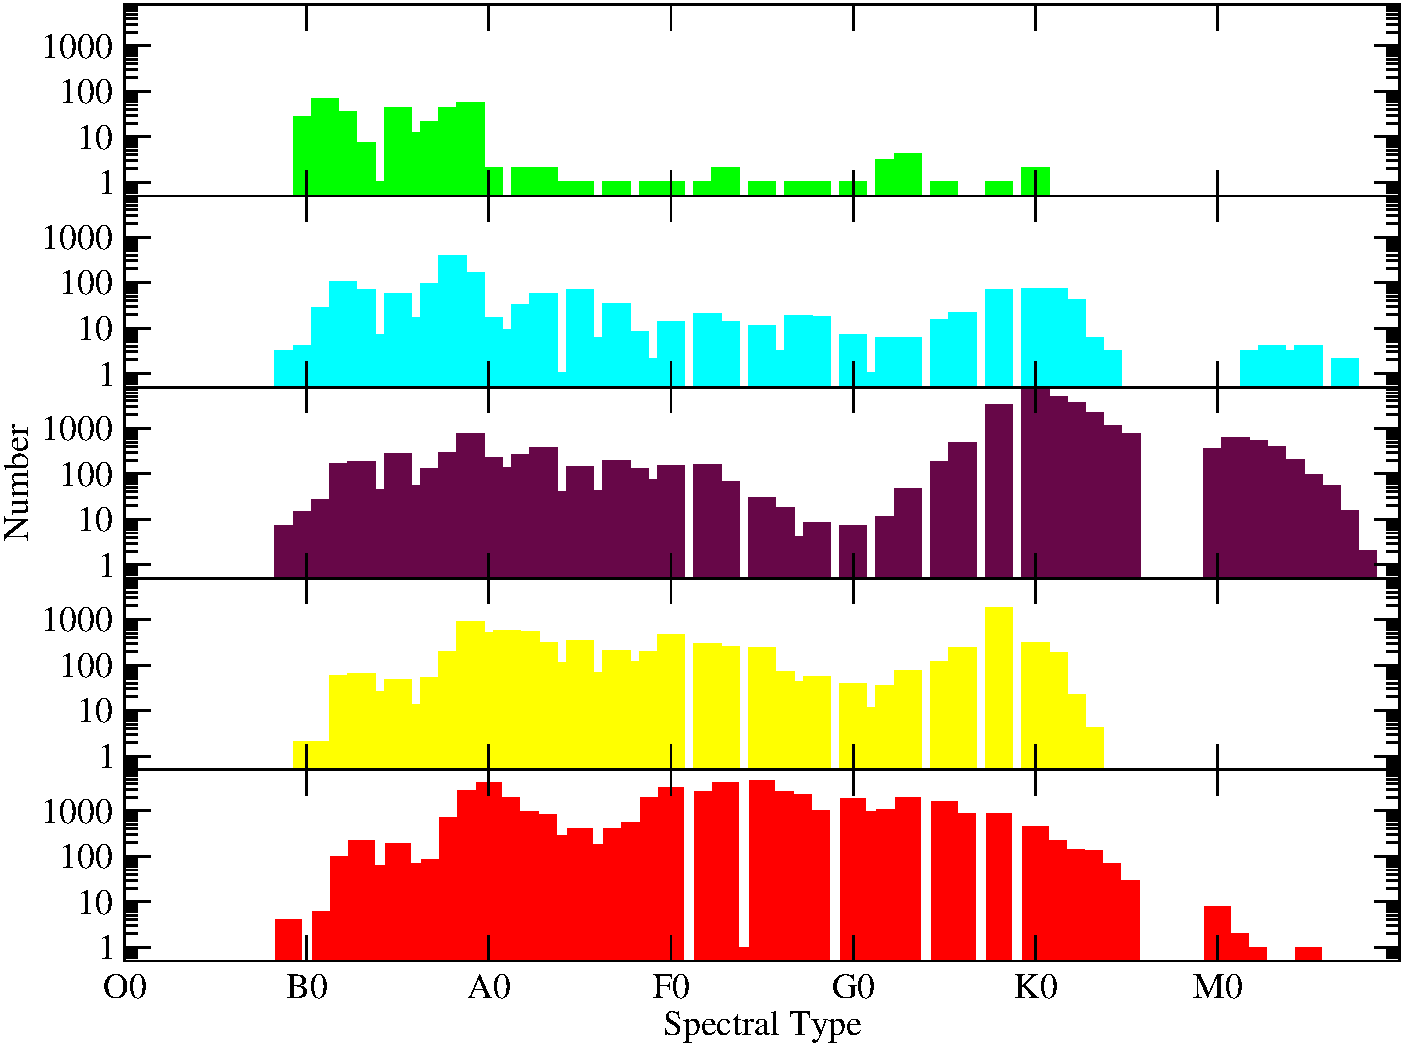
\includegraphics[width=1.0\textwidth]{Figures/populations/hist-spt-count.pdf}
\caption{The distribution of the Michigan Spectral Catalogs as a function of spectral type on the horizontal axis, after the removal of peculiar and/or mixed spectral types.  The different colors correspond to the different luminosity classes.  From bottom to top: V (red), IV (yellow), III (purple), II (cyan) and I (green).  The gaps in the histograms at particular spectral types (e.g. F1, K7-K9) indicate that this spectral type was not used for typing in the Michigan Spectral Catalogs.} \label{fig:spt_michigan_hist}
\end{figure}

\begin{figure}
    \centering
    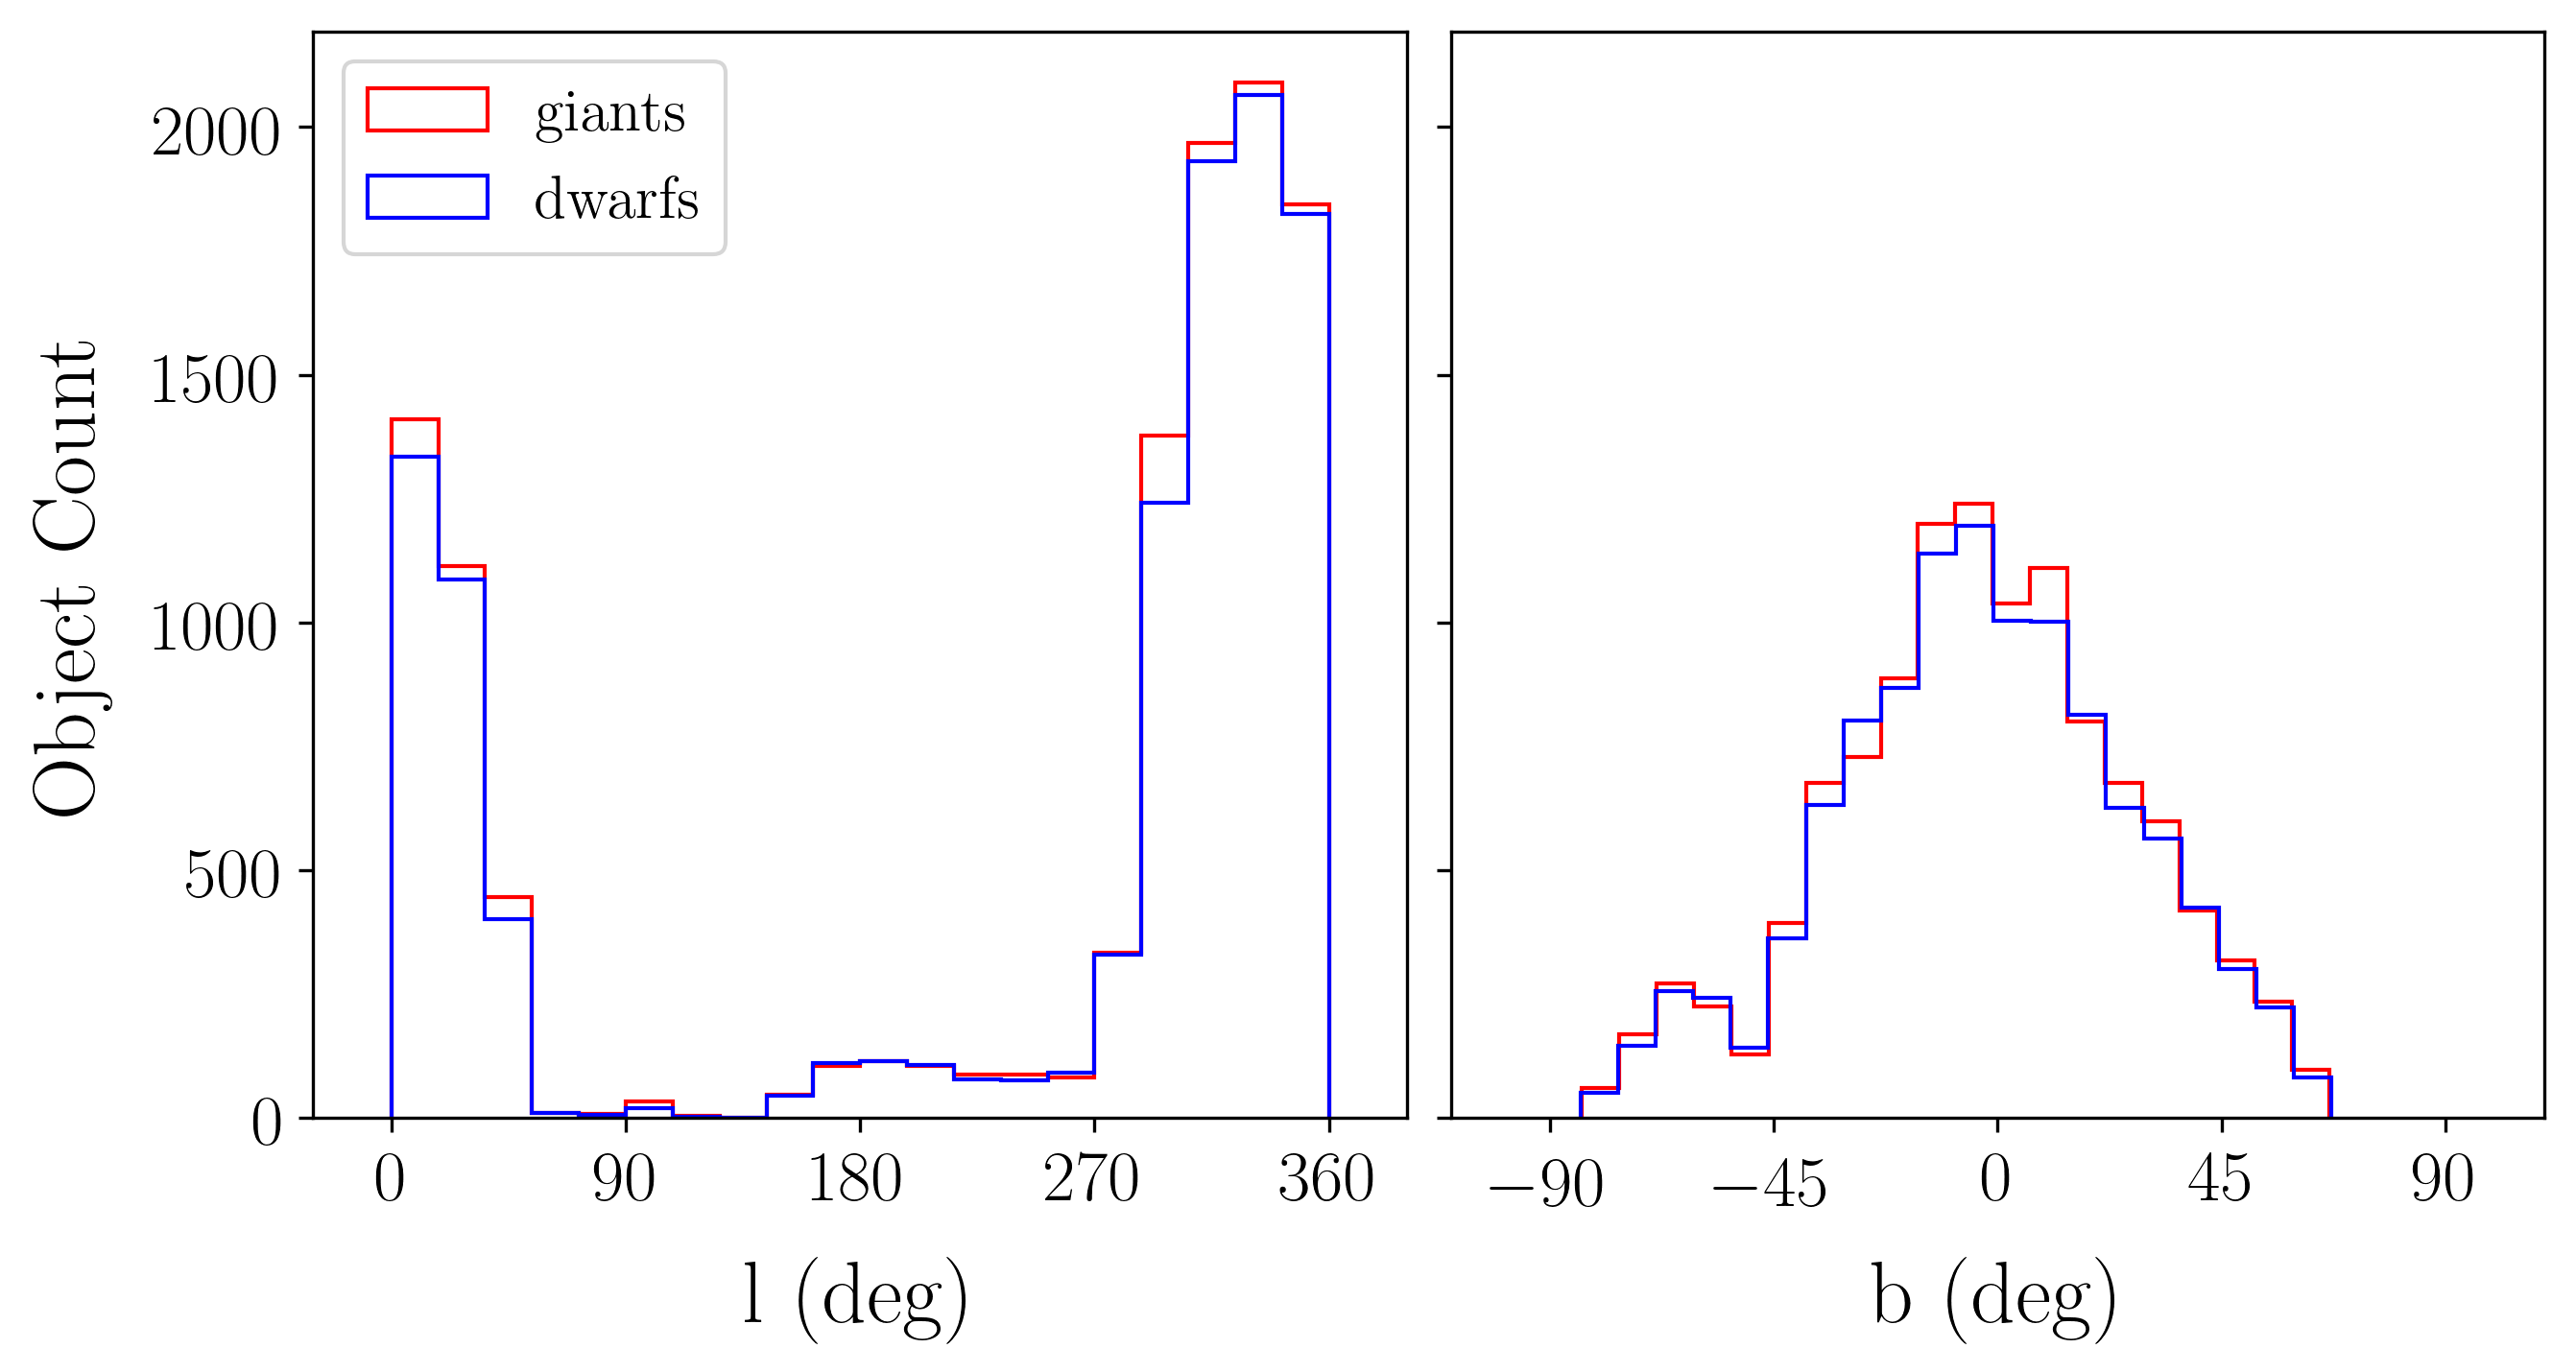
\includegraphics[width=1.0\textwidth]{Figures/populations/hist-b-vs-count.png}
    \caption{A histogram of spectra counts across all galactic latitudes ($b$) from the Michigan Spectral Atlas, which was filtered as described according to Chapter \ref{sec:cross-matching}. There is no large discrepancy of either luminosity groups.}
    \label{fig:b-vs-count}
\end{figure}

\begin{figure*}[t]
\centering
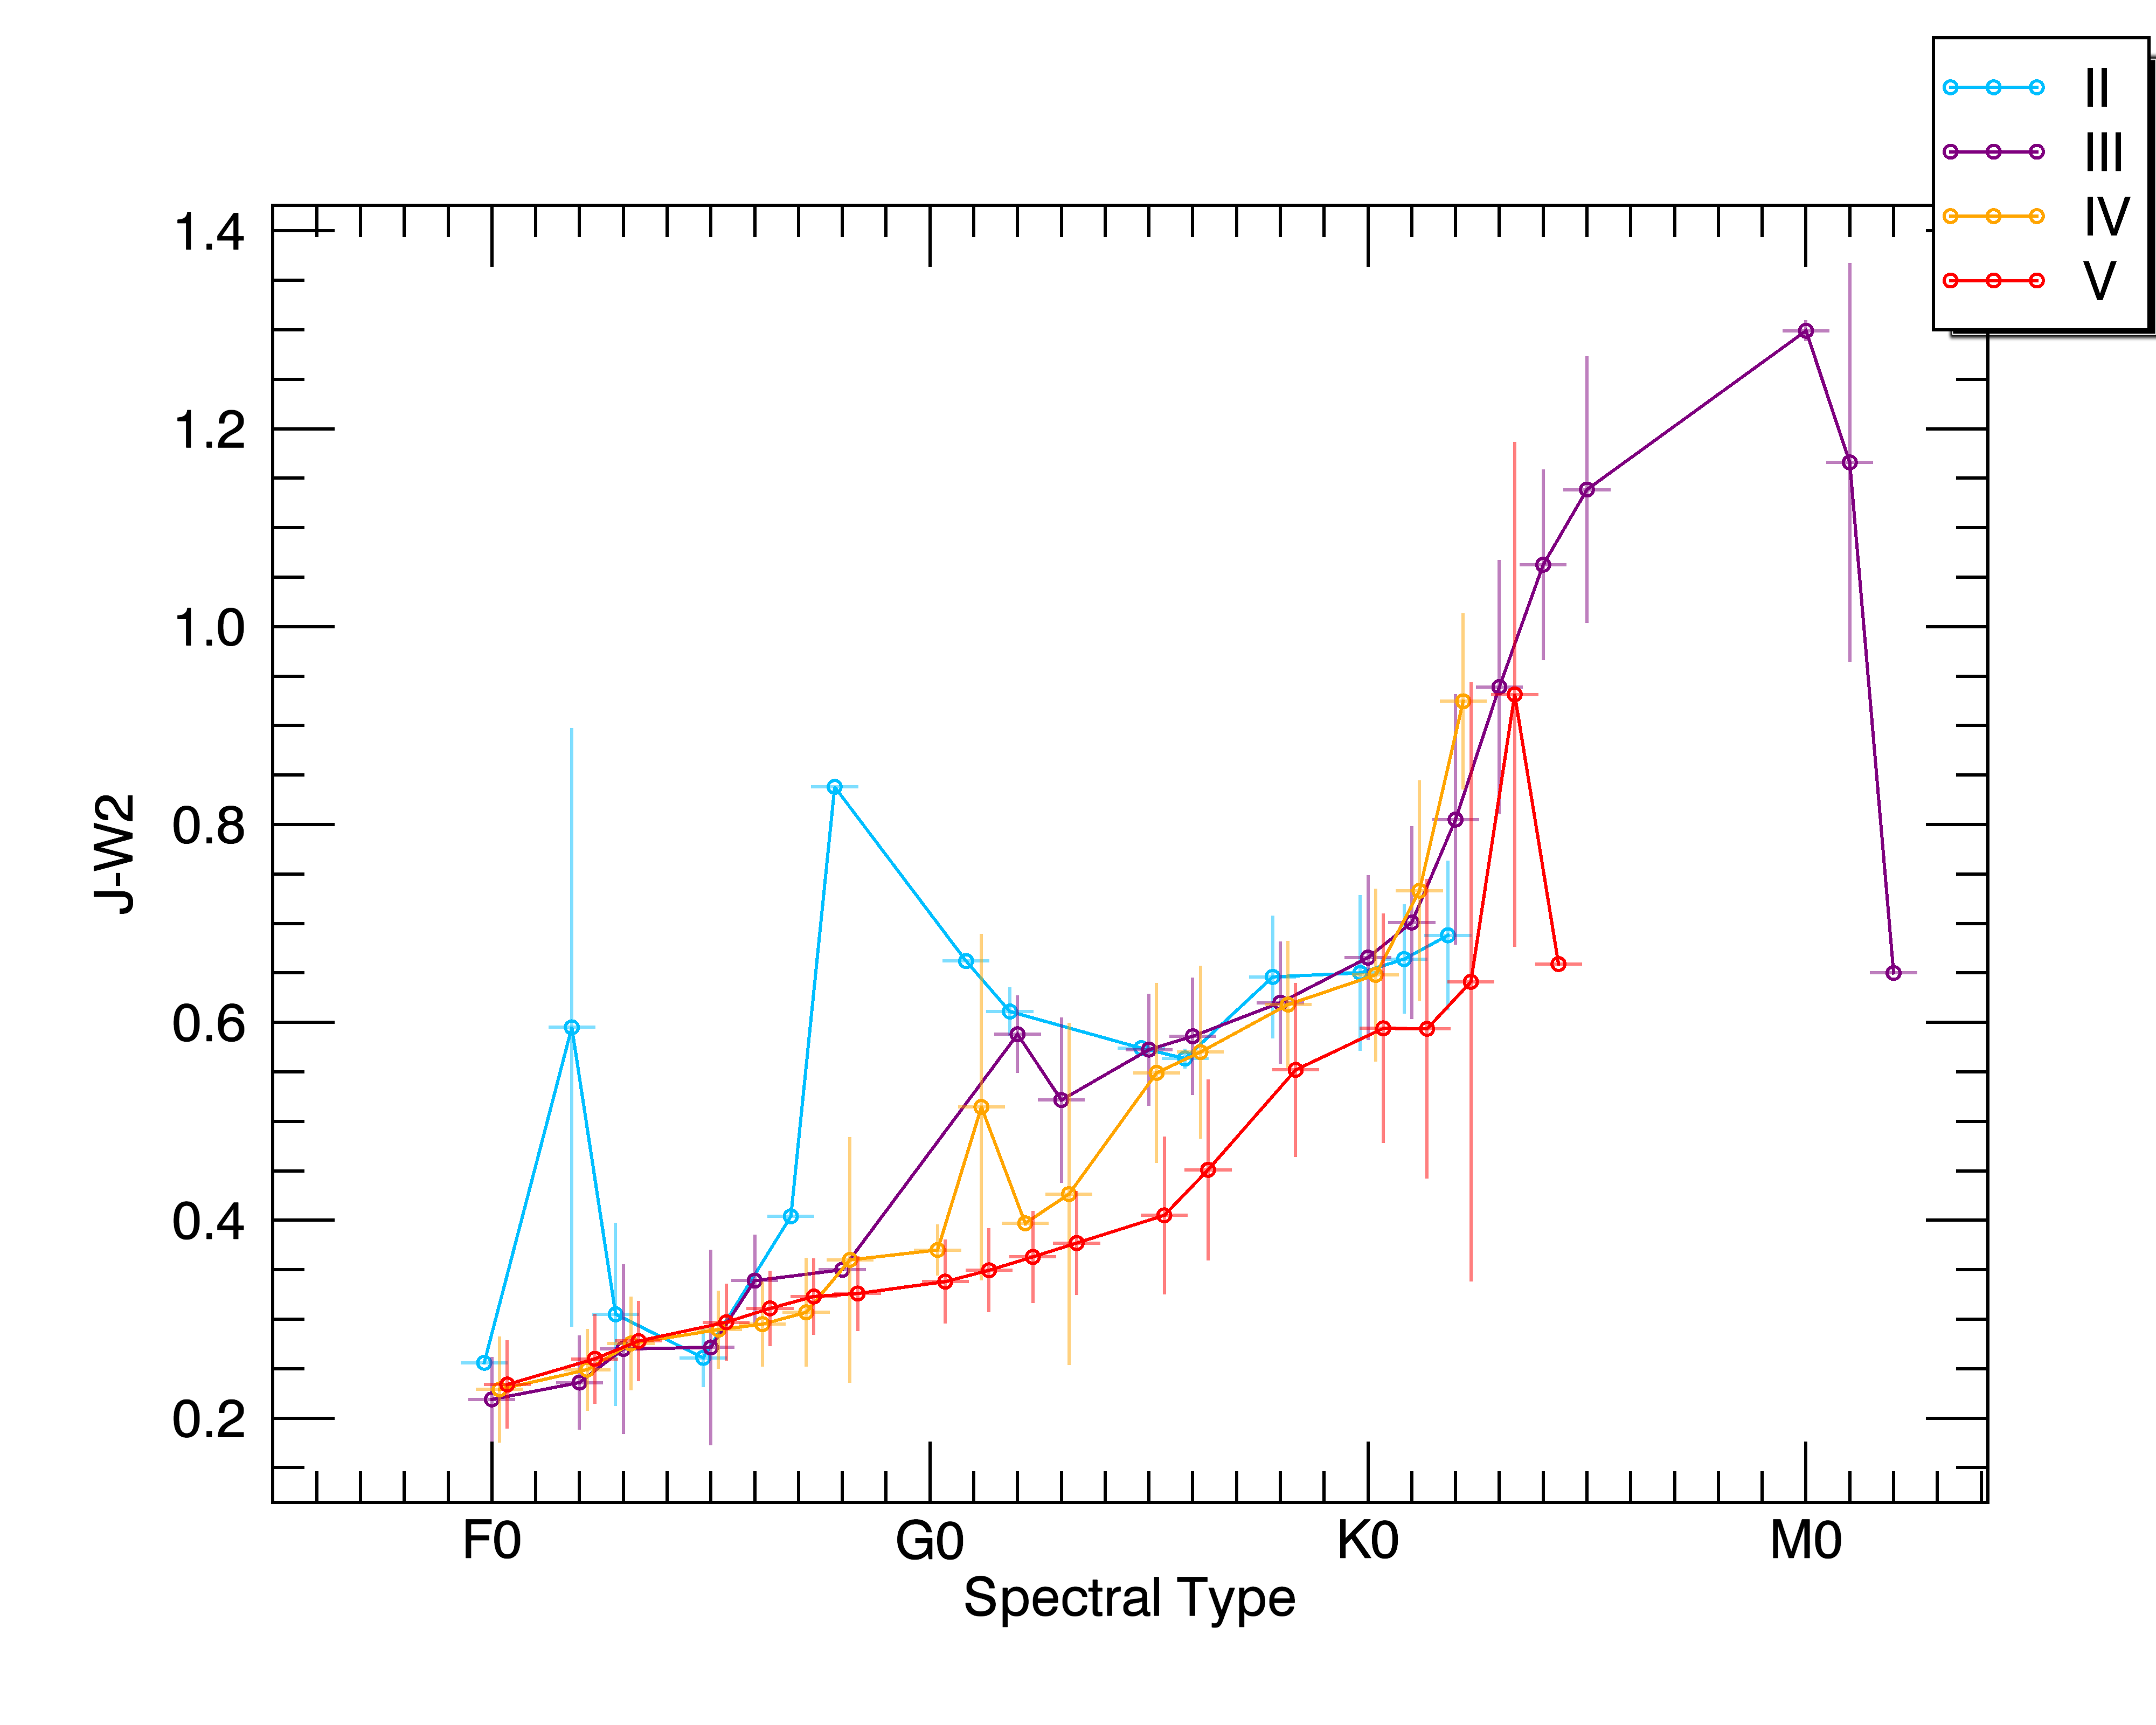
\includegraphics[width=1.0\textwidth,clip=true]{Figures/subtype_bar/SPT_J-W2.png}
\caption{The color of stars in the Michigan Spectral Catalogs as a function of spectral type on the horizontal axis, and \jwtwo on the vertical axis, after the removal of peculiar and/or mixed spectral types (see Chapter \ref{sec:cross-matching}). The different colors correspond to the different luminosity classes -- V (red), IV (yellow), III (purple), II (cyan) and I (green).  The vertical error bars generally correspond to the robust standard deviation of the \jwtwo color of stars within a given spectral type and luminosity class, unless there are only three or fewer stars, in which the error bars represent a standard deviation or range (see Chapter \ref{subsec:median_stats}, and Tables \ref{table:color_medians}). In order to see this type of figure for any other WISE and 2MASS colors as mentioned in Chapter \ref{subsec:median_stats}, see Appendix \ref{Appendix:2}.} \label{fig:median_stick_bar_jw2}
\end{figure*}

\begin{figure*}[t]
\centering
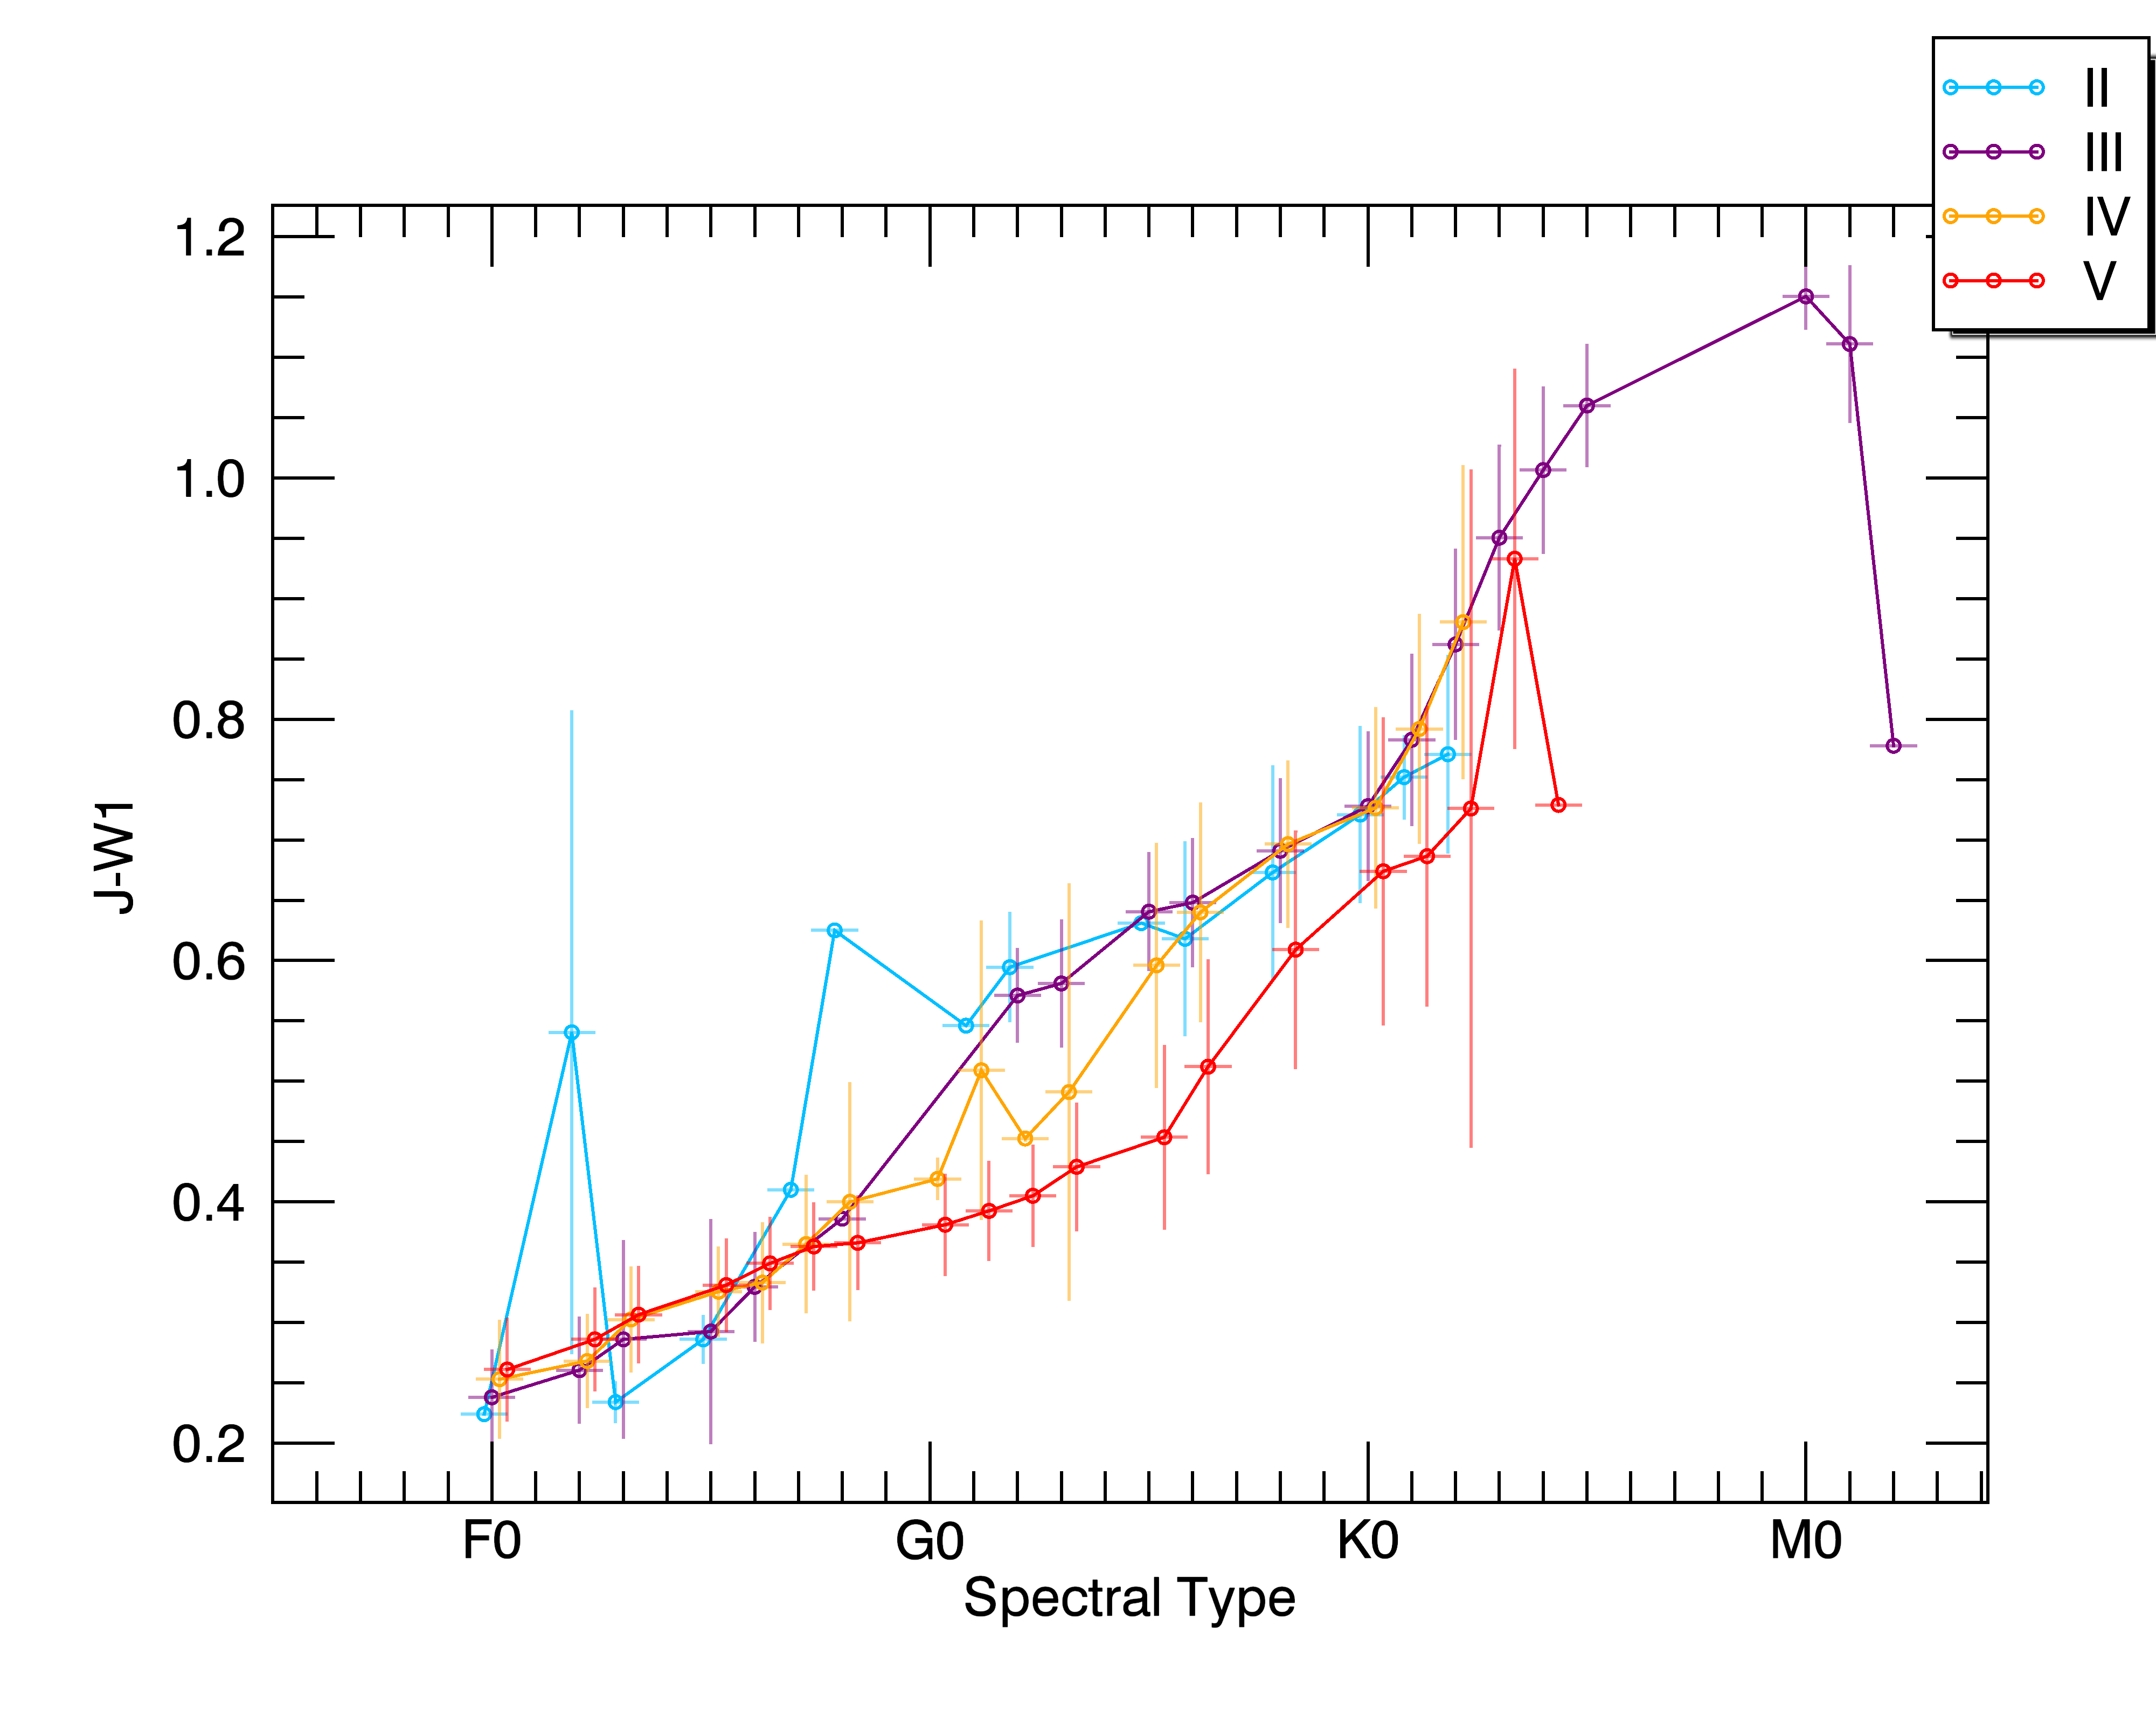
\includegraphics[width=1.0\textwidth,clip=true]{Figures/subtype_bar/SPT_J-W1.png}
\caption{Same as Figure \ref{fig:median_stick_bar_jw2}, but for $J-W{1}$.} \label{fig:median_stick_bar_jw1}
\end{figure*}

\chapter{Significance of \jwone and \jwtwo for GK stars}\label{chap:3}
% TEXT ==========================================

We identify by eye from the median color plots (e.g., Figures \ref{fig:median_stick_bar_jw1} and \ref{fig:median_stick_bar_jw1}) for all WISE/2MASS colors that \jwone and \jwtwo present a significant separation in color between dwarfs and (sub-)giants for all G and early K spectral types. This trend in \jwone and \jwtwo with luminosity class for G and early K dwarfs may extend to later spectral types (M stars), but the limited number of M dwarfs in the Michigan Spectral Atlases precludes a robust determination.

The separation is approximately one robust standard deviation of the colors for a given spectral type and luminosity class. For example, the color distribution of G5V stars is $J-W2=0.405\pm0.078$, for G5III stars is $J-W2=0.573\pm0.055$, a difference of $0.168\pm0.095$ of more than one standard deviation. While there is significant overlap in the colors of stars of different luminosity classes, this still permits a probabilistic assignment of luminosity class which we explore further in Chapter \ref{chap:4}.

The robust standard deviation of the colors of a given spectral type and luminosity class in the spectral type range of interest (G0-K5) is consistent with typical WISE and 2MASS magnitude measurement uncertainties ($\sim$0.05--0.15 mag). Thus, this implies the overlap in the dwarf-giant color distributions may be due to measurement uncertainties rather than a physical origin.  More precise color measurements may increase the statistical significance of this separation between dwarfs and (sub-)giants in color. How to utilize color separation, also seen in the color probability functions created in Chapter \ref{subsec:tdist_stats}, is discussed and visualized in specific detail in Chapter \ref{sec:color_prob_func}. 

In the next sections, we turn to highlighting sample applications of utilizing this primary result for use in distinguishing dwarfs from giants.

\section{Possible origins of dwarf-giant color separation}

We have considered two possibilities for this observable difference in the infrared colors of dwarf stars compared to giant stars. We have considered that the source of the color difference is due to (1) observational bias from reddening due to galactic extinction, or is (2) astrophysical in origin, which would help underline the intrinsic physical difference of dwarfs from giant stars. We stipulate that while there is a possibility both (1) and (2) could be contributing to the color difference we do see among different luminosity classes, it is more likely that (2) is the more dominant effect, which has interesting astrophysical implications in characterizing dwarfs from giants stars. 

We infer that (2) is more likely than (1) because we have examined the medians magnitudes of colors, for which we had greatest separation (\jwone and \jwtwo), across the galactic latitude coordinate $b$. We consider $b$ since it can assess whether galactic extinction may have contributed more reddened colors that could have explained this color separation (Figure \ref{fig:color-vs-b}). We estimate that any reddening effect due to extinction should be strongest at the sky area that covers the galactic plane where gas clouds are concentrated, at approximately $|b|<15$. Median color does not typically spike in the galactic plane for both \jwone and \jwtwo while in the same luminosity group (Figure \ref{fig:color-vs-b}), which suggests that the color separation between dwarfs and giants is not due to extinction, but from astrophysical cause, such as gravity-sensitive lines in J-band.

% FIGURES ==========================================

\begin{figure}
    \centering
    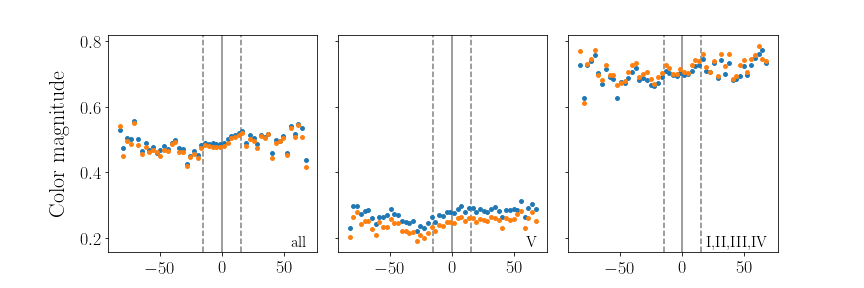
\includegraphics[width=1.0\textwidth,clip=true]{Figures/populations/plot-b-vs-color.png}
    \caption{This figure displays the median values of color magnitude \jwone and \jwtwo across galactic latitude for different luminosity classes. Colors magnitude and luminosity class information originate from a cross-matched table of WISE/2MASS with the Michigan Spectral Atlas, and no extinction correction has been applied. There is no considerable reddening of color for latitudes that contain the galactic plane ($|b|<15$), which suggests the color separation is not extinction dependent.}
    \label{fig:color-vs-b}
\end{figure}

\chapter{Using color separation as a stellar characterization tool}\label{chap:color_as_tool}
% TEXT ==========================================

\section{Color probability density functions}

\section{Applicability to modern surveys}
Therefore J is just damn special, and it would be a subject of future work as to why J band spectral features are gravity sensitive for GKM dwarfs (J-K for M dwarfs) and J-W1/2 for GK dwarfs.

We also note the importance the J-band is in differentiating between dwarfs from giants given its previously proved sensitivity for differentiating M dwarfs from GK dwarfs for J-K (REF). The combination of this study with J-W1/2 in being sensitive for GK dwarfs, and J-K being sensitive for GKM stars suggests the presence of surface gravity sensitive lines in the J-band. Thus, there we suggest it is viable to search for gravity sensitive lines along these the J-band wavelength range.

% FIGURES ==========================================

\begin{figure}
    \centering
    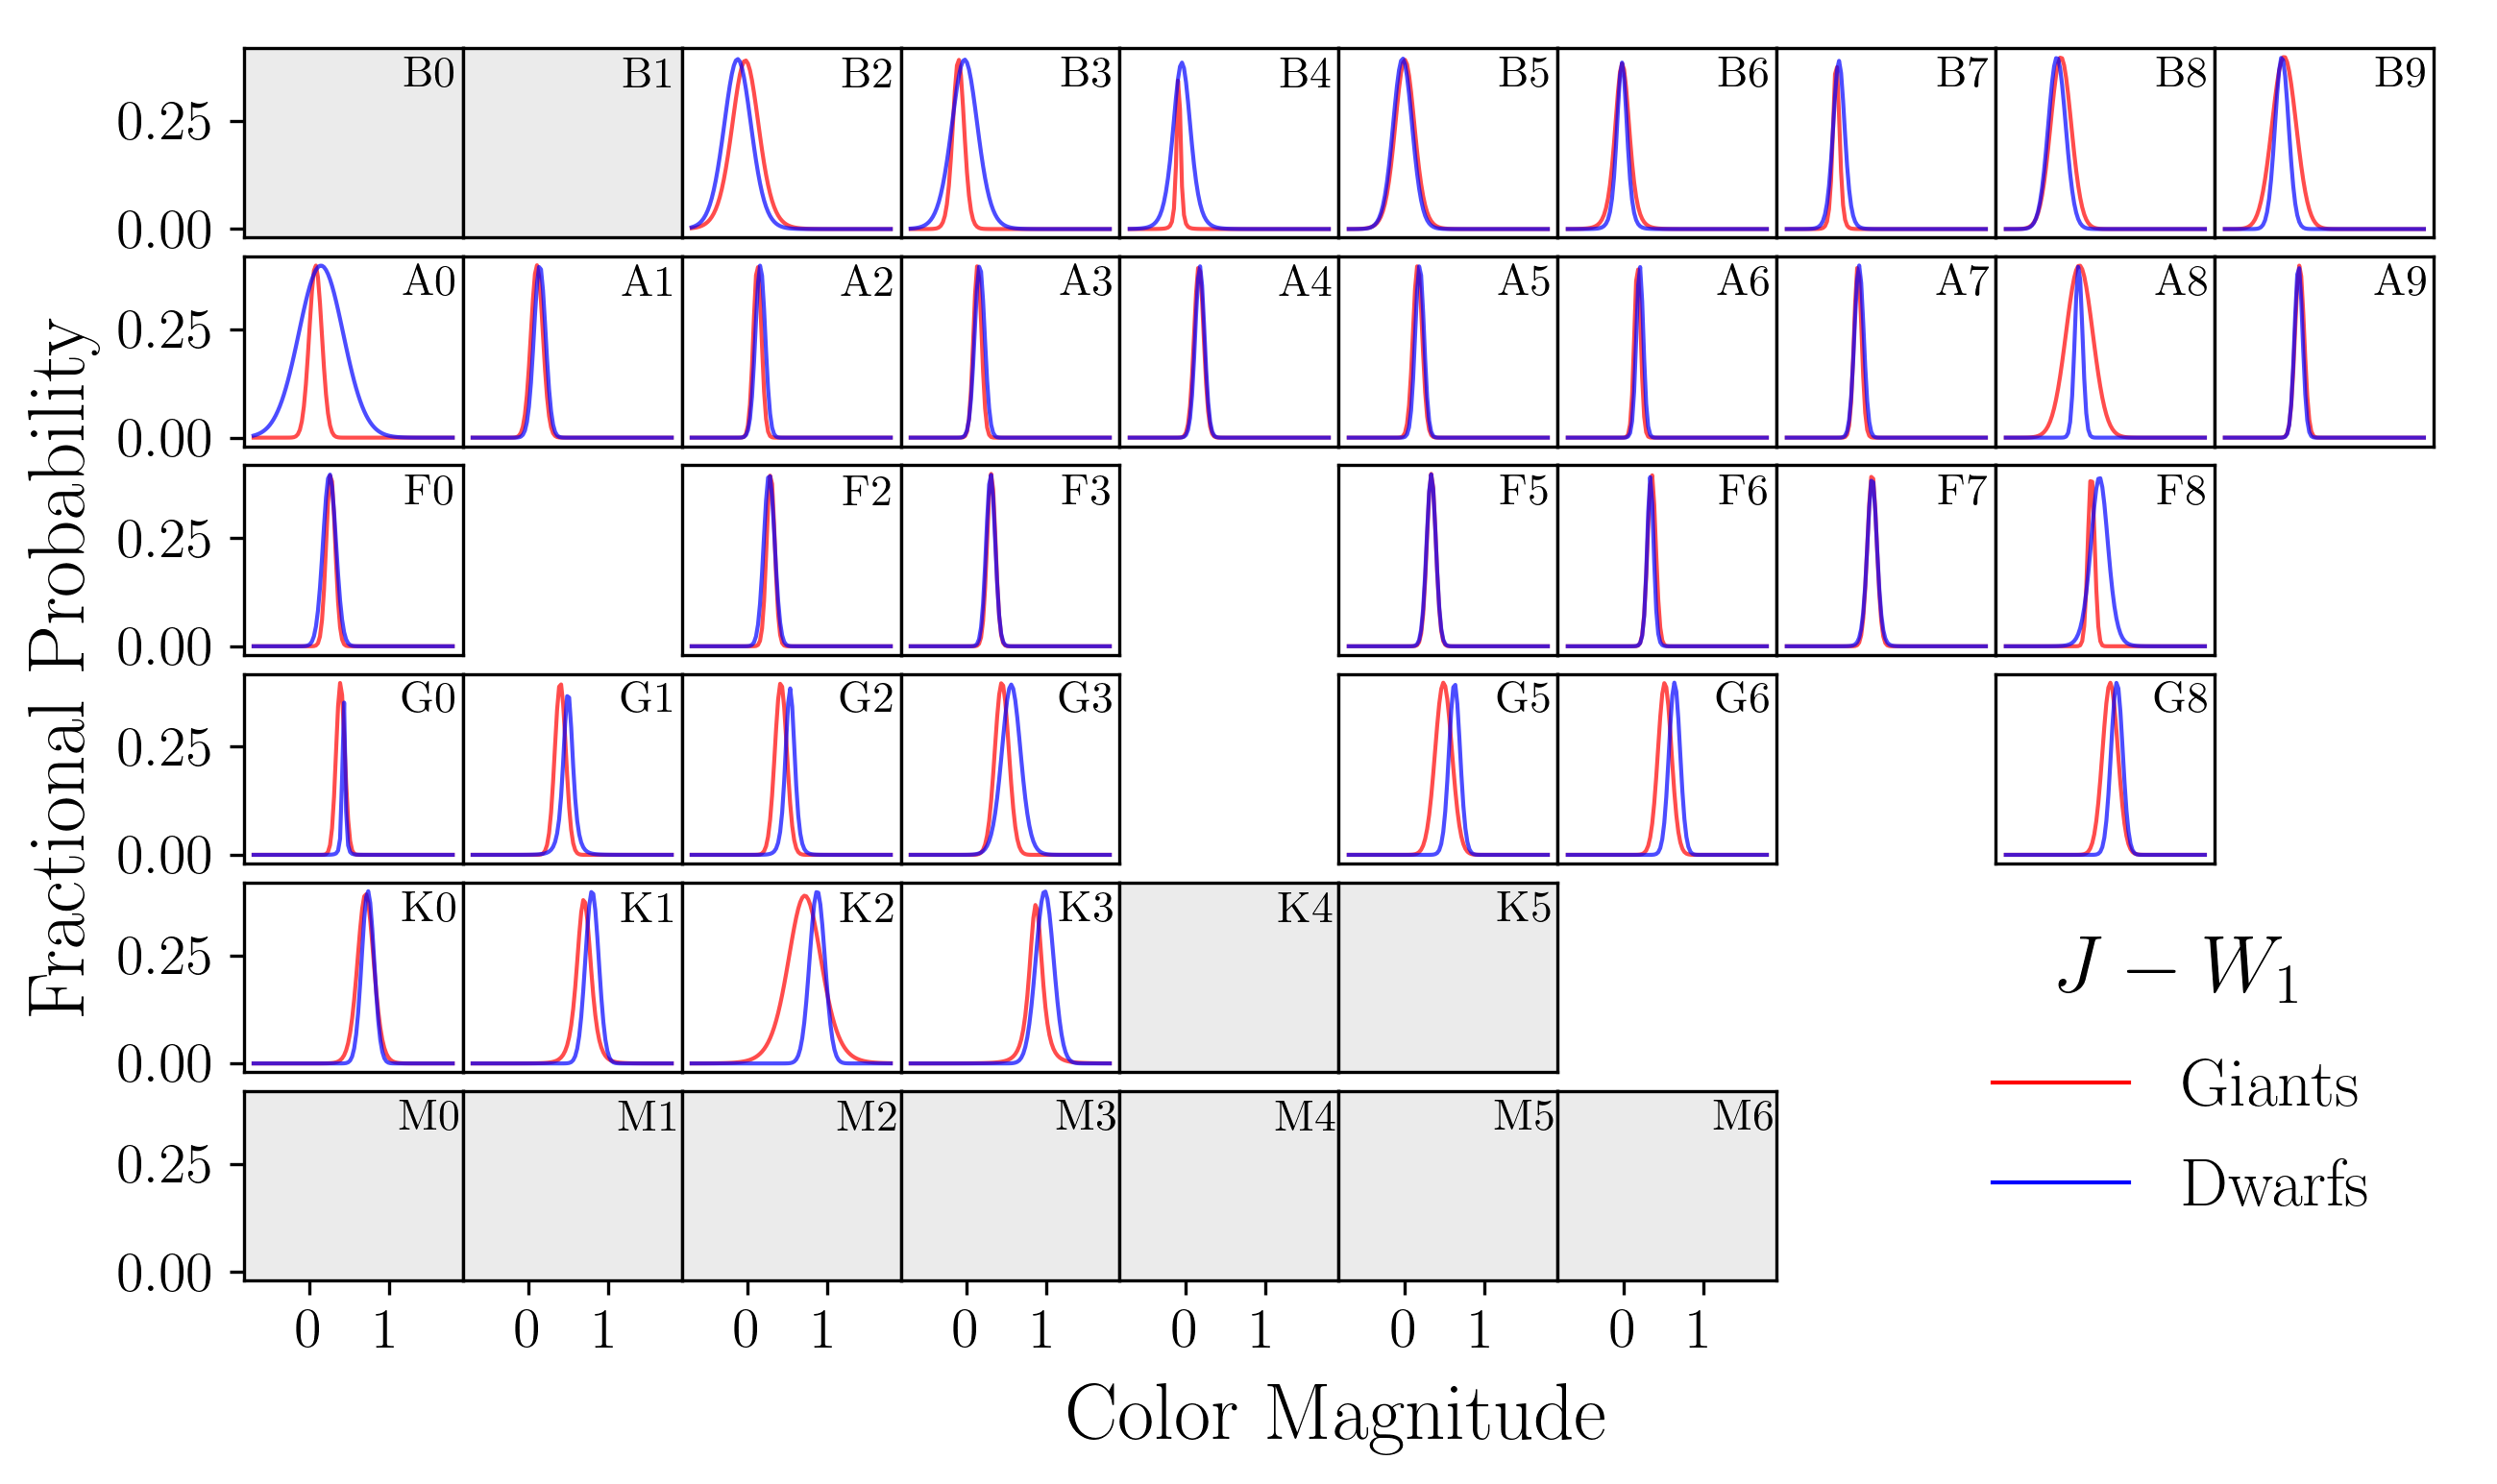
\includegraphics[width=1.0\textwidth,clip=true]{Figures/periodic/periodic-t-pdf_J_W1.png}
    \caption{Caption}
    \label{fig:periodic-pdf-jw1}
\end{figure}

\begin{figure}
    \centering
    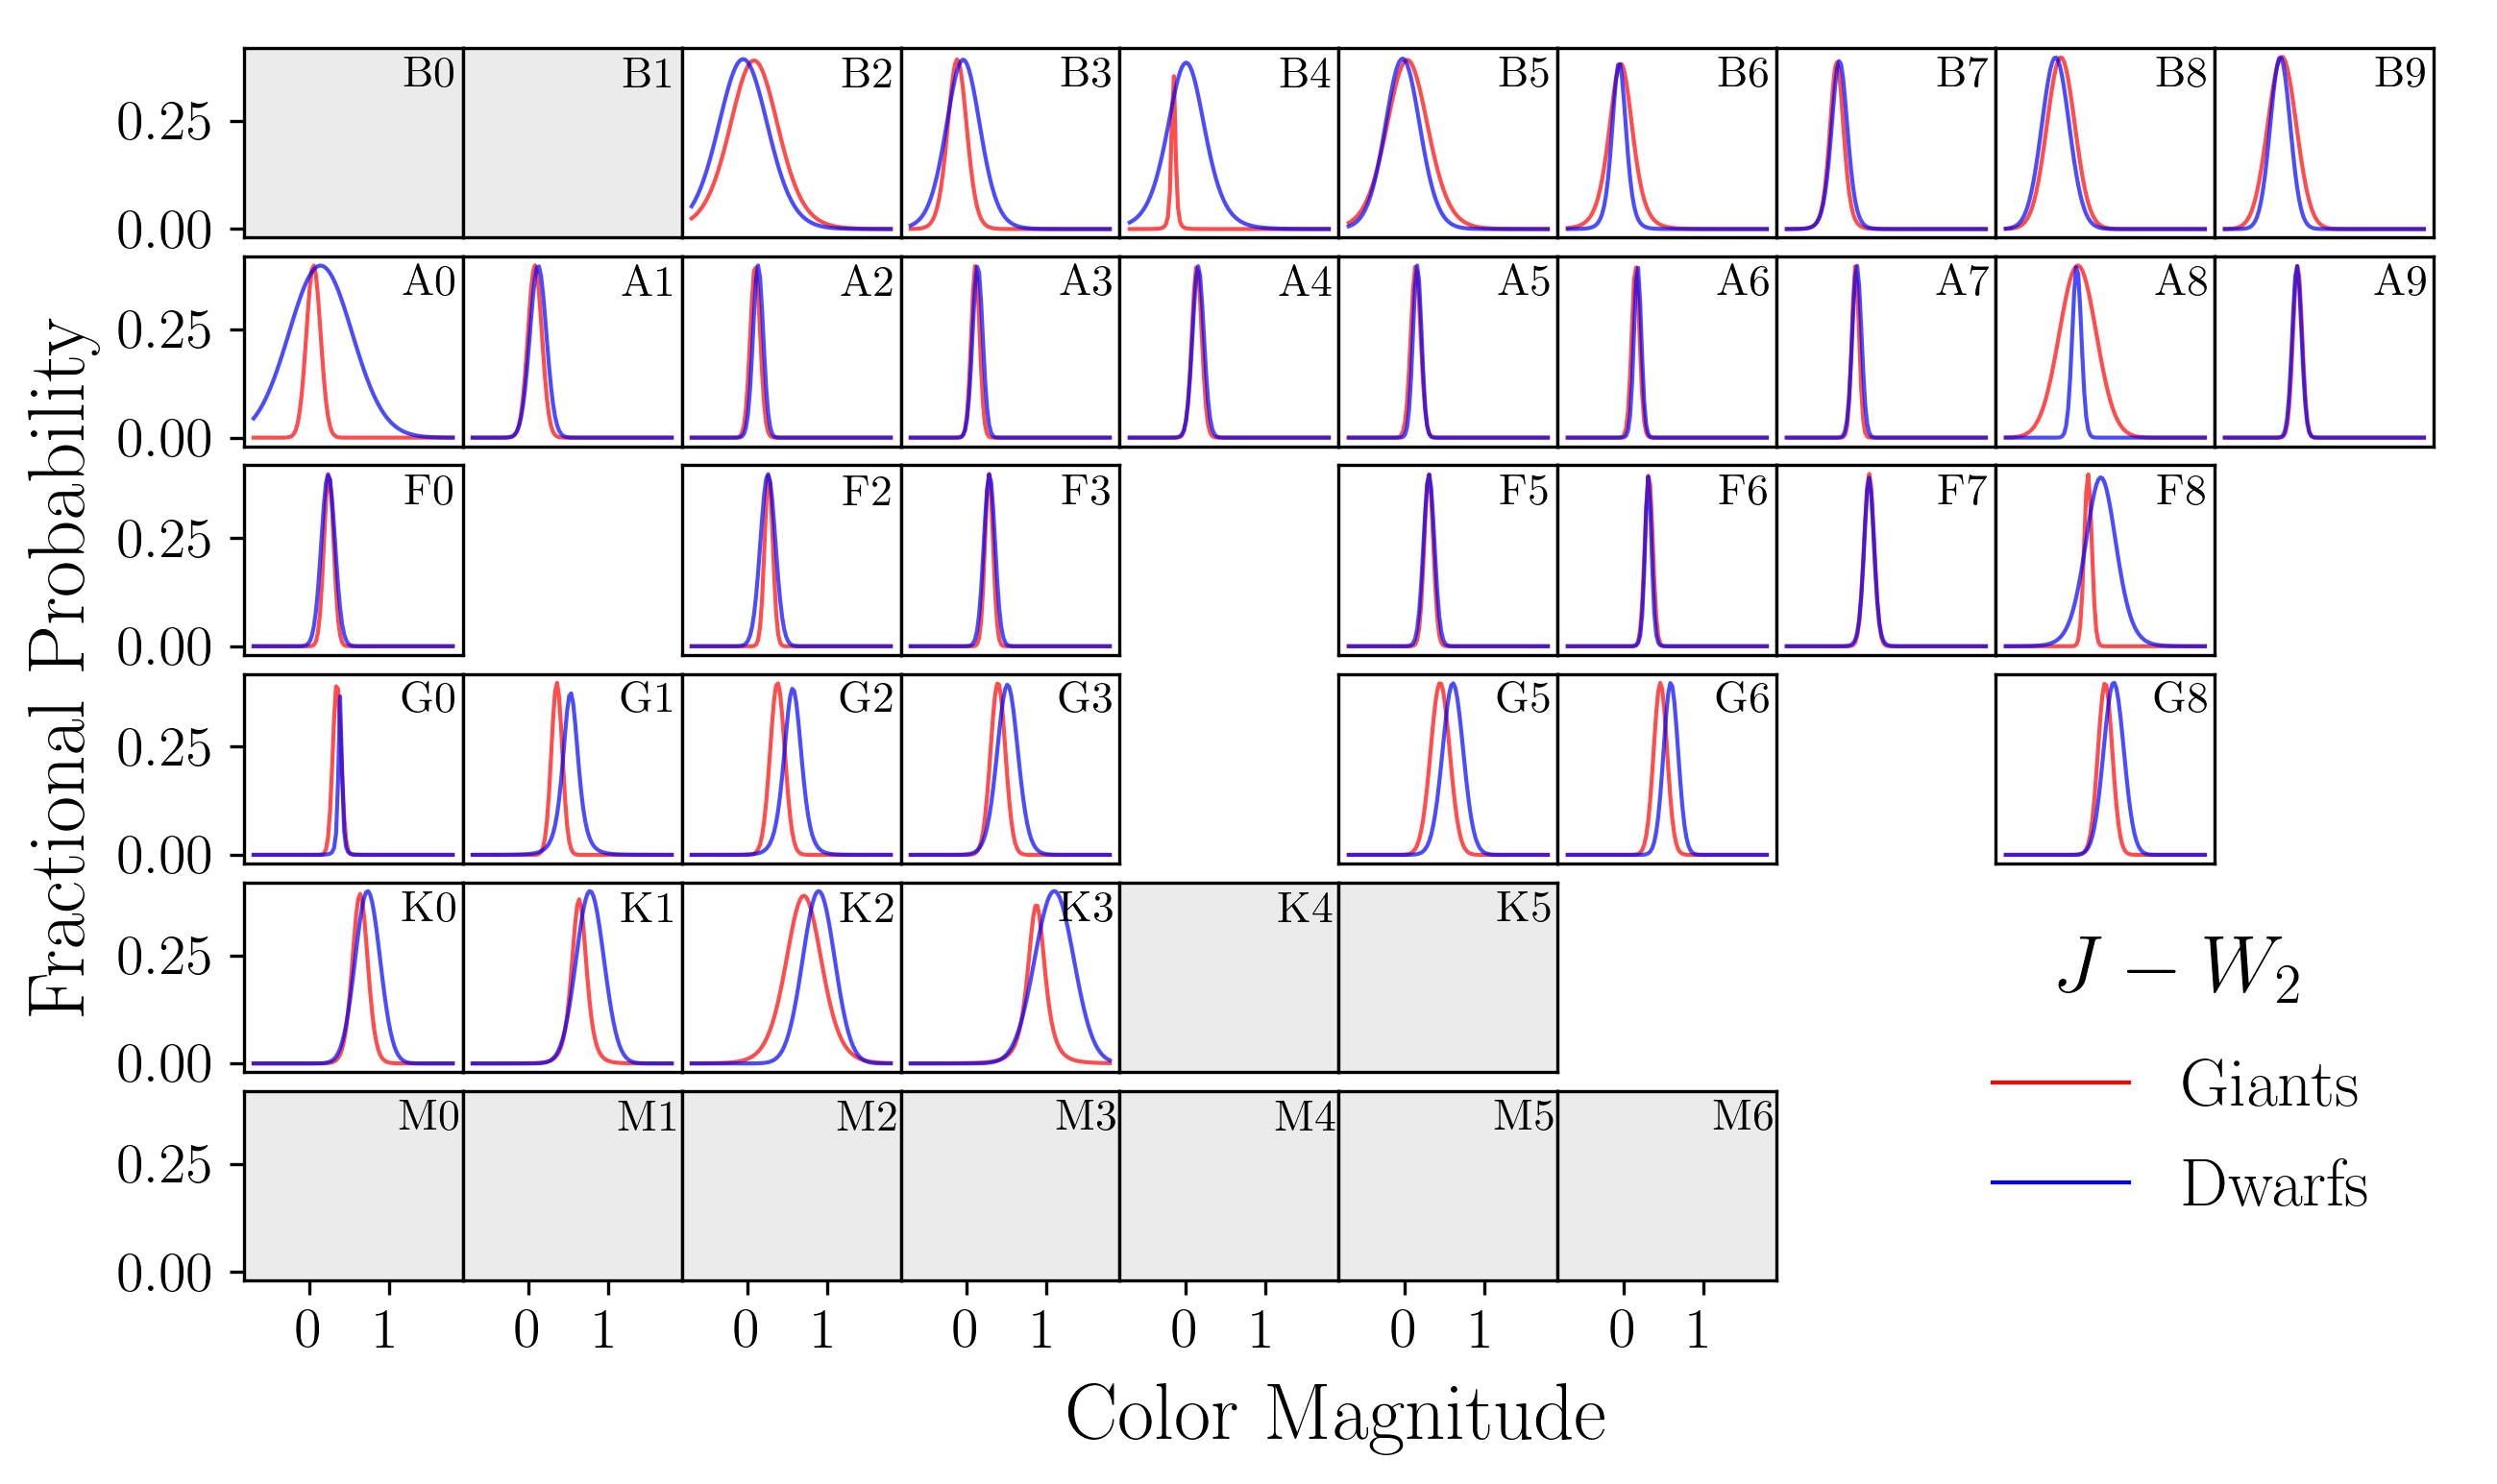
\includegraphics[width=1.0\textwidth,clip=true]{Figures/periodic/periodic-t-pdf_J_W2.png}
    \caption{Same as Figure \ref{fig:periodic-pdf-jw1}, but for \jwtwo.}
    \label{fig:periodic-pdf-jw2}
\end{figure}

\begin{figure}
    \centering
    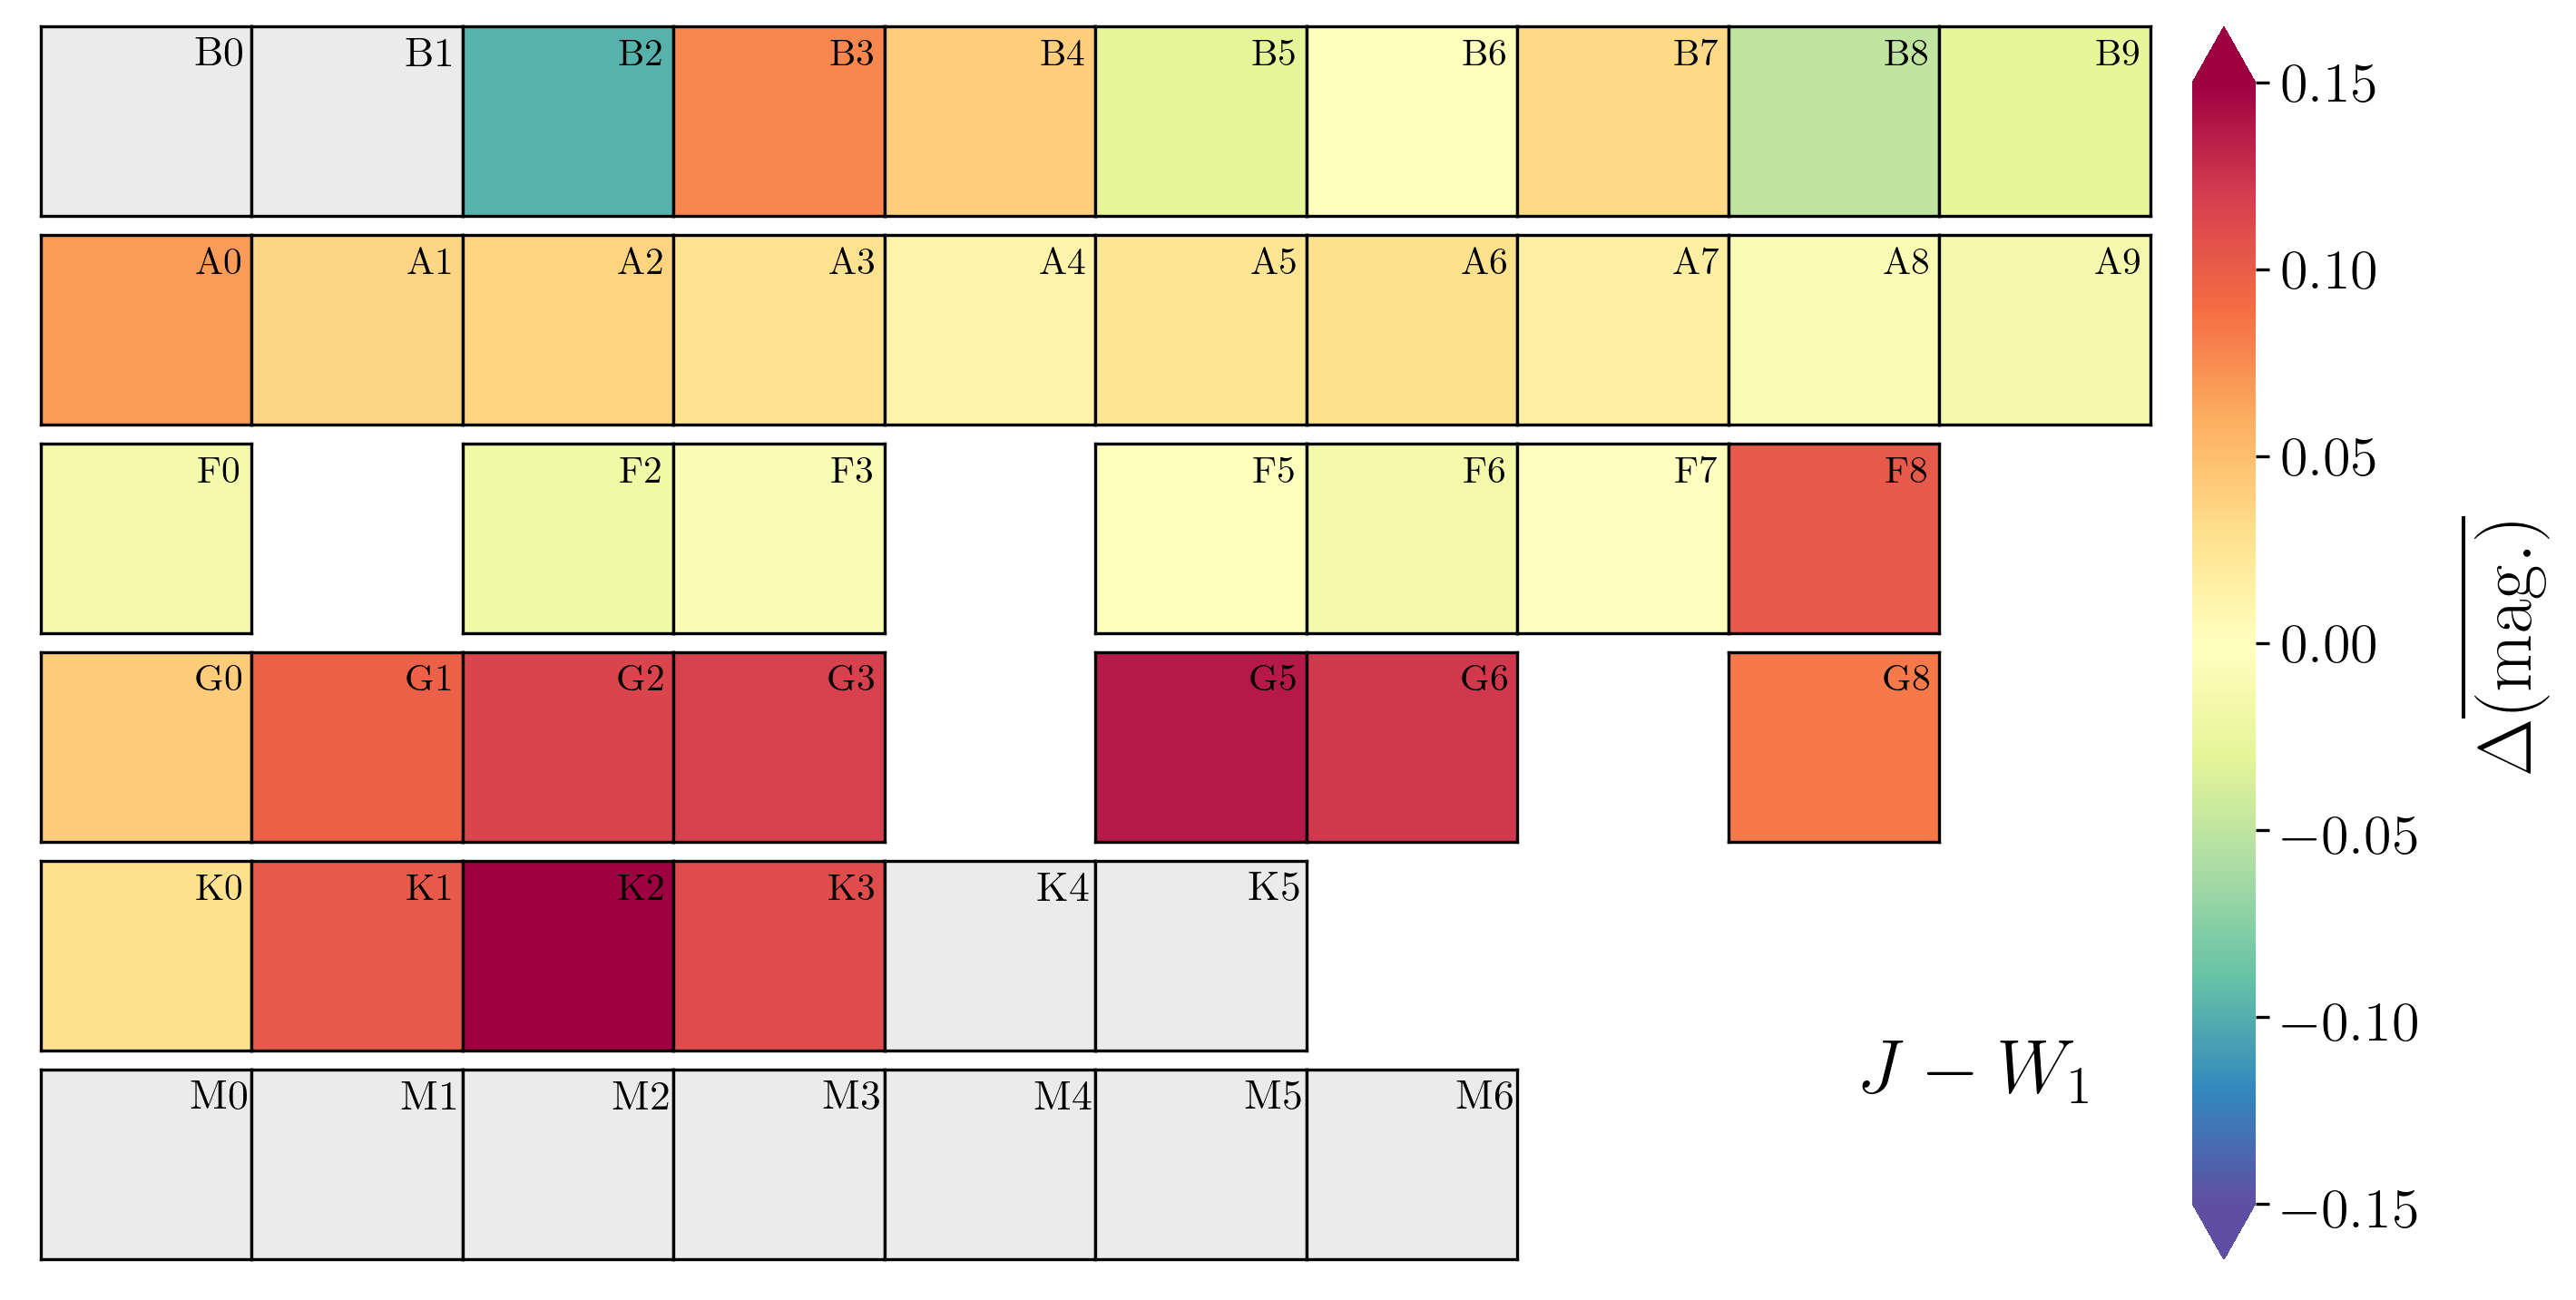
\includegraphics[width=1.0\textwidth,clip=true]{Figures/periodic/periodic-delta_J_W1.png}
    \caption{Caption}
    \label{fig:periodic-delta-jw1}
\end{figure}

\begin{figure}
    \centering
    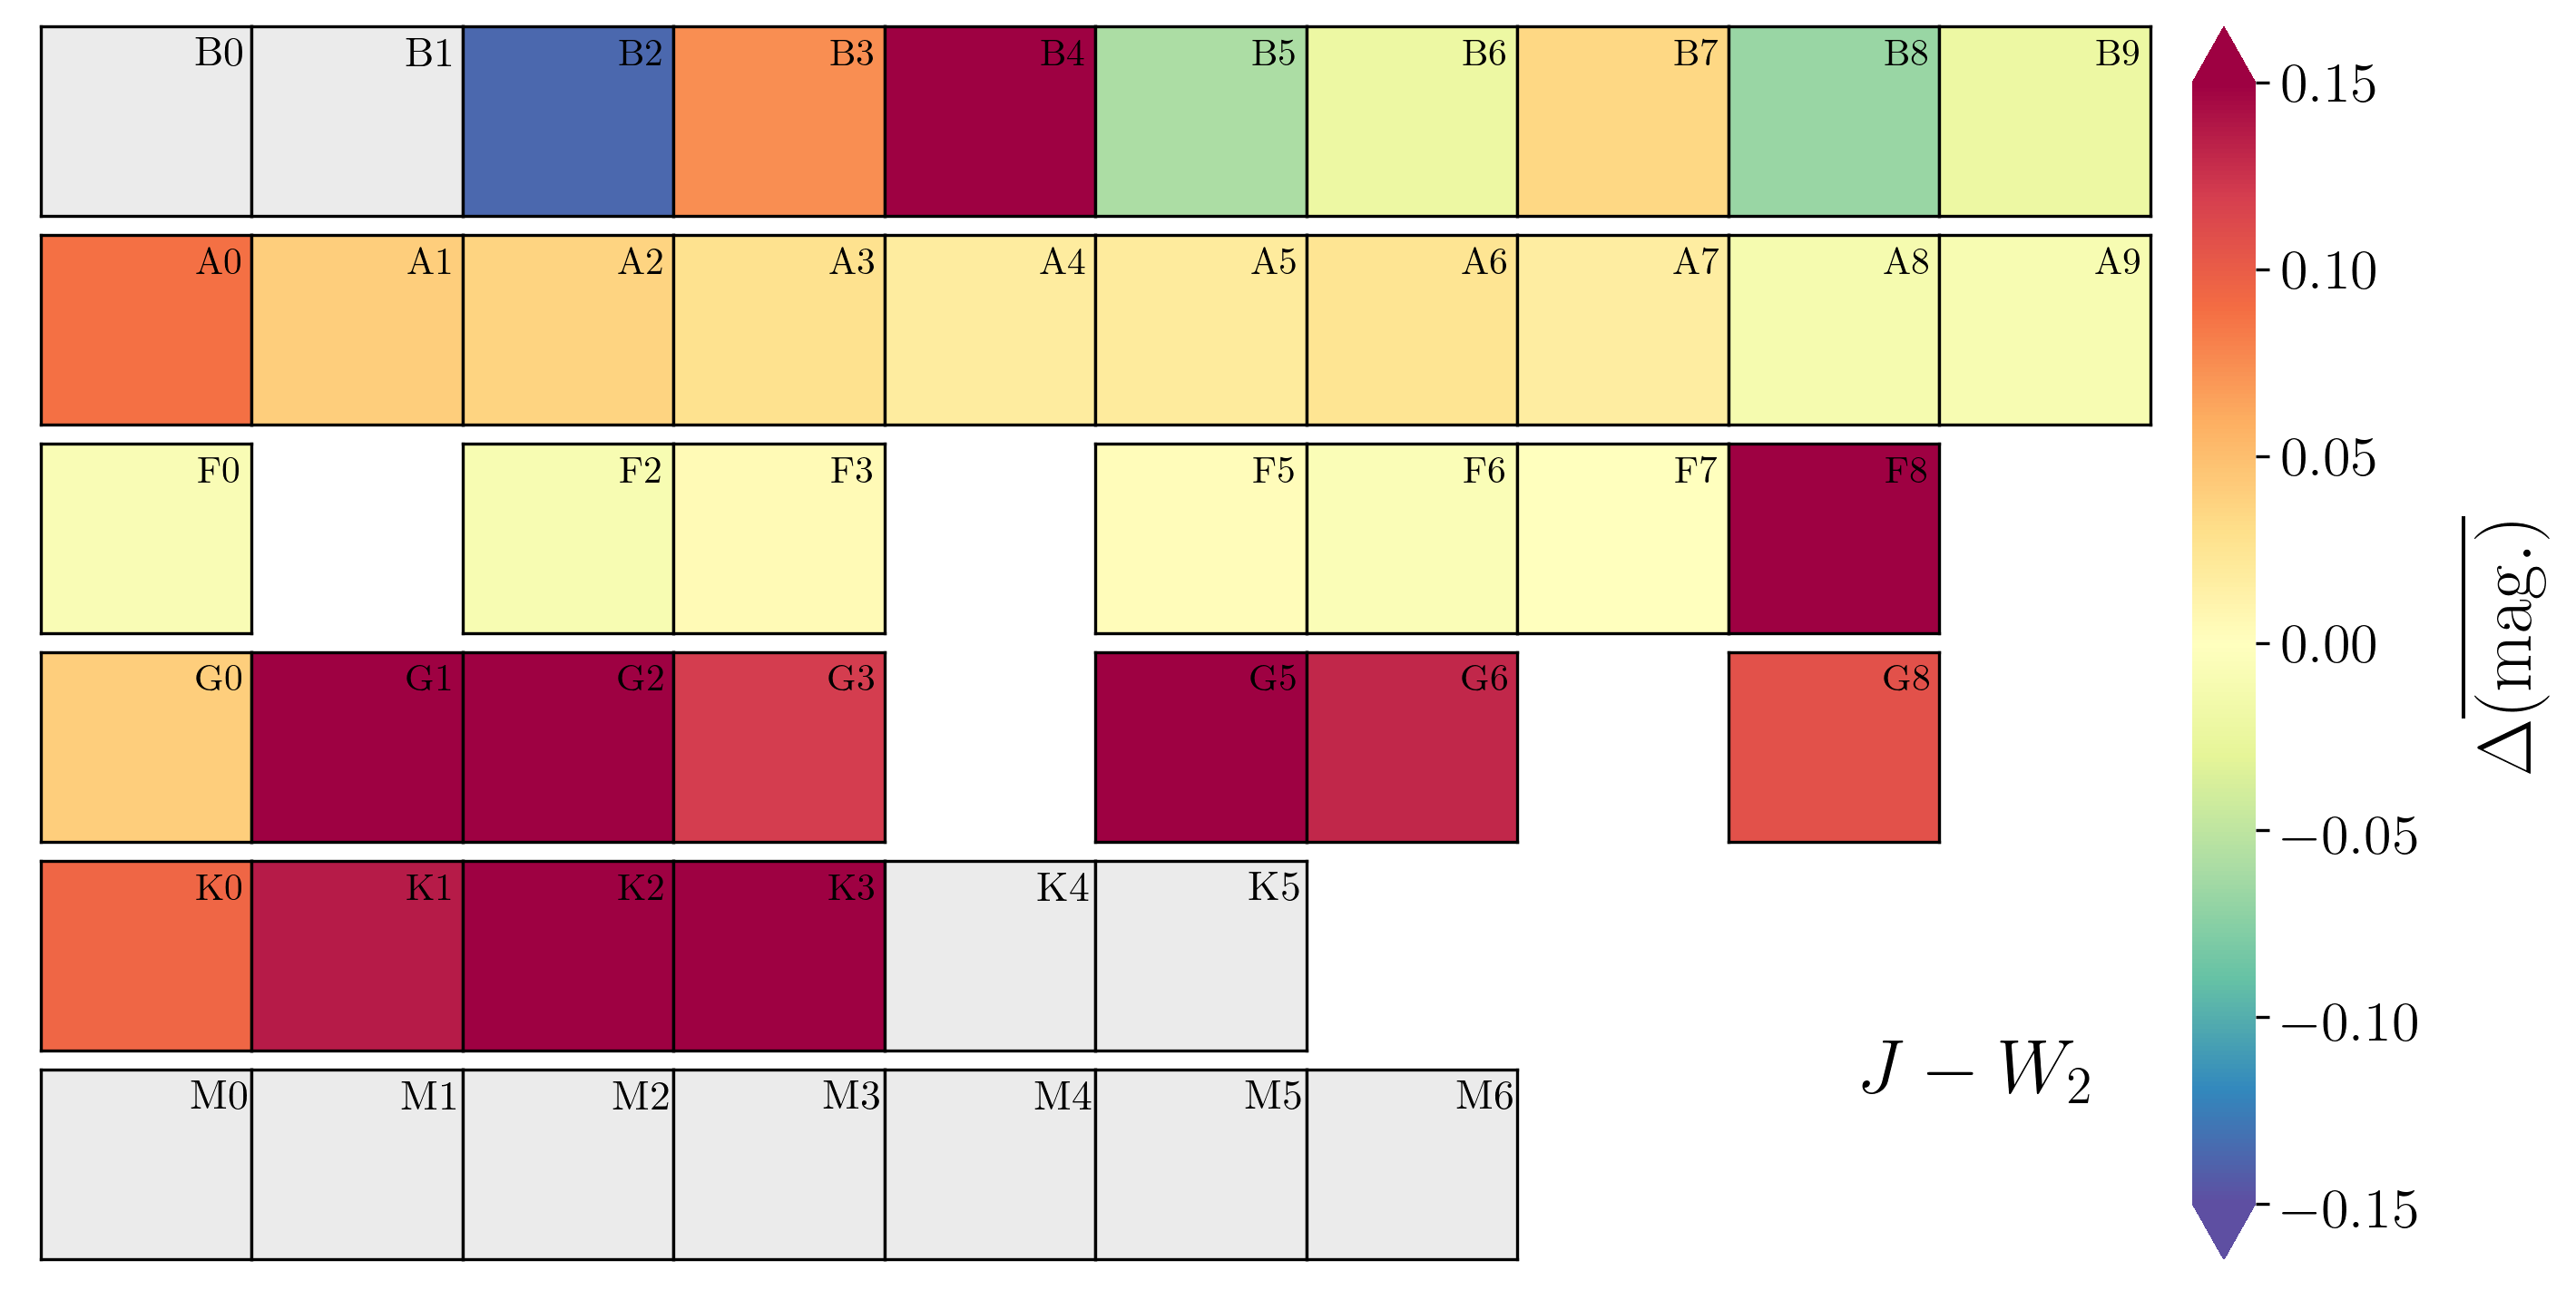
\includegraphics[width=1.0\textwidth,clip=true]{Figures/periodic/periodic-delta_J_W2.png}
    \caption{Same as Figure \ref{fig:periodic-delta-jw1}, but for \jwtwo.}
    \label{fig:periodic-delta-jw2}
\end{figure}


\chapter{Conclusion}\label{chap:conclusion}
% TEXT ==========================================

We have discovered a color separation between G-type and early K-type dwarf and giant stars that is statistically significant for \jwone and \jwtwo; giants stars (class $IV$ or below) are on average [filler stat] more red than their dwarf counterparts (class $V$) for the same spectral type. We can use this color separation to estimate luminosity class likelihood just from magnitude of the infrared color without needing extinction correction, as long as the star is estimated to be a G-type or early K-type. We can better constrain this luminosity class estimate by incorporating an artificial galactic population model with these infrared color magnitudes by a further [filler stat].

This luminosity class and color probability could also be incorporated into a Bayesian framework using other empirical measurements to improve the fidelity of surface gravity estimates for GKM stars in the absence of parallaxes, high resolution spectra, flicker analysis, or asteroseismology. 

The range and accuracy this luminosity class estimator tool is topped off due to the limited sample size of the Michigan Spectral Atlas Catalogs \citep{Houk1975,Houk1978,Houk1982,Houk1988,Houk1999} cross-matched to infrared catalogs 2MASS \citep{2MASS} and WISE \citep{WISE}. Few spectra are available in the atlas for M-types and very early types (OBA) because of the difficulty in obtaining decent quality observations for low luminosity targets and the rarity in stellar populations, respectively. Future improvements could include expanding the color-luminosity class estimation tool to these other spectral types. In order to do this, we would need obtain targets whose luminosity class and spectral type we can obtain with a high degree of certainty, and combined  infrared photometry, calibrate for the color difference in a similar fashion as we did for the G/K-types in this work. However, it is a possibility that a color difference between dwarfs and giants may not exist for these other spectral sub-types or for colors. In this case, one can explore different colors or even color-color combinations to see if a separation between dwarfs and giants do exist for various other parameter spaces, by adjusting spectral subtype, color, or luminosity class as experimental variables. Regardless, this poses potential to be a cheaper and efficient method of characterizing stars in bulk with only photometry and a spectral type estimate. It will be useful in the scope of future large-scale surveys and exoplanet characterization by constraining host stars

% FIGURES ==========================================


\renewcommand{\chaptermark}[1]{\markboth{#1}{}}
\pagestyle{apphead}

\begin{appendices}
\chapter{Michigan Spectral Atlases}\label{Appendix:1}
\vspace*{\fill}

\begin{deluxetable}{lccccc}
\centering
\tabletypesize{\footnotesize}
\tablewidth{0pt}
\tablecolumns{6}
\tablecaption{Michigan Spectral Atlases}
\tablehead{\colhead{Volume} & \colhead{Min. Dec.} & \colhead{Max. Dec.} & \colhead{N$_{*}$} & \colhead{N$_{\mbox{filtered}}$\tablenotemark{a}} & \colhead{Reference}}
\startdata
I & -90 & -53 & 32759 & 17597 & \citet{Houk1975} \\
II & -53 & -40 & 29125 & 16011 & \citet{Houk1978} \\
III & -40 & -26 & 28389 & 17615 & \citet{Houk1982} \\
IV & -26 & -12 & 30941 & 18194 & \citet{Houk1988} \\
V & -12 & +5 & 29378 & 17974 & \citet{Houk1999} \\
All & -90 & +5 & 150952 & 87391 &  \\
\enddata
\tablenotetext{a}{See \ref{sec:clean_michigan}}

\label{table:michigan_populations}
\end{deluxetable}
\vspace*{\fill}

%% J-W2 Colors of Michigan Catalogs
\begin{deluxetable}{crrrrrrrrrr}
\tabletypesize{\scriptsize}
\tablecolumns{11}
\tablecaption{J-W2 Colors of Michigan Catalogs}
\tablehead{
\colhead{Spectral} & \colhead{} & \multicolumn{3}{c}{Luminosity Class} &   \colhead{} & \colhead{} & \multicolumn{3}{c}{Number of Stars} &  \colhead{} \\
\colhead{Type} & \colhead{I} & \colhead{II} & \colhead{III} &  \colhead{IV} & \colhead{V} & \colhead{N$_{I}$} & \colhead{N$_{II}$} & \colhead{N$_{III}$} & \colhead{N$_{IV}$} & \colhead{N$_{V}$} }
\startdata
B0	&	\nodata	&	\nodata	&	\nodata	&	\nodata	&	\nodata	&	0	&	0	&	0	&	0	&	0	\\
B1	&	\nodata	&	\nodata	&	\nodata	&	\nodata	&	0.216	&	0	&	0	&	0	&	0	&	1	\\
B2	&	\nodata	&	-0.151	&	-0.199$\pm$0.077	&	-0.231$\pm$0.02	&	-0.178$\pm$0.028	&	0	&	4	&	1	&	3	&	7	\\
B3	&	0.221$\pm$0.047	&	-0.199$\pm$0.106	&	0.14$\pm$0.389	&	0.032$\pm$0.188	&	-0.167$\pm$0.037	&	2	&	2	&	3	&	3	&	15	\\
B4	&	\nodata	&	\nodata	&	-0.111$\pm$0.09	&	-0.184	&	-0.152$\pm$0.045	&	0	&	5	&	0	&	1	&	3	\\
B5	&	\nodata	&	0.129	&	-0.086$\pm$0.068	&	-0.109$\pm$0.071	&	-0.11$\pm$0.055	&	0	&	15	&	1	&	3	&	10	\\
B6	&	0.187	&	\nodata	&	-0.122$\pm$0.019	&	-0.075$\pm$0.176	&	-0.12$\pm$0.005	&	1	&	5	&	0	&	3	&	6	\\
B7	&	\nodata	&	-0.055$\pm$0.072	&	-0.064$\pm$0.095	&	-0.152	&	-0.074$\pm$0.041	&	0	&	5	&	3	&	1	&	5	\\
B8	&	\nodata	&	-0.119$\pm$0.046	&	-0.053$\pm$0.077	&	-0.086$\pm$0.056	&	-0.073$\pm$0.059	&	0	&	11	&	18	&	15	&	55	\\
B9	&	\nodata	&	0.024$\pm$0.123	&	-0.065$\pm$0.088	&	-0.013$\pm$0.065	&	-0.015$\pm$0.065	&	0	&	20	&	2	&	41	&	285	\\
A0	&	\nodata	&	\nodata	&	0.147$\pm$0.057	&	0.063$\pm$0.07	&	0.032$\pm$0.057	&	0	&	18	&	0	&	52	&	624	\\
A1	&	\nodata	&	0.177	&	0.174$\pm$0.089	&	0.102$\pm$0.08	&	0.068$\pm$0.052	&	0	&	14	&	1	&	57	&	335	\\
A2	&	\nodata	&	0.216$\pm$0.051	&	0.14$\pm$0.064	&	0.109$\pm$0.056	&	0.086$\pm$0.052	&	0	&	50	&	6	&	80	&	196	\\
A3	&	\nodata	&	0.179$\pm$0.053	&	0.131$\pm$0.053	&	0.126$\pm$0.054	&	0.11$\pm$0.047	&	0	&	96	&	19	&	69	&	215	\\
A4	&	0.383	&	\nodata	&	0.159$\pm$0.075	&	0.137$\pm$0.043	&	0.125$\pm$0.052	&	1	&	11	&	0	&	21	&	75	\\
A5	&	\nodata	&	0.192$\pm$0.061	&	0.155$\pm$0.04	&	0.142$\pm$0.046	&	0.129$\pm$0.041	&	0	&	35	&	10	&	90	&	96	\\
A6	&	\nodata	&	0.31$\pm$0.009	&	0.164$\pm$0.043	&	0.159$\pm$0.031	&	0.14$\pm$0.036	&	0	&	11	&	2	&	18	&	45	\\
A7	&	0.189	&	0.211$\pm$0.08	&	0.172$\pm$0.056	&	0.165$\pm$0.04	&	0.155$\pm$0.04	&	1	&	54	&	6	&	55	&	99	\\
A8	&	\nodata	&	0.14	&	0.193$\pm$0.046	&	0.184$\pm$0.04	&	0.176$\pm$0.051	&	0	&	35	&	1	&	24	&	144	\\
A9	&	\nodata	&	\nodata	&	0.231$\pm$0.053	&	0.189$\pm$0.049	&	0.207$\pm$0.045	&	0	&	16	&	0	&	55	&	606	\\
F0	&	1.011	&	0.256	&	0.219$\pm$0.041	&	0.23$\pm$0.052	&	0.234$\pm$0.043	&	1	&	33	&	1	&	96	&	1055	\\
F2	&	\nodata	&	0.595$\pm$0.301	&	0.236$\pm$0.046	&	0.249$\pm$0.04	&	0.26$\pm$0.044	&	0	&	44	&	2	&	85	&	828	\\
F3	&	\nodata	&	0.305$\pm$0.091	&	0.27$\pm$0.084	&	0.276$\pm$0.046	&	0.278$\pm$0.039	&	0	&	9	&	2	&	68	&	1164	\\
F5	&	\nodata	&	0.261$\pm$0.028	&	0.272$\pm$0.097	&	0.29$\pm$0.038	&	0.297$\pm$0.037	&	0	&	4	&	2	&	54	&	1103	\\
F6	&	\nodata	&	\nodata	&	0.339$\pm$0.045	&	0.295$\pm$0.041	&	0.311$\pm$0.037	&	0	&	4	&	0	&	11	&	559	\\
F7	&	\nodata	&	0.404	&	\nodata	&	0.307$\pm$0.053	&	0.323$\pm$0.037	&	0	&	0	&	1	&	11	&	438	\\
F8	&	\nodata	&	0.838	&	0.35	&	0.36$\pm$0.123	&	0.326$\pm$0.036	&	0	&	1	&	1	&	9	&	154	\\
G0	&	\nodata	&	\nodata	&	\nodata	&	0.37$\pm$0.024	&	0.338$\pm$0.041	&	0	&	0	&	0	&	4	&	314	\\
G1	&	\nodata	&	0.662	&	\nodata	&	0.515$\pm$0.174	&	0.35$\pm$0.041	&	0	&	0	&	1	&	4	&	144	\\
G2	&	\nodata	&	0.611$\pm$0.023	&	0.588$\pm$0.038	&	0.397$\pm$0.001	&	0.363$\pm$0.045	&	0	&	3	&	2	&	2	&	147	\\
G3	&	\nodata	&	\nodata	&	0.522$\pm$0.082	&	0.427$\pm$0.171	&	0.377$\pm$0.051	&	0	&	8	&	0	&	12	&	203	\\
G5	&	\nodata	&	0.574	&	0.573$\pm$0.055	&	0.549$\pm$0.089	&	0.405$\pm$0.078	&	0	&	34	&	1	&	15	&	152	\\
G6	&	\nodata	&	0.564$\pm$0.008	&	0.586$\pm$0.058	&	0.57$\pm$0.086	&	0.451$\pm$0.09	&	0	&	112	&	4	&	55	&	97	\\
G8	&	\nodata	&	0.646$\pm$0.061	&	0.62$\pm$0.06	&	0.618$\pm$0.063	&	0.552$\pm$0.086	&	0	&	935	&	9	&	606	&	107	\\
K0	&	\nodata	&	0.65$\pm$0.077	&	0.666$\pm$0.082	&	0.648$\pm$0.086	&	0.594$\pm$0.114	&	0	&	2434	&	20	&	78	&	15	\\
K1	&	\nodata	&	0.664$\pm$0.054	&	0.701$\pm$0.096	&	0.733$\pm$0.11	&	0.594$\pm$0.15	&	0	&	1469	&	13	&	47	&	6	\\
K2	&	\nodata	&	0.688$\pm$0.074	&	0.805$\pm$0.125	&	0.925$\pm$0.087	&	0.641$\pm$0.301	&	0	&	927	&	5	&	4	&	9	\\
K3	&	\nodata	&	\nodata	&	0.939$\pm$0.127	&	\nodata	&	0.932$\pm$0.253	&	0	&	326	&	0	&	0	&	4	\\
K4	&	\nodata	&	\nodata	&	1.063$\pm$0.095	&	\nodata	&	0.659	&	0	&	50	&	0	&	0	&	1	\\
K5	&	\nodata	&	\nodata	&	1.139$\pm$0.133	&	\nodata	&	\nodata	&	0	&	12	&	0	&	0	&	0	\\
M0	&	\nodata	&	\nodata	&	1.299$\pm$0.009	&	\nodata	&	\nodata	&	0	&	2	&	0	&	0	&	0	\\
M1	&	\nodata	&	\nodata	&	1.166$\pm$0.2	&	\nodata	&	\nodata	&	0	&	3	&	0	&	0	&	0	\\
M2	&	\nodata	&	\nodata	&	0.65	&	\nodata	&	\nodata	&	0	&	1	&	0	&	0	&	0	\\
M3	&	\nodata	&	\nodata	&	\nodata	&	\nodata	&	\nodata	&	0	&	0	&	0	&	0	&	0	\\
M4	&	\nodata	&	\nodata	&	\nodata	&	\nodata	&	\nodata	&	0	&	0	&	0	&	0	&	0	\\
M5	&	\nodata	&	\nodata	&	\nodata	&	\nodata	&	\nodata	&	0	&	0	&	0	&	0	&	0	\\
M6	&	\nodata	&	\nodata	&	\nodata	&	\nodata	&	\nodata	&	0	&	0	&	0	&	0	&	0	\\
\enddata
\end{deluxetable}

% J-H Colors of Michigan Catalogs
\newpage
\startlongtable
\begin{deluxetable*}{crrrrrrrrrr}
\tabletypesize{\scriptsize}
\tablecolumns{11}
\tablecaption{J-H Colors of Michigan Catalogs}
\tablehead{
\colhead{Spectral} & \colhead{} & \multicolumn{3}{c}{Luminosity Class} &   \colhead{} & \colhead{} & \multicolumn{3}{c}{Number of Stars} &  \colhead{} \\
\colhead{Type} & \colhead{I} & \colhead{II} & \colhead{III} &  \colhead{IV} & \colhead{V} & \colhead{N$_{I}$} & \colhead{N$_{II}$} & \colhead{N$_{III}$} & \colhead{N$_{IV}$} & \colhead{N$_{V}$} }
\startdata
B0	&	\nodata	&	\nodata	&	\nodata	&	\nodata	&	\nodata	&	0	&	0	&	0	&	0	&	0	\\
B1	&	\nodata	&	\nodata	&	\nodata	&	\nodata	&	-0.04$\pm$0.016	&	0	&	0	&	0	&	0	&	3	\\
B2	&	\nodata	&	-0.082$\pm$0.049	&	-0.094$\pm$0.026	&	-0.115$\pm$0.218	&	-0.069$\pm$0.111	&	0	&	5	&	7	&	6	&	12	\\
B3	&	-0.027$\pm$0.007	&	-0.081$\pm$0.03	&	-0.119$\pm$0.033	&	-0.074$\pm$0.031	&	-0.068$\pm$0.038	&	2	&	4	&	4	&	5	&	17	\\
B4	&	\nodata	&	\nodata	&	-0.066$\pm$0.029	&	-0.058$\pm$0.118	&	-0.092$\pm$0.085	&	0	&	0	&	5	&	3	&	4	\\
B5	&	\nodata	&	-0.082$\pm$0.063	&	-0.072$\pm$0.038	&	-0.077$\pm$0.021	&	-0.069$\pm$0.038	&	0	&	3	&	16	&	4	&	14	\\
B6	&	0.04	&	\nodata	&	-0.079$\pm$0.049	&	-0.059$\pm$0.002	&	-0.065$\pm$0.02	&	1	&	0	&	5	&	2	&	7	\\
B7	&	\nodata	&	-0.058$\pm$0.025	&	-0.045$\pm$0.029	&	-0.063$\pm$0.03	&	-0.078$\pm$0.046	&	0	&	3	&	6	&	2	&	9	\\
B8	&	0.03	&	-0.061$\pm$0.033	&	-0.047$\pm$0.048	&	-0.052$\pm$0.034	&	-0.047$\pm$0.04	&	1	&	23	&	14	&	21	&	70	\\
B9	&	\nodata	&	-0.008$\pm$0.068	&	-0.042$\pm$0.05	&	-0.035$\pm$0.042	&	-0.026$\pm$0.039	&	0	&	3	&	28	&	62	&	382	\\
A0	&	\nodata	&	0.08	&	0.074$\pm$0.046	&	0.013$\pm$0.048	&	-0.004$\pm$0.04	&	0	&	1	&	26	&	74	&	879	\\
A1	&	\nodata	&	0.088	&	0.089$\pm$0.041	&	0.025$\pm$0.052	&	0.013$\pm$0.041	&	0	&	1	&	28	&	92	&	421	\\
A2	&	\nodata	&	0.121$\pm$0.055	&	0.068$\pm$0.042	&	0.051$\pm$0.041	&	0.03$\pm$0.039	&	0	&	6	&	64	&	120	&	240	\\
A3	&	\nodata	&	0.106$\pm$0.041	&	0.059$\pm$0.044	&	0.056$\pm$0.038	&	0.04$\pm$0.039	&	0	&	23	&	116	&	80	&	245	\\
A4	&	0.093	&	\nodata	&	0.078$\pm$0.034	&	0.065$\pm$0.046	&	0.06$\pm$0.043	&	1	&	0	&	16	&	28	&	82	\\
A5	&	\nodata	&	0.111$\pm$0.042	&	0.078$\pm$0.046	&	0.078$\pm$0.043	&	0.065$\pm$0.048	&	0	&	18	&	44	&	104	&	108	\\
A6	&	\nodata	&	0.127$\pm$0.019	&	0.091$\pm$0.041	&	0.082$\pm$0.035	&	0.073$\pm$0.034	&	0	&	3	&	12	&	22	&	51	\\
A7	&	0.07	&	0.1$\pm$0.067	&	0.099$\pm$0.046	&	0.091$\pm$0.039	&	0.083$\pm$0.041	&	1	&	8	&	61	&	66	&	110	\\
A8	&	\nodata	&	0.16	&	0.101$\pm$0.04	&	0.087$\pm$0.033	&	0.101$\pm$0.041	&	0	&	1	&	38	&	27	&	177	\\
A9	&	\nodata	&	\nodata	&	0.129$\pm$0.05	&	0.113$\pm$0.046	&	0.123$\pm$0.041	&	0	&	0	&	17	&	67	&	780	\\
F0	&	0.5	&	0.123	&	0.115$\pm$0.038	&	0.136$\pm$0.043	&	0.146$\pm$0.041	&	1	&	1	&	34	&	102	&	1252	\\
F2	&	\nodata	&	0.291$\pm$0.088	&	0.137$\pm$0.039	&	0.153$\pm$0.044	&	0.169$\pm$0.04	&	0	&	3	&	45	&	87	&	981	\\
F3	&	\nodata	&	0.137$\pm$0.038	&	0.18$\pm$0.07	&	0.173$\pm$0.046	&	0.188$\pm$0.037	&	0	&	3	&	10	&	73	&	1312	\\
F5	&	\nodata	&	0.128$\pm$0.013	&	0.17$\pm$0.102	&	0.203$\pm$0.035	&	0.21$\pm$0.037	&	0	&	2	&	4	&	57	&	1220	\\
F6	&	\nodata	&	\nodata	&	0.197$\pm$0.036	&	0.195$\pm$0.031	&	0.223$\pm$0.035	&	0	&	0	&	4	&	11	&	599	\\
F7	&	\nodata	&	0.275	&	\nodata	&	0.24$\pm$0.033	&	0.233$\pm$0.037	&	0	&	1	&	0	&	11	&	460	\\
F8	&	\nodata	&	0.327$\pm$0.031	&	0.249	&	0.266$\pm$0.099	&	0.237$\pm$0.036	&	0	&	2	&	1	&	10	&	160	\\
G0	&	\nodata	&	\nodata	&	\nodata	&	0.302$\pm$0.052	&	0.25$\pm$0.04	&	0	&	0	&	0	&	4	&	335	\\
G1	&	\nodata	&	0.385	&	\nodata	&	0.335$\pm$0.1	&	0.266$\pm$0.039	&	0	&	1	&	0	&	4	&	155	\\
G2	&	\nodata	&	0.415$\pm$0.063	&	0.368$\pm$0.055	&	0.286$\pm$0.004	&	0.269$\pm$0.04	&	0	&	2	&	3	&	3	&	154	\\
G3	&	\nodata	&	\nodata	&	0.386$\pm$0.038	&	0.341$\pm$0.114	&	0.283$\pm$0.047	&	0	&	0	&	8	&	12	&	218	\\
G5	&	\nodata	&	0.388$\pm$0.047	&	0.452$\pm$0.037	&	0.451$\pm$0.077	&	0.317$\pm$0.07	&	0	&	2	&	37	&	16	&	160	\\
G6	&	\nodata	&	0.431$\pm$0.017	&	0.454$\pm$0.044	&	0.468$\pm$0.077	&	0.352$\pm$0.07	&	0	&	4	&	116	&	56	&	100	\\
G8	&	\nodata	&	0.462$\pm$0.077	&	0.49$\pm$0.048	&	0.493$\pm$0.056	&	0.428$\pm$0.081	&	0	&	14	&	1041	&	621	&	110	\\
K0	&	\nodata	&	0.496$\pm$0.076	&	0.517$\pm$0.052	&	0.521$\pm$0.071	&	0.478$\pm$0.09	&	0	&	25	&	2889	&	82	&	16	\\
K1	&	\nodata	&	0.52$\pm$0.027	&	0.559$\pm$0.062	&	0.574$\pm$0.082	&	0.475$\pm$0.11	&	0	&	19	&	1712	&	50	&	6	\\
K2	&	\nodata	&	0.586$\pm$0.147	&	0.62$\pm$0.074	&	0.615$\pm$0.083	&	0.531$\pm$0.199	&	0	&	9	&	1214	&	7	&	10	\\
K3	&	\nodata	&	0.778	&	0.69$\pm$0.075	&	\nodata	&	0.709$\pm$0.11	&	0	&	1	&	704	&	0	&	4	\\
K4	&	\nodata	&	\nodata	&	0.721$\pm$0.085	&	\nodata	&	0.675$\pm$0.096	&	0	&	0	&	257	&	0	&	3	\\
K5	&	\nodata	&	\nodata	&	0.76$\pm$0.116	&	\nodata	&	0.675$\pm$0.096	&	0	&	0	&	192	&	0	&	3	\\
M0	&	\nodata	&	\nodata	&	0.768$\pm$0.11	&	\nodata	&	\nodata	&	0	&	0	&	84	&	0	&	0	\\
M1	&	\nodata	&	\nodata	&	0.811$\pm$0.133	&	\nodata	&	\nodata	&	0	&	0	&	109	&	0	&	0	\\
M2	&	\nodata	&	\nodata	&	0.947$\pm$0.144	&	\nodata	&	\nodata	&	0	&	0	&	68	&	0	&	0	\\
M3	&	\nodata	&	\nodata	&	0.998$\pm$0.154	&	\nodata	&	\nodata	&	0	&	0	&	31	&	0	&	0	\\
M4	&	\nodata	&	\nodata	&	0.986	&	\nodata	&	\nodata	&	0	&	0	&	1	&	0	&	0	\\
M5	&	\nodata	&	\nodata	&	0.94	&	\nodata	&	\nodata	&	0	&	0	&	1	&	0	&	0	\\
M6	&	\nodata	&	\nodata	&	1.002	&	\nodata	&	\nodata	&	0	&	0	&	1	&	0	&	0	\\
\enddata
\end{deluxetable*}

% H-K Colors of Michigan Catalogs
\newpage
\startlongtable
\begin{deluxetable*}{crrrrrrrrrr}
\tabletypesize{\scriptsize}
\tablecolumns{11}
\tablecaption{H-K Colors of Michigan Catalogs}
\tablehead{
\colhead{Spectral} & \colhead{} & \multicolumn{3}{c}{Luminosity Class} &   \colhead{} & \colhead{} & \multicolumn{3}{c}{Number of Stars} &  \colhead{} \\
\colhead{Type} & \colhead{I} & \colhead{II} & \colhead{III} &  \colhead{IV} & \colhead{V} & \colhead{N$_{I}$} & \colhead{N$_{II}$} & \colhead{N$_{III}$} & \colhead{N$_{IV}$} & \colhead{N$_{V}$} }
\startdata
B0	&	\nodata	&	\nodata	&	\nodata	&	\nodata	&	-0.029	&	0	&	0	&	0	&	1	&	1	\\
B1	&	\nodata	&	\nodata	&	\nodata	&	\nodata	&	0.12$\pm$0.059	&	0	&	0	&	0	&	0	&	2	\\
B2	&	\nodata	&	-0.014$\pm$0.012	&	-0.039$\pm$0.033	&	-0.032$\pm$0.043	&	-0.024$\pm$0.056	&	0	&	5	&	6	&	5	&	11	\\
B3	&	0.062$\pm$0.013	&	-0.011$\pm$0.013	&	-0.051$\pm$0.053	&	-0.005$\pm$0.031	&	-0.031$\pm$0.03	&	2	&	4	&	4	&	5	&	17	\\
B4	&	\nodata	&	\nodata	&	-0.002$\pm$0.057	&	0.01	&	-0.022$\pm$0.062	&	0	&	0	&	5	&	1	&	4	\\
B5	&	\nodata	&	0.021$\pm$0.031	&	0.004$\pm$0.021	&	0.004$\pm$0.003	&	-0.002$\pm$0.041	&	0	&	3	&	16	&	4	&	13	\\
B6	&	0.023	&	\nodata	&	0.006$\pm$0.059	&	-0.03$\pm$0.025	&	0.005$\pm$0.01	&	1	&	0	&	5	&	2	&	7	\\
B7	&	\nodata	&	0.004$\pm$0.01	&	-0.011$\pm$0.028	&	-0.018$\pm$0.025	&	-0.01$\pm$0.029	&	0	&	3	&	6	&	2	&	8	\\
B8	&	-0.037	&	-0.009$\pm$0.031	&	0.009$\pm$0.042	&	-0.008$\pm$0.032	&	0.007$\pm$0.034	&	1	&	23	&	13	&	20	&	69	\\
B9	&	\nodata	&	-0.016$\pm$0.03	&	0.021$\pm$0.035	&	0.026$\pm$0.032	&	0.026$\pm$0.029	&	0	&	3	&	27	&	62	&	379	\\
A0	&	\nodata	&	\nodata	&	0.053$\pm$0.035	&	0.038$\pm$0.033	&	0.031$\pm$0.031	&	0	&	0	&	26	&	73	&	873	\\
A1	&	\nodata	&	0.06	&	0.062$\pm$0.044	&	0.043$\pm$0.028	&	0.041$\pm$0.032	&	0	&	1	&	28	&	91	&	416	\\
A2	&	\nodata	&	0.064$\pm$0.026	&	0.05$\pm$0.028	&	0.048$\pm$0.026	&	0.043$\pm$0.031	&	0	&	6	&	63	&	120	&	239	\\
A3	&	\nodata	&	0.04$\pm$0.024	&	0.05$\pm$0.029	&	0.049$\pm$0.034	&	0.047$\pm$0.031	&	0	&	23	&	116	&	80	&	242	\\
A4	&	0.09	&	\nodata	&	0.055$\pm$0.024	&	0.047$\pm$0.026	&	0.05$\pm$0.032	&	1	&	0	&	16	&	28	&	82	\\
A5	&	\nodata	&	0.046$\pm$0.028	&	0.059$\pm$0.032	&	0.051$\pm$0.032	&	0.047$\pm$0.032	&	0	&	18	&	44	&	104	&	108	\\
A6	&	\nodata	&	0.086$\pm$0.02	&	0.058$\pm$0.038	&	0.043$\pm$0.035	&	0.052$\pm$0.025	&	0	&	3	&	12	&	22	&	50	\\
A7	&	0.091	&	0.052$\pm$0.029	&	0.055$\pm$0.035	&	0.05$\pm$0.029	&	0.052$\pm$0.03	&	1	&	8	&	61	&	66	&	110	\\
A8	&	\nodata	&	0.031	&	0.054$\pm$0.026	&	0.054$\pm$0.035	&	0.052$\pm$0.031	&	0	&	1	&	38	&	27	&	177	\\
A9	&	\nodata	&	\nodata	&	0.059$\pm$0.026	&	0.058$\pm$0.032	&	0.053$\pm$0.03	&	0	&	0	&	17	&	67	&	777	\\
F0	&	0.037	&	0.052	&	0.076$\pm$0.037	&	0.056$\pm$0.032	&	0.058$\pm$0.03	&	1	&	1	&	34	&	102	&	1250	\\
F2	&	\nodata	&	0.08$\pm$0.029	&	0.07$\pm$0.035	&	0.063$\pm$0.037	&	0.06$\pm$0.03	&	0	&	2	&	45	&	87	&	979	\\
F3	&	\nodata	&	0.061$\pm$0.007	&	0.05$\pm$0.034	&	0.061$\pm$0.032	&	0.06$\pm$0.031	&	0	&	3	&	10	&	73	&	1305	\\
F5	&	\nodata	&	0.087$\pm$0.016	&	0.086$\pm$0.023	&	0.064$\pm$0.031	&	0.064$\pm$0.032	&	0	&	2	&	4	&	56	&	1217	\\
F6	&	\nodata	&	\nodata	&	0.102$\pm$0.031	&	0.075$\pm$0.022	&	0.066$\pm$0.032	&	0	&	0	&	4	&	11	&	598	\\
F7	&	\nodata	&	0.083	&	\nodata	&	0.067$\pm$0.033	&	0.068$\pm$0.031	&	0	&	1	&	0	&	11	&	458	\\
F8	&	\nodata	&	0.163	&	0.119	&	0.1$\pm$0.05	&	0.07$\pm$0.033	&	0	&	1	&	1	&	10	&	160	\\
G0	&	\nodata	&	\nodata	&	\nodata	&	0.062$\pm$0.049	&	0.073$\pm$0.033	&	0	&	0	&	0	&	4	&	334	\\
G1	&	\nodata	&	0.11	&	\nodata	&	0.098$\pm$0.024	&	0.075$\pm$0.034	&	0	&	1	&	0	&	4	&	154	\\
G2	&	\nodata	&	0.136$\pm$0.034	&	0.137$\pm$0.019	&	0.119$\pm$0.034	&	0.078$\pm$0.037	&	0	&	2	&	3	&	3	&	154	\\
G3	&	\nodata	&	\nodata	&	0.114$\pm$0.016	&	0.085$\pm$0.042	&	0.083$\pm$0.032	&	0	&	0	&	8	&	12	&	217	\\
G5	&	\nodata	&	0.13	&	0.113$\pm$0.03	&	0.097$\pm$0.03	&	0.088$\pm$0.037	&	0	&	1	&	36	&	16	&	159	\\
G6	&	\nodata	&	0.114$\pm$0.028	&	0.122$\pm$0.026	&	0.113$\pm$0.029	&	0.094$\pm$0.03	&	0	&	4	&	116	&	55	&	100	\\
G8	&	\nodata	&	0.139$\pm$0.029	&	0.126$\pm$0.03	&	0.126$\pm$0.031	&	0.102$\pm$0.035	&	0	&	12	&	1011	&	619	&	109	\\
K0	&	\nodata	&	0.143$\pm$0.028	&	0.139$\pm$0.03	&	0.138$\pm$0.03	&	0.123$\pm$0.037	&	0	&	24	&	2770	&	81	&	16	\\
K1	&	\nodata	&	0.146$\pm$0.025	&	0.152$\pm$0.031	&	0.152$\pm$0.034	&	0.114$\pm$0.036	&	0	&	16	&	1662	&	50	&	6	\\
K2	&	\nodata	&	0.122$\pm$0.056	&	0.171$\pm$0.031	&	0.153$\pm$0.035	&	0.141$\pm$0.046	&	0	&	8	&	1143	&	6	&	10	\\
K3	&	\nodata	&	0.19	&	0.199$\pm$0.039	&	\nodata	&	0.178$\pm$0.044	&	0	&	1	&	580	&	0	&	4	\\
K4	&	\nodata	&	\nodata	&	0.225$\pm$0.047	&	\nodata	&	0.228$\pm$0.071	&	0	&	0	&	175	&	0	&	2	\\
K5	&	\nodata	&	\nodata	&	0.237$\pm$0.068	&	\nodata	&	\nodata	&	0	&	0	&	113	&	0	&	0	\\
M0	&	\nodata	&	\nodata	&	0.257$\pm$0.069	&	\nodata	&	\nodata	&	0	&	0	&	40	&	0	&	0	\\
M1	&	\nodata	&	\nodata	&	0.243$\pm$0.094	&	\nodata	&	\nodata	&	0	&	0	&	59	&	0	&	0	\\
M2	&	\nodata	&	\nodata	&	0.195$\pm$0.079	&	\nodata	&	\nodata	&	0	&	0	&	39	&	0	&	0	\\
M3	&	\nodata	&	\nodata	&	0.247$\pm$0.066	&	\nodata	&	\nodata	&	0	&	0	&	17	&	0	&	0	\\
M4	&	\nodata	&	\nodata	&	0.312	&	\nodata	&	\nodata	&	0	&	0	&	1	&	0	&	0	\\
M5	&	\nodata	&	\nodata	&	0.242	&	\nodata	&	\nodata	&	0	&	0	&	1	&	0	&	0	\\
M6	&	\nodata	&	\nodata	&	0.356	&	\nodata	&	\nodata	&	0	&	0	&	1	&	0	&	0	\\
\enddata
\end{deluxetable*}

% K-W1 Colors of Michigan Catalogs
\newpage
\startlongtable
\begin{deluxetable*}{crrrrrrrrrr}
\tabletypesize{\scriptsize}
\tablecolumns{11}
\tablecaption{K-W1 Colors of Michigan Catalogs}
\tablehead{
\colhead{Spectral} & \colhead{} & \multicolumn{3}{c}{Luminosity Class} &   \colhead{} & \colhead{} & \multicolumn{3}{c}{Number of Stars} &  \colhead{} \\
\colhead{Type} & \colhead{I} & \colhead{II} & \colhead{III} &  \colhead{IV} & \colhead{V} & \colhead{N$_{I}$} & \colhead{N$_{II}$} & \colhead{N$_{III}$} & \colhead{N$_{IV}$} & \colhead{N$_{V}$} }
\startdata
B0	&	\nodata	&	\nodata	&	\nodata	&	\nodata	&	\nodata	&	0	&	0	&	0	&	0	&	1	\\
B1	&	\nodata	&	\nodata	&	\nodata	&	\nodata	&	-0.011	&	0	&	0	&	0	&	0	&	1	\\
B2	&	\nodata	&	0.016$\pm$0.046	&	-0.014$\pm$0.025	&	-0.019$\pm$0.018	&	-0.006$\pm$0.029	&	0	&	5	&	6	&	5	&	10	\\
B3	&	0.164$\pm$0.005	&	0.002$\pm$0.019	&	-0.005$\pm$0.006	&	-0.005$\pm$0.037	&	0.002$\pm$0.053	&	2	&	4	&	4	&	5	&	17	\\
B4	&	\nodata	&	\nodata	&	-0.008$\pm$0.069	&	0	&	-0.011$\pm$0.023	&	0	&	0	&	5	&	1	&	4	\\
B5	&	\nodata	&	-0.019$\pm$0.068	&	0.015$\pm$0.031	&	-0.036$\pm$0.018	&	-0.004$\pm$0.018	&	0	&	3	&	16	&	4	&	13	\\
B6	&	0.096	&	\nodata	&	0.001$\pm$0.01	&	0.027$\pm$0.007	&	0.002$\pm$0.034	&	1	&	0	&	5	&	2	&	7	\\
B7	&	\nodata	&	0.019$\pm$0.085	&	0.017$\pm$0.052	&	-0.041$\pm$0.02	&	0.006$\pm$0.039	&	0	&	3	&	6	&	2	&	8	\\
B8	&	\nodata	&	0.006$\pm$0.032	&	0.028$\pm$0.052	&	0.017$\pm$0.043	&	0.023$\pm$0.032	&	0	&	23	&	13	&	20	&	68	\\
B9	&	\nodata	&	-0.014$\pm$0.047	&	0.022$\pm$0.028	&	0.021$\pm$0.03	&	0.028$\pm$0.027	&	0	&	3	&	27	&	61	&	378	\\
A0	&	\nodata	&	\nodata	&	0.046$\pm$0.029	&	0.048$\pm$0.024	&	0.04$\pm$0.025	&	0	&	0	&	26	&	73	&	871	\\
A1	&	\nodata	&	0.05	&	0.05$\pm$0.023	&	0.047$\pm$0.025	&	0.046$\pm$0.026	&	0	&	1	&	28	&	91	&	416	\\
A2	&	\nodata	&	0.05$\pm$0.02	&	0.051$\pm$0.025	&	0.052$\pm$0.025	&	0.048$\pm$0.025	&	0	&	6	&	63	&	119	&	238	\\
A3	&	\nodata	&	0.058$\pm$0.026	&	0.054$\pm$0.026	&	0.048$\pm$0.027	&	0.05$\pm$0.023	&	0	&	23	&	115	&	80	&	241	\\
A4	&	0.146	&	\nodata	&	0.067$\pm$0.034	&	0.056$\pm$0.025	&	0.052$\pm$0.023	&	1	&	0	&	16	&	28	&	82	\\
A5	&	\nodata	&	0.049$\pm$0.024	&	0.055$\pm$0.022	&	0.054$\pm$0.023	&	0.05$\pm$0.027	&	0	&	18	&	44	&	104	&	108	\\
A6	&	\nodata	&	0.08$\pm$0.031	&	0.051$\pm$0.013	&	0.061$\pm$0.027	&	0.05$\pm$0.023	&	0	&	3	&	12	&	22	&	50	\\
A7	&	0.061	&	0.051$\pm$0.011	&	0.057$\pm$0.022	&	0.056$\pm$0.024	&	0.057$\pm$0.021	&	1	&	8	&	61	&	66	&	110	\\
A8	&	\nodata	&	-0.024	&	0.065$\pm$0.023	&	0.057$\pm$0.027	&	0.051$\pm$0.025	&	0	&	1	&	38	&	27	&	177	\\
A9	&	\nodata	&	\nodata	&	0.071$\pm$0.026	&	0.051$\pm$0.025	&	0.058$\pm$0.024	&	0	&	0	&	17	&	67	&	773	\\
F0	&	0.478	&	0.049	&	0.055$\pm$0.03	&	0.06$\pm$0.026	&	0.059$\pm$0.024	&	1	&	1	&	34	&	102	&	1248	\\
F2	&	\nodata	&	0.215$\pm$0.192	&	0.052$\pm$0.021	&	0.057$\pm$0.023	&	0.06$\pm$0.025	&	0	&	2	&	45	&	86	&	978	\\
F3	&	\nodata	&	0.031$\pm$0.042	&	0.065$\pm$0.021	&	0.063$\pm$0.028	&	0.06$\pm$0.024	&	0	&	3	&	10	&	73	&	1301	\\
F5	&	\nodata	&	0.072$\pm$0.022	&	0.063$\pm$0.021	&	0.066$\pm$0.022	&	0.061$\pm$0.024	&	0	&	2	&	4	&	56	&	1215	\\
F6	&	\nodata	&	\nodata	&	0.042$\pm$0.028	&	0.048$\pm$0.034	&	0.062$\pm$0.023	&	0	&	0	&	4	&	11	&	596	\\
F7	&	\nodata	&	0.052	&	\nodata	&	0.059$\pm$0.025	&	0.062$\pm$0.024	&	0	&	1	&	0	&	11	&	456	\\
F8	&	\nodata	&	0.105	&	0.018	&	0.058$\pm$0.036	&	0.062$\pm$0.025	&	0	&	1	&	1	&	10	&	158	\\
G0	&	\nodata	&	\nodata	&	\nodata	&	0.061$\pm$0.036	&	0.062$\pm$0.025	&	0	&	0	&	0	&	4	&	333	\\
G1	&	\nodata	&	0.051	&	\nodata	&	0.052$\pm$0.043	&	0.06$\pm$0.024	&	0	&	1	&	0	&	4	&	153	\\
G2	&	\nodata	&	0.044$\pm$0.016	&	0.053$\pm$0.01	&	0.04$\pm$0.035	&	0.061$\pm$0.028	&	0	&	2	&	3	&	3	&	153	\\
G3	&	\nodata	&	\nodata	&	0.076$\pm$0.031	&	0.069$\pm$0.045	&	0.067$\pm$0.027	&	0	&	0	&	8	&	12	&	217	\\
G5	&	\nodata	&	0.067	&	0.076$\pm$0.026	&	0.063$\pm$0.03	&	0.066$\pm$0.029	&	0	&	1	&	36	&	16	&	157	\\
G6	&	\nodata	&	0.064$\pm$0.03	&	0.07$\pm$0.031	&	0.072$\pm$0.032	&	0.07$\pm$0.023	&	0	&	4	&	116	&	55	&	99	\\
G8	&	\nodata	&	0.079$\pm$0.017	&	0.077$\pm$0.032	&	0.079$\pm$0.03	&	0.07$\pm$0.024	&	0	&	12	&	1008	&	619	&	109	\\
K0	&	\nodata	&	0.1$\pm$0.04	&	0.075$\pm$0.035	&	0.073$\pm$0.033	&	0.075$\pm$0.034	&	0	&	23	&	2761	&	81	&	16	\\
K1	&	\nodata	&	0.098$\pm$0.04	&	0.081$\pm$0.033	&	0.078$\pm$0.035	&	0.092$\pm$0.014	&	0	&	16	&	1653	&	50	&	6	\\
K2	&	\nodata	&	0.072$\pm$0.075	&	0.082$\pm$0.038	&	0.102$\pm$0.032	&	0.071$\pm$0.065	&	0	&	8	&	1137	&	6	&	10	\\
K3	&	\nodata	&	\nodata	&	0.078$\pm$0.041	&	\nodata	&	0.055$\pm$0.008	&	0	&	0	&	571	&	0	&	4	\\
K4	&	\nodata	&	\nodata	&	0.08$\pm$0.048	&	\nodata	&	0.061	&	0	&	0	&	160	&	0	&	1	\\
K5	&	\nodata	&	\nodata	&	0.085$\pm$0.06	&	\nodata	&	\nodata	&	0	&	0	&	103	&	0	&	0	\\
M0	&	\nodata	&	\nodata	&	0.092$\pm$0.05	&	\nodata	&	\nodata	&	0	&	0	&	39	&	0	&	0	\\
M1	&	\nodata	&	\nodata	&	0.092$\pm$0.109	&	\nodata	&	\nodata	&	0	&	0	&	47	&	0	&	0	\\
M2	&	\nodata	&	\nodata	&	0.15$\pm$0.162	&	\nodata	&	\nodata	&	0	&	0	&	33	&	0	&	0	\\
M3	&	\nodata	&	\nodata	&	\nodata	&	\nodata	&	\nodata	&	0	&	0	&	0	&	0	&	0	\\
M4	&	\nodata	&	\nodata	&	\nodata	&	\nodata	&	\nodata	&	0	&	0	&	0	&	0	&	0	\\
M5	&	\nodata	&	\nodata	&	\nodata	&	\nodata	&	\nodata	&	0	&	0	&	0	&	0	&	0	\\
M6	&	\nodata	&	\nodata	&	\nodata	&	\nodata	&	\nodata	&	0	&	0	&	0	&	0	&	0	\\
\enddata
\end{deluxetable*}

% W1-W2 Colors of Michigan Catalogs}
\newpage
\begin{deluxetable*}{crrrrrrrrrr}
\tabletypesize{\scriptsize}
\tablecolumns{11}
\tablecaption{W1-W2 Colors of Michigan Catalogs}
\tablehead{
\colhead{Spectral} & \colhead{} & \multicolumn{3}{c}{Luminosity Class} &   \colhead{} & \colhead{} & \multicolumn{3}{c}{Number of Stars} &  \colhead{} \\
\colhead{Type} & \colhead{I} & \colhead{II} & \colhead{III} &  \colhead{IV} & \colhead{V} & \colhead{N$_{I}$} & \colhead{N$_{II}$} & \colhead{N$_{III}$} & \colhead{N$_{IV}$} & \colhead{N$_{V}$} }
\startdata
B0	&	\nodata	&	\nodata	&	\nodata	&	\nodata	&	\nodata	&	0	&	0	&	0	&	0	&	1	\\
B1	&	\nodata	&	\nodata	&	\nodata	&	\nodata	&	0.206	&	0	&	0	&	0	&	0	&	1	\\
B2	&	\nodata	&	-0.063$\pm$0.005	&	-0.05$\pm$0.029	&	-0.052$\pm$0.028	&	-0.04$\pm$0.022	&	0	&	5	&	6	&	3	&	8	\\
B3	&	0.022$\pm$0.036	&	-0.06$\pm$0.033	&	-0.061$\pm$0.014	&	-0.033$\pm$0.028	&	-0.051$\pm$0.039	&	2	&	4	&	4	&	5	&	16	\\
B4	&	\nodata	&	\nodata	&	-0.039$\pm$0.053	&	-0.066	&	-0.065$\pm$0.004	&	0	&	0	&	5	&	1	&	4	\\
B5	&	\nodata	&	-0.055$\pm$0.027	&	-0.048$\pm$0.024	&	-0.036$\pm$0.077	&	-0.037$\pm$0.033	&	0	&	3	&	16	&	3	&	12	\\
B6	&	0.028	&	\nodata	&	-0.054$\pm$0.008	&	-0.051$\pm$0.007	&	-0.05$\pm$0.012	&	1	&	0	&	5	&	2	&	7	\\
B7	&	\nodata	&	-0.055$\pm$0.034	&	-0.048$\pm$0.02	&	-0.046	&	-0.051$\pm$0.019	&	0	&	3	&	5	&	1	&	8	\\
B8	&	\nodata	&	-0.05$\pm$0.022	&	-0.042$\pm$0.017	&	-0.047$\pm$0.011	&	-0.041$\pm$0.016	&	0	&	23	&	12	&	20	&	66	\\
B9	&	\nodata	&	-0.039$\pm$0.014	&	-0.041$\pm$0.018	&	-0.037$\pm$0.02	&	-0.036$\pm$0.014	&	0	&	3	&	25	&	60	&	375	\\
A0	&	\nodata	&	\nodata	&	-0.026$\pm$0.015	&	-0.033$\pm$0.013	&	-0.033$\pm$0.013	&	0	&	0	&	26	&	73	&	862	\\
A1	&	\nodata	&	-0.021	&	-0.025$\pm$0.012	&	-0.031$\pm$0.014	&	-0.031$\pm$0.013	&	0	&	1	&	26	&	91	&	415	\\
A2	&	\nodata	&	-0.022$\pm$0.019	&	-0.028$\pm$0.009	&	-0.029$\pm$0.012	&	-0.03$\pm$0.012	&	0	&	6	&	63	&	119	&	237	\\
A3	&	\nodata	&	-0.027$\pm$0.01	&	-0.028$\pm$0.012	&	-0.027$\pm$0.012	&	-0.029$\pm$0.012	&	0	&	23	&	115	&	80	&	241	\\
A4	&	0.054	&	\nodata	&	-0.029$\pm$0.01	&	-0.029$\pm$0.014	&	-0.028$\pm$0.013	&	1	&	0	&	15	&	28	&	81	\\
A5	&	\nodata	&	-0.031$\pm$0.009	&	-0.03$\pm$0.011	&	-0.032$\pm$0.012	&	-0.027$\pm$0.011	&	0	&	18	&	44	&	104	&	108	\\
A6	&	\nodata	&	-0.016$\pm$0.004	&	-0.024$\pm$0.009	&	-0.03$\pm$0.01	&	-0.029$\pm$0.01	&	0	&	3	&	12	&	22	&	49	\\
A7	&	-0.033	&	-0.024$\pm$0.009	&	-0.028$\pm$0.013	&	-0.028$\pm$0.011	&	-0.028$\pm$0.01	&	1	&	8	&	61	&	66	&	110	\\
A8	&	\nodata	&	-0.027	&	-0.026$\pm$0.009	&	-0.027$\pm$0.01	&	-0.026$\pm$0.01	&	0	&	1	&	37	&	27	&	176	\\
A9	&	\nodata	&	\nodata	&	-0.03$\pm$0.012	&	-0.026$\pm$0.013	&	-0.025$\pm$0.011	&	0	&	0	&	16	&	64	&	773	\\
F0	&	-0.004	&	0.032	&	-0.024$\pm$0.012	&	-0.023$\pm$0.013	&	-0.025$\pm$0.011	&	1	&	1	&	34	&	101	&	1245	\\
F2	&	\nodata	&	0.055$\pm$0.036	&	-0.024$\pm$0.015	&	-0.023$\pm$0.014	&	-0.027$\pm$0.011	&	0	&	2	&	44	&	86	&	977	\\
F3	&	\nodata	&	-0.004$\pm$0.097	&	-0.022$\pm$0.015	&	-0.027$\pm$0.014	&	-0.029$\pm$0.012	&	0	&	3	&	10	&	73	&	1300	\\
F5	&	\nodata	&	-0.025$\pm$0.009	&	-0.021$\pm$0.005	&	-0.032$\pm$0.013	&	-0.034$\pm$0.012	&	0	&	2	&	4	&	56	&	1215	\\
F6	&	\nodata	&	\nodata	&	-0.027$\pm$0.004	&	-0.033$\pm$0.009	&	-0.038$\pm$0.011	&	0	&	0	&	4	&	11	&	596	\\
F7	&	\nodata	&	-0.006	&	\nodata	&	-0.043$\pm$0.016	&	-0.039$\pm$0.013	&	0	&	1	&	0	&	11	&	454	\\
F8	&	\nodata	&	0.213	&	-0.036	&	-0.047$\pm$0.038	&	-0.043$\pm$0.012	&	0	&	1	&	1	&	9	&	158	\\
G0	&	\nodata	&	\nodata	&	\nodata	&	-0.046$\pm$0.011	&	-0.045$\pm$0.014	&	0	&	0	&	0	&	4	&	333	\\
G1	&	\nodata	&	0.116	&	\nodata	&	0.006$\pm$0.058	&	-0.044$\pm$0.013	&	0	&	1	&	0	&	4	&	153	\\
G2	&	\nodata	&	0.017$\pm$0.022	&	-0.031$\pm$0.051	&	-0.056$\pm$0.001	&	-0.046$\pm$0.014	&	0	&	2	&	3	&	2	&	153	\\
G3	&	\nodata	&	\nodata	&	-0.052$\pm$0.013	&	-0.045$\pm$0.037	&	-0.051$\pm$0.014	&	0	&	0	&	8	&	12	&	216	\\
G5	&	\nodata	&	-0.057	&	-0.072$\pm$0.035	&	-0.067$\pm$0.027	&	-0.049$\pm$0.019	&	0	&	1	&	34	&	15	&	156	\\
G6	&	\nodata	&	-0.061$\pm$0.05	&	-0.067$\pm$0.042	&	-0.065$\pm$0.032	&	-0.059$\pm$0.019	&	0	&	4	&	113	&	55	&	99	\\
G8	&	\nodata	&	-0.059$\pm$0.036	&	-0.079$\pm$0.039	&	-0.079$\pm$0.031	&	-0.062$\pm$0.024	&	0	&	9	&	941	&	607	&	109	\\
K0	&	\nodata	&	-0.085$\pm$0.035	&	-0.068$\pm$0.066	&	-0.075$\pm$0.042	&	-0.064$\pm$0.046	&	0	&	20	&	2442	&	78	&	15	\\
K1	&	\nodata	&	-0.092$\pm$0.065	&	-0.086$\pm$0.056	&	-0.078$\pm$0.05	&	-0.076$\pm$0.02	&	0	&	13	&	1471	&	47	&	6	\\
K2	&	\nodata	&	-0.083$\pm$0.061	&	-0.068$\pm$0.086	&	-0.029$\pm$0.041	&	-0.035$\pm$0.05	&	0	&	5	&	929	&	4	&	10	\\
K3	&	\nodata	&	\nodata	&	-0.022$\pm$0.093	&	\nodata	&	0.014$\pm$0.106	&	0	&	0	&	327	&	0	&	4	\\
K4	&	\nodata	&	\nodata	&	0.058$\pm$0.088	&	\nodata	&	-0.07	&	0	&	0	&	50	&	0	&	1	\\
K5	&	\nodata	&	\nodata	&	0.056$\pm$0.125	&	\nodata	&	\nodata	&	0	&	0	&	12	&	0	&	0	\\
M0	&	\nodata	&	\nodata	&	0.149$\pm$0.036	&	\nodata	&	\nodata	&	0	&	0	&	2	&	0	&	0	\\
M1	&	\nodata	&	\nodata	&	0.055$\pm$0.14	&	\nodata	&	\nodata	&	0	&	0	&	3	&	0	&	0	\\
M2	&	\nodata	&	\nodata	&	-0.128	&	\nodata	&	\nodata	&	0	&	0	&	1	&	0	&	0	\\
M3	&	\nodata	&	\nodata	&	\nodata	&	\nodata	&	\nodata	&	0	&	0	&	0	&	0	&	0	\\
M4	&	\nodata	&	\nodata	&	\nodata	&	\nodata	&	\nodata	&	0	&	0	&	0	&	0	&	0	\\
M5	&	\nodata	&	\nodata	&	\nodata	&	\nodata	&	\nodata	&	0	&	0	&	0	&	0	&	0	\\
M6	&	\nodata	&	\nodata	&	\nodata	&	\nodata	&	\nodata	&	0	&	0	&	0	&	0	&	0	\\
\enddata
\end{deluxetable*}

% W2-W3 Colors of Michigan Catalogs
\newpage
\begin{deluxetable*}{crrrrrrrrrr}
\tabletypesize{\scriptsize}
\tablecolumns{11}
\tablecaption{W2-W3 Colors of Michigan Catalogs}
\tablehead{
\colhead{Spectral} & \colhead{} & \multicolumn{3}{c}{Luminosity Class} &   \colhead{} & \colhead{} & \multicolumn{3}{c}{Number of Stars} &  \colhead{} \\
\colhead{Type} & \colhead{I} & \colhead{II} & \colhead{III} &  \colhead{IV} & \colhead{V} & \colhead{N$_{I}$} & \colhead{N$_{II}$} & \colhead{N$_{III}$} & \colhead{N$_{IV}$} & \colhead{N$_{V}$} }
\startdata
B0	&	\nodata	&	\nodata	&	\nodata	&	\nodata	&	\nodata	&	0	&	0	&	0	&	1	&	1	\\
B1	&	\nodata	&	\nodata	&	\nodata	&	\nodata	&	-0.334	&	0	&	0	&	0	&	0	&	1	\\
B2	&	\nodata	&	0.003$\pm$0.043	&	-0.062$\pm$0.018	&	-0.045$\pm$0.065	&	-0.037$\pm$0.041	&	0	&	5	&	6	&	3	&	8	\\
B3	&	0.009$\pm$0.112	&	-0.015$\pm$0.022	&	-0.023$\pm$0.059	&	-0.066$\pm$0.151	&	-0.056$\pm$0.046	&	2	&	4	&	4	&	5	&	16	\\
B4	&	\nodata	&	\nodata	&	-0.064$\pm$0.047	&	-0.017	&	-0.041$\pm$0.018	&	0	&	0	&	5	&	1	&	4	\\
B5	&	\nodata	&	-0.135$\pm$0.081	&	-0.059$\pm$0.054	&	-0.05$\pm$0.077	&	-0.035$\pm$0.032	&	0	&	3	&	16	&	3	&	12	\\
B6	&	0.265	&	\nodata	&	-0.035$\pm$0.016	&	-0.049$\pm$0.009	&	-0.039$\pm$0.014	&	1	&	0	&	5	&	2	&	7	\\
B7	&	\nodata	&	-0.043$\pm$0.086	&	-0.06$\pm$0.013	&	-0.032	&	-0.048$\pm$0.067	&	0	&	3	&	5	&	1	&	8	\\
B8	&	\nodata	&	-0.05$\pm$0.052	&	-0.057$\pm$0.072	&	-0.036$\pm$0.039	&	-0.03$\pm$0.057	&	0	&	23	&	12	&	20	&	66	\\
B9	&	\nodata	&	-0.055$\pm$0.054	&	-0.028$\pm$0.061	&	-0.034$\pm$0.057	&	-0.02$\pm$0.057	&	0	&	3	&	25	&	60	&	375	\\
A0	&	\nodata	&	\nodata	&	-0.015$\pm$0.036	&	-0.016$\pm$0.045	&	-0.013$\pm$0.048	&	0	&	0	&	25	&	73	&	862	\\
A1	&	\nodata	&	-0.099	&	0.002$\pm$0.039	&	-0.015$\pm$0.041	&	-0.013$\pm$0.039	&	0	&	1	&	26	&	91	&	415	\\
A2	&	\nodata	&	0.021$\pm$0.032	&	0.004$\pm$0.034	&	-0.01$\pm$0.042	&	-0.009$\pm$0.03	&	0	&	6	&	62	&	119	&	237	\\
A3	&	\nodata	&	-0.006$\pm$0.047	&	-0.009$\pm$0.024	&	-0.017$\pm$0.033	&	-0.011$\pm$0.028	&	0	&	23	&	115	&	80	&	241	\\
A4	&	0.178	&	\nodata	&	-0.007$\pm$0.036	&	-0.003$\pm$0.018	&	-0.006$\pm$0.032	&	1	&	0	&	15	&	28	&	81	\\
A5	&	\nodata	&	-0.012$\pm$0.041	&	-0.015$\pm$0.031	&	-0.004$\pm$0.032	&	-0.003$\pm$0.032	&	0	&	18	&	44	&	104	&	108	\\
A6	&	\nodata	&	-0.039$\pm$0.053	&	-0.017$\pm$0.023	&	-0.013$\pm$0.018	&	-0.001$\pm$0.027	&	0	&	3	&	12	&	22	&	49	\\
A7	&	0.032	&	-0.029$\pm$0.032	&	-0.005$\pm$0.032	&	-0.003$\pm$0.028	&	-0.003$\pm$0.03	&	1	&	8	&	61	&	66	&	110	\\
A8	&	\nodata	&	0.015	&	0.003$\pm$0.032	&	-0.001$\pm$0.028	&	-0.002$\pm$0.031	&	0	&	1	&	37	&	27	&	176	\\
A9	&	\nodata	&	\nodata	&	0.004$\pm$0.023	&	0$\pm$0.025	&	0.005$\pm$0.028	&	0	&	0	&	16	&	64	&	773	\\
F0	&	0.153	&	-0.084	&	-0.013$\pm$0.026	&	-0.001$\pm$0.03	&	0.002$\pm$0.027	&	1	&	1	&	34	&	101	&	1245	\\
F2	&	\nodata	&	0.03$\pm$0.103	&	0$\pm$0.025	&	0$\pm$0.022	&	0.003$\pm$0.027	&	0	&	2	&	44	&	86	&	977	\\
F3	&	\nodata	&	-0.027$\pm$0.07	&	0.017$\pm$0.039	&	0.002$\pm$0.025	&	0.001$\pm$0.024	&	0	&	3	&	10	&	73	&	1300	\\
F5	&	\nodata	&	-0.013$\pm$0.011	&	-0.001$\pm$0.04	&	0.001$\pm$0.02	&	0.003$\pm$0.026	&	0	&	2	&	4	&	56	&	1215	\\
F6	&	\nodata	&	\nodata	&	0.018$\pm$0.055	&	0.006$\pm$0.017	&	0.004$\pm$0.024	&	0	&	0	&	4	&	11	&	596	\\
F7	&	\nodata	&	0.034	&	\nodata	&	0.006$\pm$0.016	&	0.004$\pm$0.021	&	0	&	1	&	0	&	11	&	454	\\
F8	&	\nodata	&	-0.23	&	0.021	&	-0.002$\pm$0.032	&	0.007$\pm$0.022	&	0	&	1	&	1	&	9	&	158	\\
G0	&	\nodata	&	\nodata	&	\nodata	&	0.018$\pm$0.014	&	0.012$\pm$0.024	&	0	&	0	&	0	&	4	&	333	\\
G1	&	\nodata	&	-0.117	&	\nodata	&	-0.03$\pm$0.073	&	0.009$\pm$0.021	&	0	&	1	&	0	&	4	&	153	\\
G2	&	\nodata	&	-0.032$\pm$0	&	0.006$\pm$0.041	&	0.037$\pm$0.001	&	0.01$\pm$0.025	&	0	&	2	&	3	&	2	&	153	\\
G3	&	\nodata	&	\nodata	&	0.022$\pm$0.048	&	0.006$\pm$0.036	&	0.016$\pm$0.022	&	0	&	0	&	8	&	12	&	216	\\
G5	&	\nodata	&	0.034	&	0.043$\pm$0.036	&	0.038$\pm$0.02	&	0.017$\pm$0.026	&	0	&	1	&	34	&	15	&	156	\\
G6	&	\nodata	&	0.036$\pm$0.028	&	0.042$\pm$0.036	&	0.034$\pm$0.025	&	0.026$\pm$0.028	&	0	&	4	&	113	&	55	&	99	\\
G8	&	\nodata	&	0.036$\pm$0.031	&	0.052$\pm$0.033	&	0.048$\pm$0.027	&	0.036$\pm$0.03	&	0	&	9	&	940	&	607	&	109	\\
K0	&	\nodata	&	0.058$\pm$0.042	&	0.039$\pm$0.056	&	0.045$\pm$0.029	&	0.039$\pm$0.038	&	0	&	20	&	2441	&	78	&	15	\\
K1	&	\nodata	&	0.051$\pm$0.054	&	0.053$\pm$0.043	&	0.049$\pm$0.043	&	0.032$\pm$0.024	&	0	&	13	&	1471	&	47	&	6	\\
K2	&	\nodata	&	0.001$\pm$0.065	&	0.034$\pm$0.07	&	-0.033$\pm$0.069	&	-0.016$\pm$0.044	&	0	&	5	&	929	&	4	&	9	\\
K3	&	\nodata	&	\nodata	&	-0.017$\pm$0.076	&	\nodata	&	-0.03$\pm$0.097	&	0	&	0	&	327	&	0	&	4	\\
K4	&	\nodata	&	\nodata	&	-0.06$\pm$0.067	&	\nodata	&	0.047	&	0	&	0	&	50	&	0	&	1	\\
K5	&	\nodata	&	\nodata	&	-0.079$\pm$0.085	&	\nodata	&	\nodata	&	0	&	0	&	12	&	0	&	0	\\
M0	&	\nodata	&	\nodata	&	-0.158$\pm$0.035	&	\nodata	&	\nodata	&	0	&	0	&	2	&	0	&	0	\\
M1	&	\nodata	&	\nodata	&	-0.067$\pm$0.097	&	\nodata	&	\nodata	&	0	&	0	&	3	&	0	&	0	\\
M2	&	\nodata	&	\nodata	&	0.109	&	\nodata	&	\nodata	&	0	&	0	&	1	&	0	&	0	\\
M3	&	\nodata	&	\nodata	&	\nodata	&	\nodata	&	\nodata	&	0	&	0	&	0	&	0	&	0	\\
M4	&	\nodata	&	\nodata	&	\nodata	&	\nodata	&	\nodata	&	0	&	0	&	0	&	0	&	0	\\
M5	&	\nodata	&	\nodata	&	\nodata	&	\nodata	&	\nodata	&	0	&	0	&	0	&	0	&	0	\\
M6	&	\nodata	&	\nodata	&	\nodata	&	\nodata	&	\nodata	&	0	&	0	&	0	&	0	&	0	\\
\enddata
\end{deluxetable*}

% W3-W4 Colors of Michigan Catalogs
\newpage
\begin{deluxetable*}{crrrrrrrrrr}
\tabletypesize{\scriptsize}
\tablecolumns{11}
\tablecaption{W3-W4 Colors of Michigan Catalogs}
\tablehead{
\colhead{Spectral} & \colhead{} & \multicolumn{3}{c}{Luminosity Class} &   \colhead{} & \colhead{} & \multicolumn{3}{c}{Number of Stars} &  \colhead{} \\
\colhead{Type} & \colhead{I} & \colhead{II} & \colhead{III} &  \colhead{IV} & \colhead{V} & \colhead{N$_{I}$} & \colhead{N$_{II}$} & \colhead{N$_{III}$} & \colhead{N$_{IV}$} & \colhead{N$_{V}$} }
\startdata
B0	&	\nodata	&	\nodata	&	\nodata	&	\nodata	&	\nodata	&	0	&	0	&	0	&	1	&	1	\\
B1	&	\nodata	&	\nodata	&	\nodata	&	\nodata	&	0.012	&	0	&	0	&	0	&	0	&	1	\\
B2	&	\nodata	&	0.928$\pm$0.652	&	0.378$\pm$0.5	&	0.621$\pm$0.412	&	0.453$\pm$0.467	&	0	&	5	&	6	&	3	&	8	\\
B3	&	\nodata	&	0.564$\pm$0.546	&	0.526$\pm$0.555	&	0.068$\pm$0.04	&	0.094$\pm$0.184	&	0	&	4	&	4	&	5	&	16	\\
B4	&	\nodata	&	\nodata	&	0.076$\pm$0.159	&	\nodata	&	0.221$\pm$0.316	&	0	&	0	&	5	&	0	&	4	\\
B5	&	\nodata	&	2.05$\pm$0.532	&	0.053$\pm$0.28	&	0.096$\pm$0.162	&	0.201$\pm$0.387	&	0	&	3	&	16	&	3	&	12	\\
B6	&	1.253	&	\nodata	&	0.166$\pm$0.359	&	-0.318$\pm$0.233	&	0.068$\pm$0.097	&	1	&	0	&	5	&	2	&	7	\\
B7	&	\nodata	&	0.239$\pm$0.693	&	0.089$\pm$0.094	&	-0.107	&	0.098$\pm$0.379	&	0	&	3	&	5	&	1	&	8	\\
B8	&	\nodata	&	0.117$\pm$0.247	&	0.095$\pm$0.403	&	0.082$\pm$0.436	&	0.22$\pm$0.374	&	0	&	23	&	12	&	20	&	65	\\
B9	&	\nodata	&	0.571$\pm$0.718	&	0.09$\pm$0.324	&	0.205$\pm$0.622	&	0.25$\pm$0.485	&	0	&	3	&	25	&	59	&	374	\\
A0	&	\nodata	&	0.042	&	0.318$\pm$0.391	&	0.237$\pm$0.439	&	0.263$\pm$0.453	&	0	&	1	&	25	&	73	&	856	\\
A1	&	\nodata	&	0.272	&	0.446$\pm$0.543	&	0.375$\pm$0.548	&	0.165$\pm$0.383	&	0	&	1	&	26	&	90	&	414	\\
A2	&	\nodata	&	0.293$\pm$0.218	&	0.332$\pm$0.412	&	0.334$\pm$0.376	&	0.087$\pm$0.341	&	0	&	6	&	62	&	118	&	236	\\
A3	&	\nodata	&	0.302$\pm$0.529	&	0.137$\pm$0.316	&	0.057$\pm$0.241	&	0.065$\pm$0.234	&	0	&	23	&	113	&	80	&	239	\\
A4	&	0.166	&	\nodata	&	0.142$\pm$0.324	&	0.109$\pm$0.198	&	0.079$\pm$0.23	&	1	&	0	&	15	&	28	&	81	\\
A5	&	\nodata	&	0.331$\pm$0.497	&	0.066$\pm$0.388	&	0.087$\pm$0.324	&	0.058$\pm$0.275	&	0	&	18	&	44	&	103	&	107	\\
A6	&	\nodata	&	0.022$\pm$0.348	&	0.193$\pm$0.304	&	0.032$\pm$0.138	&	0.065$\pm$0.185	&	0	&	3	&	12	&	21	&	49	\\
A7	&	\nodata	&	0.195$\pm$0.279	&	0.09$\pm$0.251	&	0.055$\pm$0.29	&	0.085$\pm$0.275	&	0	&	8	&	61	&	66	&	110	\\
A8	&	\nodata	&	0.39	&	0.104$\pm$0.257	&	0.055$\pm$0.413	&	0.175$\pm$0.335	&	0	&	1	&	37	&	27	&	176	\\
A9	&	\nodata	&	\nodata	&	0.014$\pm$0.12	&	0.068$\pm$0.292	&	0.141$\pm$0.323	&	0	&	0	&	16	&	64	&	770	\\
F0	&	0.25	&	-0.013	&	0.045$\pm$0.101	&	0.083$\pm$0.208	&	0.101$\pm$0.296	&	1	&	1	&	34	&	100	&	1243	\\
F2	&	\nodata	&	0.193$\pm$0.156	&	0.052$\pm$0.138	&	0.046$\pm$0.171	&	0.088$\pm$0.282	&	0	&	2	&	44	&	86	&	975	\\
F3	&	\nodata	&	0.187$\pm$0.139	&	0.059$\pm$0.336	&	0.054$\pm$0.156	&	0.072$\pm$0.251	&	0	&	3	&	10	&	73	&	1297	\\
F5	&	\nodata	&	-0.279$\pm$0.117	&	0.269$\pm$0.306	&	0.003$\pm$0.124	&	0.05$\pm$0.241	&	0	&	2	&	4	&	56	&	1213	\\
F6	&	\nodata	&	\nodata	&	0.088$\pm$0.051	&	0.03$\pm$0.16	&	0.042$\pm$0.222	&	0	&	0	&	4	&	11	&	596	\\
F7	&	\nodata	&	0.032	&	\nodata	&	-0.002$\pm$0.133	&	0.046$\pm$0.219	&	0	&	1	&	0	&	11	&	454	\\
F8	&	\nodata	&	0.059	&	0.087	&	0$\pm$0.155	&	-0.007$\pm$0.168	&	0	&	1	&	1	&	9	&	158	\\
G0	&	\nodata	&	\nodata	&	\nodata	&	0.045$\pm$0.142	&	0.029$\pm$0.222	&	0	&	0	&	0	&	4	&	333	\\
G1	&	\nodata	&	0.084	&	\nodata	&	0.093$\pm$0.05	&	0.038$\pm$0.237	&	0	&	1	&	0	&	4	&	153	\\
G2	&	\nodata	&	0.024$\pm$0.028	&	0.033$\pm$0.009	&	0.253$\pm$0.159	&	0.025$\pm$0.206	&	0	&	2	&	3	&	2	&	153	\\
G3	&	\nodata	&	\nodata	&	0.038$\pm$0.044	&	0.033$\pm$0.155	&	0.029$\pm$0.199	&	0	&	0	&	8	&	12	&	215	\\
G5	&	\nodata	&	0.1	&	0.032$\pm$0.075	&	0.036$\pm$0.083	&	0.041$\pm$0.162	&	0	&	1	&	34	&	15	&	156	\\
G6	&	\nodata	&	0.02$\pm$0.052	&	0.029$\pm$0.061	&	0.036$\pm$0.109	&	0.019$\pm$0.195	&	0	&	4	&	113	&	55	&	98	\\
G8	&	\nodata	&	0.051$\pm$0.038	&	0.041$\pm$0.056	&	0.04$\pm$0.075	&	0.021$\pm$0.159	&	0	&	9	&	938	&	607	&	109	\\
K0	&	\nodata	&	0.053$\pm$0.046	&	0.049$\pm$0.045	&	0.049$\pm$0.064	&	0.064$\pm$0.098	&	0	&	20	&	2437	&	78	&	15	\\
K1	&	\nodata	&	0.051$\pm$0.041	&	0.052$\pm$0.048	&	0.072$\pm$0.061	&	0.063$\pm$0.207	&	0	&	13	&	1471	&	47	&	6	\\
K2	&	\nodata	&	0.035$\pm$0.041	&	0.065$\pm$0.037	&	0.092$\pm$0.008	&	0.047$\pm$0.044	&	0	&	5	&	928	&	4	&	9	\\
K3	&	\nodata	&	0.08	&	0.08$\pm$0.029	&	\nodata	&	0.088$\pm$0.04	&	0	&	1	&	327	&	0	&	4	\\
K4	&	\nodata	&	\nodata	&	0.09$\pm$0.021	&	\nodata	&	0.114	&	0	&	0	&	50	&	0	&	1	\\
K5	&	\nodata	&	\nodata	&	0.103$\pm$0.02	&	\nodata	&	\nodata	&	0	&	0	&	12	&	0	&	0	\\
M0	&	\nodata	&	\nodata	&	0.107$\pm$0.003	&	\nodata	&	\nodata	&	0	&	0	&	2	&	0	&	0	\\
M1	&	\nodata	&	\nodata	&	0.107$\pm$0.042	&	\nodata	&	\nodata	&	0	&	0	&	3	&	0	&	0	\\
M2	&	\nodata	&	\nodata	&	-0.014	&	\nodata	&	\nodata	&	0	&	0	&	1	&	0	&	0	\\
M3	&	\nodata	&	\nodata	&	0.142$\pm$0.022	&	\nodata	&	\nodata	&	0	&	0	&	15	&	0	&	0	\\
M4	&	\nodata	&	\nodata	&	\nodata	&	\nodata	&	\nodata	&	0	&	0	&	0	&	0	&	0	\\
M5	&	\nodata	&	\nodata	&	0.169	&	\nodata	&	\nodata	&	0	&	0	&	1	&	0	&	0	\\
M6	&	\nodata	&	\nodata	&	\nodata	&	\nodata	&	\nodata	&	0	&	0	&	0	&	0	&	0	\\
\enddata
\end{deluxetable*}

% J-K Colors of Michigan Catalogs
\newpage
\begin{deluxetable*}{crrrrrrrrrr}
\tabletypesize{\scriptsize}
\tablecolumns{11}
\tablecaption{J-K Colors of Michigan Catalogs}
\tablehead{
\colhead{Spectral} & \colhead{} & \multicolumn{3}{c}{Luminosity Class} &   \colhead{} & \colhead{} & \multicolumn{3}{c}{Number of Stars} &  \colhead{} \\
\colhead{Type} & \colhead{I} & \colhead{II} & \colhead{III} &  \colhead{IV} & \colhead{V} & \colhead{N$_{I}$} & \colhead{N$_{II}$} & \colhead{N$_{III}$} & \colhead{N$_{IV}$} & \colhead{N$_{V}$} }
\startdata
B0	&	\nodata	&	\nodata	&	\nodata	&	\nodata	&	\nodata	&	0	&	0	&	0	&	0	&	0	\\
B1	&	\nodata	&	\nodata	&	\nodata	&	\nodata	&	0.021	&	0	&	0	&	0	&	0	&	1	\\
B2	&	\nodata	&	-0.154	&	-0.113$\pm$0.006	&	-0.152$\pm$0.017	&	-0.126$\pm$0.026	&	0	&	1	&	4	&	3	&	7	\\
B3	&	0.035$\pm$0.006	&	-0.123$\pm$0.063	&	-0.171$\pm$0.007	&	-0.08$\pm$0.17	&	-0.108$\pm$0.02	&	2	&	3	&	2	&	3	&	15	\\
B4	&	\nodata	&	\nodata	&	-0.068$\pm$0.035	&	-0.118	&	-0.13$\pm$0.056	&	0	&	0	&	5	&	1	&	3	\\
B5	&	\nodata	&	0.045	&	-0.061$\pm$0.05	&	-0.086$\pm$0.015	&	-0.072$\pm$0.042	&	0	&	1	&	15	&	3	&	10	\\
B6	&	0.063	&	\nodata	&	-0.071$\pm$0.018	&	-0.088$\pm$0.023	&	-0.056$\pm$0.058	&	1	&	0	&	5	&	2	&	6	\\
B7	&	\nodata	&	-0.054$\pm$0.034	&	-0.045$\pm$0.078	&	-0.085	&	-0.081$\pm$0.029	&	0	&	3	&	5	&	1	&	5	\\
B8	&	-0.007	&	-0.071$\pm$0.035	&	-0.05$\pm$0.034	&	-0.064$\pm$0.026	&	-0.049$\pm$0.043	&	1	&	18	&	11	&	15	&	55	\\
B9	&	\nodata	&	0.035$\pm$0.09	&	-0.033$\pm$0.056	&	-0.011$\pm$0.044	&	-0.006$\pm$0.047	&	0	&	2	&	20	&	41	&	285	\\
A0	&	\nodata	&	\nodata	&	0.126$\pm$0.052	&	0.052$\pm$0.056	&	0.023$\pm$0.045	&	0	&	0	&	18	&	52	&	624	\\
A1	&	\nodata	&	0.148	&	0.144$\pm$0.068	&	0.068$\pm$0.069	&	0.055$\pm$0.043	&	0	&	1	&	14	&	57	&	335	\\
A2	&	\nodata	&	0.199$\pm$0.04	&	0.112$\pm$0.054	&	0.089$\pm$0.045	&	0.066$\pm$0.044	&	0	&	6	&	50	&	80	&	196	\\
A3	&	\nodata	&	0.156$\pm$0.047	&	0.109$\pm$0.041	&	0.104$\pm$0.041	&	0.084$\pm$0.041	&	0	&	19	&	96	&	69	&	215	\\
A4	&	0.183	&	\nodata	&	0.143$\pm$0.065	&	0.11$\pm$0.032	&	0.108$\pm$0.048	&	1	&	0	&	11	&	20	&	75	\\
A5	&	\nodata	&	0.176$\pm$0.057	&	0.132$\pm$0.038	&	0.128$\pm$0.044	&	0.111$\pm$0.039	&	0	&	10	&	35	&	90	&	96	\\
A6	&	\nodata	&	0.226$\pm$0.012	&	0.14$\pm$0.036	&	0.139$\pm$0.036	&	0.126$\pm$0.033	&	0	&	2	&	11	&	18	&	45	\\
A7	&	0.161	&	0.177$\pm$0.071	&	0.152$\pm$0.051	&	0.134$\pm$0.041	&	0.134$\pm$0.037	&	1	&	6	&	54	&	55	&	99	\\
A8	&	\nodata	&	0.191	&	0.165$\pm$0.032	&	0.148$\pm$0.029	&	0.151$\pm$0.046	&	0	&	1	&	35	&	24	&	144	\\
A9	&	\nodata	&	\nodata	&	0.195$\pm$0.045	&	0.168$\pm$0.043	&	0.176$\pm$0.039	&	0	&	0	&	16	&	55	&	606	\\
F0	&	0.537	&	0.175	&	0.19$\pm$0.036	&	0.187$\pm$0.047	&	0.202$\pm$0.039	&	1	&	1	&	33	&	95	&	1055	\\
F2	&	\nodata	&	0.326$\pm$0.074	&	0.206$\pm$0.046	&	0.209$\pm$0.035	&	0.226$\pm$0.04	&	0	&	2	&	44	&	85	&	828	\\
F3	&	\nodata	&	0.228$\pm$0.041	&	0.228$\pm$0.067	&	0.244$\pm$0.044	&	0.247$\pm$0.037	&	0	&	2	&	9	&	68	&	1164	\\
F5	&	\nodata	&	0.215$\pm$0.003	&	0.241$\pm$0.105	&	0.269$\pm$0.037	&	0.271$\pm$0.036	&	0	&	2	&	4	&	54	&	1103	\\
F6	&	\nodata	&	\nodata	&	0.303$\pm$0.052	&	0.269$\pm$0.024	&	0.286$\pm$0.035	&	0	&	0	&	4	&	11	&	559	\\
F7	&	\nodata	&	0.358	&	\nodata	&	0.291$\pm$0.049	&	0.301$\pm$0.036	&	0	&	1	&	0	&	11	&	438	\\
F8	&	\nodata	&	0.52	&	0.368	&	0.323$\pm$0.058	&	0.306$\pm$0.034	&	0	&	1	&	1	&	9	&	154	\\
G0	&	\nodata	&	\nodata	&	\nodata	&	0.369$\pm$0.012	&	0.322$\pm$0.039	&	0	&	0	&	0	&	4	&	314	\\
G1	&	\nodata	&	0.495	&	\nodata	&	0.436$\pm$0.122	&	0.332$\pm$0.04	&	0	&	1	&	0	&	4	&	144	\\
G2	&	\nodata	&	0.551$\pm$0.029	&	0.505$\pm$0.038	&	0.384$\pm$0.027	&	0.341$\pm$0.043	&	0	&	2	&	3	&	2	&	147	\\
G3	&	\nodata	&	\nodata	&	0.5$\pm$0.037	&	0.408$\pm$0.148	&	0.365$\pm$0.052	&	0	&	0	&	8	&	12	&	203	\\
G5	&	\nodata	&	0.564	&	0.566$\pm$0.041	&	0.542$\pm$0.089	&	0.397$\pm$0.079	&	0	&	1	&	34	&	15	&	152	\\
G6	&	\nodata	&	0.556$\pm$0.058	&	0.579$\pm$0.046	&	0.568$\pm$0.085	&	0.453$\pm$0.085	&	0	&	4	&	112	&	55	&	97	\\
G8	&	\nodata	&	0.595$\pm$0.087	&	0.617$\pm$0.05	&	0.622$\pm$0.061	&	0.536$\pm$0.092	&	0	&	9	&	935	&	606	&	107	\\
K0	&	\nodata	&	0.642$\pm$0.065	&	0.654$\pm$0.053	&	0.652$\pm$0.078	&	0.584$\pm$0.119	&	0	&	20	&	2434	&	78	&	15	\\
K1	&	\nodata	&	0.672$\pm$0.023	&	0.703$\pm$0.067	&	0.723$\pm$0.087	&	0.589$\pm$0.14	&	0	&	13	&	1469	&	47	&	6	\\
K2	&	\nodata	&	0.667$\pm$0.091	&	0.78$\pm$0.077	&	0.815$\pm$0.102	&	0.626$\pm$0.259	&	0	&	5	&	927	&	4	&	9	\\
K3	&	\nodata	&	0.968	&	0.871$\pm$0.071	&	\nodata	&	0.893$\pm$0.043	&	0	&	1	&	326	&	0	&	4	\\
K4	&	\nodata	&	\nodata	&	0.934$\pm$0.057	&	\nodata	&	0.668	&	0	&	0	&	50	&	0	&	1	\\
K5	&	\nodata	&	\nodata	&	0.975$\pm$0.074	&	\nodata	&	\nodata	&	0	&	0	&	12	&	0	&	0	\\
M0	&	\nodata	&	\nodata	&	1.061$\pm$0.025	&	\nodata	&	\nodata	&	0	&	0	&	2	&	0	&	0	\\
M1	&	\nodata	&	\nodata	&	0.986$\pm$0.1	&	\nodata	&	\nodata	&	0	&	0	&	3	&	0	&	0	\\
M2	&	\nodata	&	\nodata	&	0.721	&	\nodata	&	\nodata	&	0	&	0	&	1	&	0	&	0	\\
M3	&	\nodata	&	\nodata	&	1.286$\pm$0.084	&	\nodata	&	\nodata	&	0	&	0	&	14	&	0	&	0	\\
M4	&	\nodata	&	\nodata	&	1.298	&	\nodata	&	\nodata	&	0	&	0	&	1	&	0	&	0	\\
M5	&	\nodata	&	\nodata	&	1.182	&	\nodata	&	\nodata	&	0	&	0	&	1	&	0	&	0	\\
M6	&	\nodata	&	\nodata	&	1.358	&	\nodata	&	\nodata	&	0	&	0	&	1	&	0	&	0	\\
\enddata
\end{deluxetable*}

% J-W1 Colors of Michigan Catalogs
\newpage
\begin{deluxetable*}{crrrrrrrrrr}
\tabletypesize{\scriptsize}
\tablecolumns{11}
\tablecaption{J-W1 Colors of Michigan Catalogs}
\tablehead{
\colhead{Spectral} & \colhead{} & \multicolumn{3}{c}{Luminosity Class} &   \colhead{} & \colhead{} & \multicolumn{3}{c}{Number of Stars} &  \colhead{} \\
\colhead{Type} & \colhead{I} & \colhead{II} & \colhead{III} &  \colhead{IV} & \colhead{V} & \colhead{N$_{I}$} & \colhead{N$_{II}$} & \colhead{N$_{III}$} & \colhead{N$_{IV}$} & \colhead{N$_{V}$} }
\startdata
B0	&	\nodata	&	\nodata	&	\nodata	&	\nodata	&	\nodata	&	0	&	0	&	NaN	&	0	&	0	\\
B1	&	\nodata	&	\nodata	&	\nodata	&	\nodata	&	0.01	&	0	&	0	&	NaN	&	0	&	1	\\
B2	&	\nodata	&	-0.11	&	-0.158$\pm$-0.158	&	-0.185$\pm$0.012	&	-0.144$\pm$0.015	&	0	&	1	&	-0.158	&	3	&	7	\\
B3	&	0.199$\pm$0.011	&	-0.126$\pm$0.075	&	0.089$\pm$0.089	&	-0.073$\pm$0.212	&	-0.111$\pm$0.063	&	2	&	3	&	0.089	&	3	&	15	\\
B4	&	\nodata	&	\nodata	&	-0.093$\pm$-0.093	&	-0.118	&	-0.092$\pm$0.046	&	0	&	0	&	-0.093	&	1	&	3	\\
B5	&	\nodata	&	0.143	&	-0.048$\pm$-0.048	&	-0.121$\pm$0.029	&	-0.066$\pm$0.037	&	0	&	1	&	-0.048	&	3	&	10	\\
B6	&	0.159	&	\nodata	&	-0.059$\pm$-0.059	&	-0.061$\pm$0.03	&	-0.067$\pm$0.035	&	1	&	0	&	-0.059	&	2	&	6	\\
B7	&	\nodata	&	0$\pm$0.103	&	-0.033$\pm$-0.033	&	-0.106	&	-0.091$\pm$0.076	&	0	&	3	&	-0.033	&	1	&	5	\\
B8	&	\nodata	&	-0.072$\pm$0.044	&	-0.032$\pm$-0.032	&	-0.055$\pm$0.046	&	-0.031$\pm$0.042	&	0	&	18	&	-0.032	&	15	&	55	\\
B9	&	\nodata	&	0.053$\pm$0.133	&	-0.027$\pm$-0.027	&	0.013$\pm$0.057	&	0.018$\pm$0.055	&	0	&	2	&	-0.0265	&	41	&	285	\\
A0	&	\nodata	&	\nodata	&	0.17$\pm$0.17	&	0.09$\pm$0.063	&	0.06$\pm$0.051	&	0	&	0	&	0.17	&	52	&	624	\\
A1	&	\nodata	&	0.198	&	0.202$\pm$0.202	&	0.122$\pm$0.073	&	0.096$\pm$0.046	&	0	&	1	&	0.202	&	57	&	335	\\
A2	&	\nodata	&	0.248$\pm$0.053	&	0.171$\pm$0.171	&	0.139$\pm$0.051	&	0.115$\pm$0.047	&	0	&	6	&	0.1705	&	80	&	196	\\
A3	&	\nodata	&	0.203$\pm$0.054	&	0.161$\pm$0.161	&	0.151$\pm$0.049	&	0.135$\pm$0.047	&	0	&	19	&	0.161	&	69	&	215	\\
A4	&	0.329	&	\nodata	&	0.191$\pm$0.191	&	0.166$\pm$0.034	&	0.158$\pm$0.056	&	1	&	0	&	0.191	&	20	&	75	\\
A5	&	\nodata	&	0.226$\pm$0.062	&	0.182$\pm$0.182	&	0.173$\pm$0.049	&	0.155$\pm$0.04	&	0	&	10	&	0.182	&	90	&	96	\\
A6	&	\nodata	&	0.323$\pm$0.005	&	0.193$\pm$0.193	&	0.191$\pm$0.03	&	0.169$\pm$0.036	&	0	&	2	&	0.193	&	18	&	45	\\
A7	&	0.222	&	0.226$\pm$0.075	&	0.205$\pm$0.205	&	0.195$\pm$0.042	&	0.184$\pm$0.04	&	1	&	6	&	0.2045	&	55	&	99	\\
A8	&	\nodata	&	0.167	&	0.227$\pm$0.227	&	0.21$\pm$0.036	&	0.202$\pm$0.052	&	0	&	1	&	0.227	&	24	&	144	\\
A9	&	\nodata	&	\nodata	&	0.258$\pm$0.258	&	0.216$\pm$0.046	&	0.233$\pm$0.043	&	0	&	0	&	0.2575	&	55	&	606	\\
F0	&	1.015	&	0.224	&	0.238$\pm$0.238	&	0.253$\pm$0.048	&	0.261$\pm$0.042	&	1	&	1	&	0.238	&	95	&	1055	\\
F2	&	\nodata	&	0.541$\pm$0.266	&	0.261$\pm$0.261	&	0.268$\pm$0.038	&	0.286$\pm$0.042	&	0	&	2	&	0.2605	&	85	&	828	\\
F3	&	\nodata	&	0.234$\pm$0.016	&	0.286$\pm$0.286	&	0.303$\pm$0.043	&	0.307$\pm$0.039	&	0	&	2	&	0.286	&	68	&	1164	\\
F5	&	\nodata	&	0.286$\pm$0.019	&	0.293$\pm$0.293	&	0.326$\pm$0.036	&	0.331$\pm$0.037	&	0	&	2	&	0.2925	&	54	&	1103	\\
F6	&	\nodata	&	\nodata	&	0.33$\pm$0.33	&	0.333$\pm$0.049	&	0.349$\pm$0.037	&	0	&	0	&	0.3295	&	11	&	559	\\
F7	&	\nodata	&	0.41	&	\nodata	&	0.365$\pm$0.056	&	0.363$\pm$0.035	&	0	&	1	&	NaN	&	11	&	438	\\
F8	&	\nodata	&	0.625	&	0.386$\pm$0.386	&	0.4$\pm$0.098	&	0.366$\pm$0.038	&	0	&	1	&	0.386	&	9	&	154	\\
G0	&	\nodata	&	\nodata	&	\nodata	&	0.419$\pm$0.016	&	0.381$\pm$0.041	&	0	&	0	&	NaN	&	4	&	314	\\
G1	&	\nodata	&	0.546	&	\nodata	&	0.509$\pm$0.123	&	0.393$\pm$0.04	&	0	&	1	&	NaN	&	4	&	144	\\
G2	&	\nodata	&	0.595$\pm$0.045	&	0.571$\pm$0.571	&	0.453$\pm$0.002	&	0.405$\pm$0.041	&	0	&	2	&	0.571	&	2	&	147	\\
G3	&	\nodata	&	\nodata	&	0.581$\pm$0.581	&	0.491$\pm$0.172	&	0.429$\pm$0.052	&	0	&	0	&	0.581	&	12	&	203	\\
G5	&	\nodata	&	0.631	&	0.641$\pm$0.641	&	0.596$\pm$0.1	&	0.454$\pm$0.075	&	0	&	1	&	0.6405	&	15	&	152	\\
G6	&	\nodata	&	0.618$\pm$0.08	&	0.648$\pm$0.648	&	0.64$\pm$0.09	&	0.512$\pm$0.088	&	0	&	4	&	0.648	&	55	&	97	\\
G8	&	\nodata	&	0.673$\pm$0.088	&	0.691$\pm$0.691	&	0.697$\pm$0.068	&	0.609$\pm$0.098	&	0	&	9	&	0.691	&	606	&	107	\\
K0	&	\nodata	&	0.721$\pm$0.072	&	0.728$\pm$0.728	&	0.727$\pm$0.082	&	0.674$\pm$0.126	&	0	&	20	&	0.728	&	78	&	15	\\
K1	&	\nodata	&	0.752$\pm$0.034	&	0.783$\pm$0.783	&	0.792$\pm$0.094	&	0.687$\pm$0.123	&	0	&	13	&	0.783	&	47	&	6	\\
K2	&	\nodata	&	0.771$\pm$0.081	&	0.862$\pm$0.862	&	0.881$\pm$0.129	&	0.726$\pm$0.28	&	0	&	5	&	0.862	&	4	&	9	\\
K3	&	\nodata	&	\nodata	&	0.951$\pm$0.951	&	\nodata	&	0.933$\pm$0.156	&	0	&	0	&	0.9505	&	0	&	4	\\
K4	&	\nodata	&	\nodata	&	1.007$\pm$1.007	&	\nodata	&	0.729	&	0	&	0	&	1.0065	&	0	&	1	\\
K5	&	\nodata	&	\nodata	&	1.06$\pm$1.06	&	\nodata	&	\nodata	&	0	&	0	&	1.06	&	0	&	0	\\
M0	&	\nodata	&	\nodata	&	1.151$\pm$1.151	&	\nodata	&	\nodata	&	0	&	0	&	1.1505	&	0	&	0	\\
M1	&	\nodata	&	\nodata	&	1.111$\pm$1.111	&	\nodata	&	\nodata	&	0	&	0	&	1.111	&	0	&	0	\\
M2	&	\nodata	&	\nodata	&	0.778$\pm$0.778	&	\nodata	&	\nodata	&	0	&	0	&	0.778	&	0	&	0	\\
M3	&	\nodata	&	\nodata	&	\nodata	&	\nodata	&	\nodata	&	0	&	0	&	NaN	&	0	&	0	\\
M4	&	\nodata	&	\nodata	&	\nodata	&	\nodata	&	\nodata	&	0	&	0	&	NaN	&	0	&	0	\\
M5	&	\nodata	&	\nodata	&	\nodata	&	\nodata	&	\nodata	&	0	&	0	&	NaN	&	0	&	0	\\
M6	&	\nodata	&	\nodata	&	\nodata	&	\nodata	&	\nodata	&	0	&	0	&	NaN	&	0	&	0	\\
\enddata
\end{deluxetable*}

% J-W3 Colors of Michigan Catalogs}
\newpage
\begin{deluxetable*}{crrrrrrrrrr}
\tabletypesize{\scriptsize}
\tablecolumns{11}
\tablecaption{J-W3 Colors of Michigan Catalogs}
\tablehead{
\colhead{Spectral} & \colhead{} & \multicolumn{3}{c}{Luminosity Class} &   \colhead{} & \colhead{} & \multicolumn{3}{c}{Number of Stars} &  \colhead{} \\
\colhead{Type} & \colhead{I} & \colhead{II} & \colhead{III} &  \colhead{IV} & \colhead{V} & \colhead{N$_{I}$} & \colhead{N$_{II}$} & \colhead{N$_{III}$} & \colhead{N$_{IV}$} & \colhead{N$_{V}$} }
\startdata
B0	&	\nodata	&	\nodata	&	\nodata	&	\nodata	&	\nodata	&	0	&	0	&	0	&	0	&	0	\\
B1	&	\nodata	&	\nodata	&	\nodata	&	\nodata	&	-0.118	&	0	&	0	&	0	&	0	&	1	\\
B2	&	\nodata	&	-0.187	&	-0.221$\pm$0.069	&	-0.276$\pm$0.045	&	-0.221$\pm$0.031	&	0	&	1	&	4	&	3	&	7	\\
B3	&	0.23$\pm$0.159	&	-0.215$\pm$0.14	&	0.45$\pm$0.715	&	-0.177$\pm$0.279	&	-0.205$\pm$0.048	&	2	&	3	&	2	&	3	&	15	\\
B4	&	\nodata	&	\nodata	&	-0.219$\pm$0.069	&	-0.201	&	-0.184$\pm$0.035	&	0	&	0	&	5	&	1	&	3	\\
B5	&	\nodata	&	-0.006	&	-0.157$\pm$0.055	&	-0.212$\pm$0.031	&	-0.142$\pm$0.053	&	0	&	1	&	15	&	3	&	10	\\
B6	&	0.452	&	\nodata	&	-0.137$\pm$0.054	&	-0.16$\pm$0.028	&	-0.151$\pm$0.035	&	1	&	0	&	5	&	2	&	6	\\
B7	&	\nodata	&	-0.098$\pm$0.151	&	-0.114$\pm$0.101	&	-0.184	&	-0.183$\pm$0.046	&	0	&	3	&	5	&	1	&	5	\\
B8	&	\nodata	&	-0.168$\pm$0.049	&	-0.112$\pm$0.069	&	-0.113$\pm$0.056	&	-0.105$\pm$0.06	&	0	&	18	&	11	&	15	&	55	\\
B9	&	\nodata	&	0.002$\pm$0.174	&	-0.087$\pm$0.09	&	-0.061$\pm$0.092	&	-0.032$\pm$0.085	&	0	&	2	&	20	&	41	&	285	\\
A0	&	\nodata	&	0.08	&	0.138$\pm$0.079	&	0.036$\pm$0.076	&	0.025$\pm$0.068	&	0	&	1	&	18	&	52	&	624	\\
A1	&	\nodata	&	0.078	&	0.181$\pm$0.108	&	0.066$\pm$0.083	&	0.054$\pm$0.063	&	0	&	1	&	14	&	57	&	335	\\
A2	&	\nodata	&	0.233$\pm$0.046	&	0.152$\pm$0.076	&	0.106$\pm$0.07	&	0.077$\pm$0.058	&	0	&	6	&	50	&	80	&	196	\\
A3	&	\nodata	&	0.156$\pm$0.081	&	0.124$\pm$0.056	&	0.113$\pm$0.063	&	0.098$\pm$0.049	&	0	&	19	&	96	&	69	&	215	\\
A4	&	0.561	&	\nodata	&	0.173$\pm$0.091	&	0.127$\pm$0.041	&	0.122$\pm$0.055	&	1	&	0	&	11	&	20	&	75	\\
A5	&	\nodata	&	0.199$\pm$0.074	&	0.147$\pm$0.047	&	0.145$\pm$0.055	&	0.125$\pm$0.052	&	0	&	10	&	35	&	90	&	96	\\
A6	&	\nodata	&	0.304$\pm$0.025	&	0.165$\pm$0.046	&	0.157$\pm$0.038	&	0.148$\pm$0.048	&	0	&	2	&	11	&	18	&	45	\\
A7	&	0.221	&	0.187$\pm$0.105	&	0.173$\pm$0.059	&	0.152$\pm$0.05	&	0.158$\pm$0.051	&	1	&	6	&	54	&	55	&	99	\\
A8	&	\nodata	&	0.155	&	0.202$\pm$0.064	&	0.176$\pm$0.033	&	0.177$\pm$0.056	&	0	&	1	&	35	&	24	&	144	\\
A9	&	\nodata	&	\nodata	&	0.231$\pm$0.048	&	0.187$\pm$0.054	&	0.212$\pm$0.052	&	0	&	0	&	16	&	55	&	606	\\
F0	&	1.164	&	0.172	&	0.2$\pm$0.044	&	0.226$\pm$0.053	&	0.239$\pm$0.051	&	1	&	1	&	33	&	95	&	1055	\\
F2	&	\nodata	&	0.625$\pm$0.404	&	0.228$\pm$0.048	&	0.253$\pm$0.045	&	0.261$\pm$0.046	&	0	&	2	&	44	&	85	&	828	\\
F3	&	\nodata	&	0.235$\pm$0.026	&	0.312$\pm$0.099	&	0.281$\pm$0.051	&	0.278$\pm$0.045	&	0	&	2	&	9	&	68	&	1164	\\
F5	&	\nodata	&	0.249$\pm$0.018	&	0.291$\pm$0.108	&	0.302$\pm$0.04	&	0.301$\pm$0.043	&	0	&	2	&	4	&	54	&	1103	\\
F6	&	\nodata	&	\nodata	&	0.331$\pm$0.055	&	0.29$\pm$0.052	&	0.315$\pm$0.042	&	0	&	0	&	4	&	11	&	559	\\
F7	&	\nodata	&	0.438	&	\nodata	&	0.321$\pm$0.038	&	0.324$\pm$0.04	&	0	&	1	&	0	&	11	&	438	\\
F8	&	\nodata	&	0.608	&	0.371	&	0.353$\pm$0.114	&	0.332$\pm$0.044	&	0	&	1	&	1	&	9	&	154	\\
G0	&	\nodata	&	\nodata	&	\nodata	&	0.38$\pm$0.004	&	0.344$\pm$0.043	&	0	&	0	&	0	&	4	&	314	\\
G1	&	\nodata	&	0.545	&	\nodata	&	0.462$\pm$0.127	&	0.359$\pm$0.048	&	0	&	1	&	0	&	4	&	144	\\
G2	&	\nodata	&	0.579$\pm$0.023	&	0.536$\pm$0.036	&	0.434$\pm$0.001	&	0.366$\pm$0.051	&	0	&	2	&	3	&	2	&	147	\\
G3	&	\nodata	&	\nodata	&	0.548$\pm$0.03	&	0.43$\pm$0.157	&	0.394$\pm$0.057	&	0	&	0	&	8	&	12	&	203	\\
G5	&	\nodata	&	0.608	&	0.617$\pm$0.046	&	0.585$\pm$0.098	&	0.419$\pm$0.081	&	0	&	1	&	34	&	15	&	152	\\
G6	&	\nodata	&	0.593$\pm$0.054	&	0.629$\pm$0.051	&	0.615$\pm$0.093	&	0.47$\pm$0.094	&	0	&	4	&	112	&	55	&	97	\\
G8	&	\nodata	&	0.656$\pm$0.081	&	0.666$\pm$0.055	&	0.667$\pm$0.065	&	0.582$\pm$0.1	&	0	&	9	&	935	&	606	&	107	\\
K0	&	\nodata	&	0.693$\pm$0.067	&	0.698$\pm$0.056	&	0.701$\pm$0.086	&	0.617$\pm$0.137	&	0	&	20	&	2434	&	78	&	15	\\
K1	&	\nodata	&	0.714$\pm$0.032	&	0.748$\pm$0.069	&	0.772$\pm$0.089	&	0.62$\pm$0.172	&	0	&	13	&	1469	&	47	&	6	\\
K2	&	\nodata	&	0.733$\pm$0.096	&	0.83$\pm$0.08	&	0.851$\pm$0.103	&	0.657$\pm$0.279	&	0	&	5	&	927	&	4	&	9	\\
K3	&	\nodata	&	1.015	&	0.914$\pm$0.076	&	\nodata	&	0.921$\pm$0.038	&	0	&	1	&	326	&	0	&	4	\\
K4	&	\nodata	&	\nodata	&	0.986$\pm$0.063	&	\nodata	&	0.706	&	0	&	0	&	50	&	0	&	1	\\
K5	&	\nodata	&	\nodata	&	1.031$\pm$0.076	&	\nodata	&	\nodata	&	0	&	0	&	12	&	0	&	0	\\
M0	&	\nodata	&	\nodata	&	1.142$\pm$0.026	&	\nodata	&	\nodata	&	0	&	0	&	2	&	0	&	0	\\
M1	&	\nodata	&	\nodata	&	1.099$\pm$0.103	&	\nodata	&	\nodata	&	0	&	0	&	3	&	0	&	0	\\
M2	&	\nodata	&	\nodata	&	0.759	&	\nodata	&	\nodata	&	0	&	0	&	1	&	0	&	0	\\
M3	&	\nodata	&	\nodata	&	1.426$\pm$0.267	&	\nodata	&	\nodata	&	0	&	0	&	14	&	0	&	0	\\
M4	&	\nodata	&	\nodata	&	\nodata	&	\nodata	&	\nodata	&	0	&	0	&	0	&	0	&	0	\\
M5	&	\nodata	&	\nodata	&	1.12	&	\nodata	&	\nodata	&	0	&	0	&	1	&	0	&	0	\\
M6	&	\nodata	&	\nodata	&	\nodata	&	\nodata	&	\nodata	&	0	&	0	&	0	&	0	&	0	\\
\enddata
\end{deluxetable*}

% J-W4 Colors of Michigan Catalogs
\newpage
\begin{deluxetable*}{crrrrrrrrrr}
\tabletypesize{\scriptsize}
\tablecolumns{11}
\tablecaption{J-W4 Colors of Michigan Catalogs}
\tablehead{
\colhead{Spectral} & \colhead{} & \multicolumn{3}{c}{Luminosity Class} &   \colhead{} & \colhead{} & \multicolumn{3}{c}{Number of Stars} &  \colhead{} \\
\colhead{Type} & \colhead{I} & \colhead{II} & \colhead{III} &  \colhead{IV} & \colhead{V} & \colhead{N$_{I}$} & \colhead{N$_{II}$} & \colhead{N$_{III}$} & \colhead{N$_{IV}$} & \colhead{N$_{V}$} }
\startdata
B0	&	\nodata	&	\nodata	&	\nodata	&	\nodata	&	\nodata	&	0	&	0	&	0	&	0	&	0	\\
B1	&	\nodata	&	\nodata	&	\nodata	&	\nodata	&	-0.106	&	0	&	0	&	0	&	0	&	1	\\
B2	&	\nodata	&	0.012	&	-0.122$\pm$0.19	&	0.345$\pm$0.457	&	0.178$\pm$0.619	&	0	&	1	&	4	&	3	&	7	\\
B3	&	\nodata	&	-0.014$\pm$0.418	&	0.841$\pm$1.123	&	-0.13$\pm$0.297	&	-0.097$\pm$0.187	&	0	&	3	&	2	&	3	&	15	\\
B4	&	\nodata	&	\nodata	&	-0.095$\pm$0.167	&	\nodata	&	-0.027$\pm$0.137	&	0	&	0	&	5	&	0	&	3	\\
B5	&	\nodata	&	1.352	&	-0.112$\pm$0.23	&	-0.116$\pm$0.193	&	0.06$\pm$0.259	&	0	&	1	&	15	&	3	&	10	\\
B6	&	1.705	&	\nodata	&	-0.003$\pm$0.188	&	-0.478$\pm$0.261	&	-0.093$\pm$0.094	&	1	&	0	&	5	&	2	&	6	\\
B7	&	\nodata	&	0.141$\pm$0.837	&	0.059$\pm$0.203	&	-0.291	&	-0.098$\pm$0.166	&	0	&	3	&	5	&	1	&	5	\\
B8	&	0.269	&	-0.074$\pm$0.213	&	-0.031$\pm$0.358	&	-0.133$\pm$0.324	&	0.044$\pm$0.295	&	1	&	18	&	11	&	15	&	55	\\
B9	&	\nodata	&	0.206$\pm$0.542	&	-0.002$\pm$0.25	&	0.012$\pm$0.254	&	0.141$\pm$0.415	&	0	&	2	&	20	&	41	&	285	\\
A0	&	\nodata	&	0.122	&	0.283$\pm$0.377	&	0.179$\pm$0.325	&	0.183$\pm$0.37	&	0	&	1	&	18	&	52	&	624	\\
A1	&	\nodata	&	0.35	&	0.343$\pm$0.305	&	0.26$\pm$0.429	&	0.174$\pm$0.339	&	0	&	1	&	14	&	57	&	335	\\
A2	&	\nodata	&	0.542$\pm$0.189	&	0.406$\pm$0.333	&	0.334$\pm$0.365	&	0.126$\pm$0.297	&	0	&	6	&	50	&	80	&	196	\\
A3	&	\nodata	&	0.355$\pm$0.515	&	0.216$\pm$0.289	&	0.153$\pm$0.209	&	0.153$\pm$0.219	&	0	&	19	&	96	&	69	&	215	\\
A4	&	0.727	&	\nodata	&	0.271$\pm$0.176	&	0.202$\pm$0.168	&	0.18$\pm$0.223	&	1	&	0	&	11	&	20	&	75	\\
A5	&	\nodata	&	0.294$\pm$0.468	&	0.157$\pm$0.279	&	0.198$\pm$0.279	&	0.138$\pm$0.276	&	0	&	10	&	35	&	90	&	96	\\
A6	&	\nodata	&	0.535$\pm$0.352	&	0.347$\pm$0.302	&	0.161$\pm$0.152	&	0.185$\pm$0.186	&	0	&	2	&	11	&	18	&	45	\\
A7	&	\nodata	&	0.335$\pm$0.12	&	0.257$\pm$0.262	&	0.176$\pm$0.249	&	0.228$\pm$0.26	&	0	&	6	&	54	&	55	&	99	\\
A8	&	\nodata	&	0.545	&	0.307$\pm$0.274	&	0.197$\pm$0.342	&	0.311$\pm$0.287	&	0	&	1	&	35	&	24	&	144	\\
A9	&	\nodata	&	\nodata	&	0.232$\pm$0.147	&	0.256$\pm$0.245	&	0.306$\pm$0.281	&	0	&	0	&	16	&	55	&	606	\\
F0	&	1.414	&	0.159	&	0.24$\pm$0.146	&	0.268$\pm$0.201	&	0.31$\pm$0.269	&	1	&	1	&	33	&	95	&	1055	\\
F2	&	\nodata	&	0.818$\pm$0.56	&	0.279$\pm$0.167	&	0.298$\pm$0.196	&	0.325$\pm$0.26	&	0	&	2	&	44	&	85	&	828	\\
F3	&	\nodata	&	0.344$\pm$0.053	&	0.304$\pm$0.367	&	0.31$\pm$0.166	&	0.332$\pm$0.237	&	0	&	2	&	9	&	68	&	1164	\\
F5	&	\nodata	&	-0.031$\pm$0.135	&	0.507$\pm$0.308	&	0.294$\pm$0.133	&	0.33$\pm$0.233	&	0	&	2	&	4	&	54	&	1103	\\
F6	&	\nodata	&	\nodata	&	0.41$\pm$0.118	&	0.32$\pm$0.178	&	0.345$\pm$0.225	&	0	&	0	&	4	&	11	&	559	\\
F7	&	\nodata	&	0.47	&	\nodata	&	0.354$\pm$0.184	&	0.369$\pm$0.225	&	0	&	1	&	0	&	11	&	438	\\
F8	&	\nodata	&	0.667	&	0.458	&	0.46$\pm$0.192	&	0.33$\pm$0.189	&	0	&	1	&	1	&	9	&	154	\\
G0	&	\nodata	&	\nodata	&	\nodata	&	0.423$\pm$0.089	&	0.372$\pm$0.221	&	0	&	0	&	0	&	4	&	314	\\
G1	&	\nodata	&	0.629	&	\nodata	&	0.597$\pm$0.127	&	0.421$\pm$0.239	&	0	&	1	&	0	&	4	&	144	\\
G2	&	\nodata	&	0.603$\pm$0.005	&	0.576$\pm$0.028	&	0.687$\pm$0.16	&	0.391$\pm$0.207	&	0	&	2	&	3	&	2	&	147	\\
G3	&	\nodata	&	\nodata	&	0.599$\pm$0.047	&	0.533$\pm$0.244	&	0.441$\pm$0.225	&	0	&	0	&	8	&	12	&	203	\\
G5	&	\nodata	&	0.708	&	0.627$\pm$0.072	&	0.58$\pm$0.148	&	0.5$\pm$0.222	&	0	&	1	&	34	&	15	&	152	\\
G6	&	\nodata	&	0.659$\pm$0.082	&	0.666$\pm$0.081	&	0.668$\pm$0.15	&	0.516$\pm$0.237	&	0	&	4	&	112	&	55	&	97	\\
G8	&	\nodata	&	0.725$\pm$0.109	&	0.704$\pm$0.087	&	0.713$\pm$0.111	&	0.619$\pm$0.182	&	0	&	9	&	935	&	606	&	107	\\
K0	&	\nodata	&	0.748$\pm$0.087	&	0.743$\pm$0.08	&	0.741$\pm$0.109	&	0.702$\pm$0.255	&	0	&	20	&	2434	&	78	&	15	\\
K1	&	\nodata	&	0.76$\pm$0.068	&	0.799$\pm$0.095	&	0.824$\pm$0.123	&	0.766$\pm$0.264	&	0	&	13	&	1469	&	47	&	6	\\
K2	&	\nodata	&	0.745$\pm$0.095	&	0.9$\pm$0.099	&	0.943$\pm$0.13	&	0.843$\pm$0.354	&	0	&	5	&	927	&	4	&	9	\\
K3	&	\nodata	&	1.095	&	0.998$\pm$0.091	&	\nodata	&	1.017$\pm$0.032	&	0	&	1	&	326	&	0	&	4	\\
K4	&	\nodata	&	\nodata	&	1.067$\pm$0.065	&	\nodata	&	0.82	&	0	&	0	&	50	&	0	&	1	\\
K5	&	\nodata	&	\nodata	&	1.132$\pm$0.067	&	\nodata	&	\nodata	&	0	&	0	&	12	&	0	&	0	\\
M0	&	\nodata	&	\nodata	&	1.249$\pm$0.029	&	\nodata	&	\nodata	&	0	&	0	&	2	&	0	&	0	\\
M1	&	\nodata	&	\nodata	&	1.206$\pm$0.143	&	\nodata	&	\nodata	&	0	&	0	&	3	&	0	&	0	\\
M2	&	\nodata	&	\nodata	&	0.745	&	\nodata	&	\nodata	&	0	&	0	&	1	&	0	&	0	\\
M3	&	\nodata	&	\nodata	&	1.582$\pm$0.28	&	\nodata	&	\nodata	&	0	&	0	&	14	&	0	&	0	\\
M4	&	\nodata	&	\nodata	&	1.651	&	\nodata	&	\nodata	&	0	&	0	&	1	&	0	&	0	\\
M5	&	\nodata	&	\nodata	&	1.289	&	\nodata	&	\nodata	&	0	&	0	&	1	&	0	&	0	\\
M6	&	\nodata	&	\nodata	&	1.997	&	\nodata	&	\nodata	&	0	&	0	&	1	&	0	&	0	\\
\enddata
\end{deluxetable*}

% H-W1 Colors of Michigan Catalogs
\newpage
\begin{deluxetable*}{crrrrrrrrrr}
\tabletypesize{\scriptsize}
\tablecolumns{11}
\tablecaption{H-W1 Colors of Michigan Catalogs}
\tablehead{
\colhead{Spectral} & \colhead{} & \multicolumn{3}{c}{Luminosity Class} &   \colhead{} & \colhead{} & \multicolumn{3}{c}{Number of Stars} &  \colhead{} \\
\colhead{Type} & \colhead{I} & \colhead{II} & \colhead{III} &  \colhead{IV} & \colhead{V} & \colhead{N$_{I}$} & \colhead{N$_{II}$} & \colhead{N$_{III}$} & \colhead{N$_{IV}$} & \colhead{N$_{V}$} }
\startdata
B0	&	\nodata	&	\nodata	&	\nodata	&	\nodata	&	\nodata	&	0	&	0	&	0	&	0	&	1	\\
B1	&	\nodata	&	\nodata	&	\nodata	&	\nodata	&	0.05	&	0	&	0	&	0	&	0	&	1	\\
B2	&	\nodata	&	0.03	&	-0.058$\pm$0.032	&	-0.053$\pm$0.018	&	-0.035$\pm$0.026	&	0	&	1	&	4	&	3	&	7	\\
B3	&	0.226$\pm$0.018	&	0.001$\pm$0.029	&	0.209$\pm$0.288	&	-0.002$\pm$0.057	&	-0.025$\pm$0.054	&	2	&	3	&	2	&	3	&	15	\\
B4	&	\nodata	&	\nodata	&	-0.017$\pm$0.009	&	0.01	&	-0.003$\pm$0.027	&	0	&	0	&	5	&	1	&	3	\\
B5	&	\nodata	&	0.141	&	0.014$\pm$0.025	&	-0.03$\pm$0.013	&	0$\pm$0.041	&	0	&	1	&	15	&	3	&	10	\\
B6	&	0.119	&	\nodata	&	0.021$\pm$0.056	&	-0.003$\pm$0.032	&	0.016$\pm$0.081	&	1	&	0	&	5	&	2	&	6	\\
B7	&	\nodata	&	0.034$\pm$0.088	&	-0.001$\pm$0.087	&	-0.014	&	-0.019$\pm$0.071	&	0	&	3	&	5	&	1	&	5	\\
B8	&	\nodata	&	-0.017$\pm$0.037	&	0.017$\pm$0.039	&	0.015$\pm$0.04	&	0.022$\pm$0.037	&	0	&	18	&	11	&	15	&	55	\\
B9	&	\nodata	&	0.027$\pm$0.068	&	0.045$\pm$0.054	&	0.051$\pm$0.041	&	0.055$\pm$0.04	&	0	&	2	&	20	&	41	&	285	\\
A0	&	\nodata	&	\nodata	&	0.105$\pm$0.038	&	0.078$\pm$0.03	&	0.07$\pm$0.035	&	0	&	0	&	18	&	52	&	624	\\
A1	&	\nodata	&	0.11	&	0.081$\pm$0.077	&	0.092$\pm$0.038	&	0.084$\pm$0.034	&	0	&	1	&	14	&	57	&	335	\\
A2	&	\nodata	&	0.116$\pm$0.019	&	0.099$\pm$0.036	&	0.097$\pm$0.027	&	0.089$\pm$0.03	&	0	&	6	&	50	&	80	&	196	\\
A3	&	\nodata	&	0.1$\pm$0.04	&	0.1$\pm$0.032	&	0.097$\pm$0.034	&	0.096$\pm$0.034	&	0	&	19	&	96	&	69	&	215	\\
A4	&	0.236	&	\nodata	&	0.112$\pm$0.036	&	0.105$\pm$0.036	&	0.099$\pm$0.038	&	1	&	0	&	11	&	20	&	75	\\
A5	&	\nodata	&	0.111$\pm$0.028	&	0.112$\pm$0.035	&	0.102$\pm$0.034	&	0.099$\pm$0.032	&	0	&	10	&	35	&	90	&	96	\\
A6	&	\nodata	&	0.184$\pm$0.018	&	0.104$\pm$0.042	&	0.106$\pm$0.031	&	0.103$\pm$0.032	&	0	&	2	&	11	&	18	&	45	\\
A7	&	0.152	&	0.106$\pm$0.029	&	0.105$\pm$0.04	&	0.105$\pm$0.033	&	0.105$\pm$0.033	&	1	&	6	&	54	&	55	&	99	\\
A8	&	\nodata	&	0.007	&	0.115$\pm$0.027	&	0.117$\pm$0.027	&	0.107$\pm$0.034	&	0	&	1	&	35	&	24	&	144	\\
A9	&	\nodata	&	\nodata	&	0.126$\pm$0.031	&	0.111$\pm$0.029	&	0.111$\pm$0.03	&	0	&	0	&	16	&	55	&	606	\\
F0	&	0.515	&	0.101	&	0.125$\pm$0.035	&	0.118$\pm$0.033	&	0.118$\pm$0.03	&	1	&	1	&	33	&	95	&	1055	\\
F2	&	\nodata	&	0.295$\pm$0.221	&	0.119$\pm$0.027	&	0.117$\pm$0.032	&	0.12$\pm$0.031	&	0	&	2	&	44	&	85	&	828	\\
F3	&	\nodata	&	0.073$\pm$0.02	&	0.124$\pm$0.034	&	0.127$\pm$0.03	&	0.122$\pm$0.031	&	0	&	2	&	9	&	68	&	1164	\\
F5	&	\nodata	&	0.158$\pm$0.006	&	0.13$\pm$0.021	&	0.132$\pm$0.029	&	0.124$\pm$0.032	&	0	&	2	&	4	&	54	&	1103	\\
F6	&	\nodata	&	\nodata	&	0.151$\pm$0.048	&	0.13$\pm$0.016	&	0.128$\pm$0.032	&	0	&	0	&	4	&	11	&	559	\\
F7	&	\nodata	&	0.135	&	\nodata	&	0.114$\pm$0.041	&	0.127$\pm$0.03	&	0	&	1	&	0	&	11	&	438	\\
F8	&	\nodata	&	0.268	&	0.137	&	0.143$\pm$0.042	&	0.133$\pm$0.031	&	0	&	1	&	1	&	9	&	154	\\
G0	&	\nodata	&	\nodata	&	\nodata	&	0.118$\pm$0.028	&	0.134$\pm$0.031	&	0	&	0	&	0	&	4	&	314	\\
G1	&	\nodata	&	0.161	&	\nodata	&	0.129$\pm$0.004	&	0.134$\pm$0.032	&	0	&	1	&	0	&	4	&	144	\\
G2	&	\nodata	&	0.18$\pm$0.019	&	0.201$\pm$0.019	&	0.165$\pm$0.006	&	0.137$\pm$0.032	&	0	&	2	&	3	&	2	&	147	\\
G3	&	\nodata	&	\nodata	&	0.193$\pm$0.039	&	0.161$\pm$0.073	&	0.146$\pm$0.031	&	0	&	0	&	8	&	12	&	203	\\
G5	&	\nodata	&	0.197	&	0.193$\pm$0.035	&	0.176$\pm$0.04	&	0.146$\pm$0.038	&	0	&	1	&	34	&	15	&	152	\\
G6	&	\nodata	&	0.186$\pm$0.042	&	0.194$\pm$0.036	&	0.175$\pm$0.042	&	0.16$\pm$0.035	&	0	&	4	&	112	&	55	&	97	\\
G8	&	\nodata	&	0.22$\pm$0.025	&	0.201$\pm$0.037	&	0.201$\pm$0.038	&	0.176$\pm$0.035	&	0	&	9	&	935	&	606	&	107	\\
K0	&	\nodata	&	0.23$\pm$0.034	&	0.213$\pm$0.04	&	0.208$\pm$0.038	&	0.187$\pm$0.052	&	0	&	20	&	2434	&	78	&	15	\\
K1	&	\nodata	&	0.239$\pm$0.021	&	0.23$\pm$0.04	&	0.234$\pm$0.04	&	0.181$\pm$0.057	&	0	&	13	&	1469	&	47	&	6	\\
K2	&	\nodata	&	0.222$\pm$0.075	&	0.251$\pm$0.042	&	0.234$\pm$0.071	&	0.204$\pm$0.087	&	0	&	5	&	927	&	4	&	9	\\
K3	&	\nodata	&	\nodata	&	0.271$\pm$0.043	&	\nodata	&	0.224$\pm$0.038	&	0	&	0	&	326	&	0	&	4	\\
K4	&	\nodata	&	\nodata	&	0.284$\pm$0.052	&	\nodata	&	0.218	&	0	&	0	&	50	&	0	&	1	\\
K5	&	\nodata	&	\nodata	&	0.346$\pm$0.061	&	\nodata	&	\nodata	&	0	&	0	&	12	&	0	&	0	\\
M0	&	\nodata	&	\nodata	&	0.386$\pm$0.016	&	\nodata	&	\nodata	&	0	&	0	&	2	&	0	&	0	\\
M1	&	\nodata	&	\nodata	&	0.35$\pm$0.032	&	\nodata	&	\nodata	&	0	&	0	&	3	&	0	&	0	\\
M2	&	\nodata	&	\nodata	&	0.224	&	\nodata	&	\nodata	&	0	&	0	&	1	&	0	&	0	\\
M3	&	\nodata	&	\nodata	&	\nodata	&	\nodata	&	\nodata	&	0	&	0	&	0	&	0	&	0	\\
M4	&	\nodata	&	\nodata	&	\nodata	&	\nodata	&	\nodata	&	0	&	0	&	0	&	0	&	0	\\
M5	&	\nodata	&	\nodata	&	\nodata	&	\nodata	&	\nodata	&	0	&	0	&	0	&	0	&	0	\\
M6	&	\nodata	&	\nodata	&	\nodata	&	\nodata	&	\nodata	&	0	&	0	&	0	&	0	&	0	\\
\enddata
\end{deluxetable*}

% H-W2 Colors of Michigan Catalogs
\newpage
\begin{deluxetable*}{crrrrrrrrrr}
\tabletypesize{\scriptsize}
\tablecolumns{11}
\tablecaption{H-W2 Colors of Michigan Catalogs}
\tablehead{
\colhead{Spectral} & \colhead{} & \multicolumn{3}{c}{Luminosity Class} &   \colhead{} & \colhead{} & \multicolumn{3}{c}{Number of Stars} &  \colhead{} \\
\colhead{Type} & \colhead{I} & \colhead{II} & \colhead{III} &  \colhead{IV} & \colhead{V} & \colhead{N$_{I}$} & \colhead{N$_{II}$} & \colhead{N$_{III}$} & \colhead{N$_{IV}$} & \colhead{N$_{V}$} }
\startdata
B0	&	\nodata	&	\nodata	&	\nodata	&	\nodata	&	\nodata	&	0	&	0	&	0	&	1	&	1	\\
B1	&	\nodata	&	\nodata	&	\nodata	&	\nodata	&	0.256	&	0	&	0	&	0	&	0	&	1	\\
B2	&	\nodata	&	-0.011	&	-0.107$\pm$0.064	&	-0.105$\pm$0.01	&	-0.084$\pm$0.034	&	0	&	1	&	4	&	3	&	7	\\
B3	&	0.248$\pm$0.054	&	-0.103$\pm$0.05	&	0.259$\pm$0.407	&	0.066$\pm$0.109	&	-0.077$\pm$0.047	&	2	&	3	&	2	&	3	&	15	\\
B4	&	\nodata	&	\nodata	&	-0.056$\pm$0.092	&	-0.056	&	-0.068$\pm$0.023	&	0	&	0	&	5	&	1	&	3	\\
B5	&	\nodata	&	0.127	&	-0.036$\pm$0.042	&	-0.046$\pm$0.071	&	-0.039$\pm$0.057	&	0	&	1	&	15	&	3	&	10	\\
B6	&	0.147	&	\nodata	&	-0.036$\pm$0.081	&	-0.053$\pm$0.038	&	-0.039$\pm$0.038	&	1	&	0	&	5	&	2	&	6	\\
B7	&	\nodata	&	-0.021$\pm$0.055	&	-0.001$\pm$0.069	&	-0.06	&	-0.024$\pm$0.061	&	0	&	3	&	5	&	1	&	5	\\
B8	&	\nodata	&	-0.066$\pm$0.041	&	-0.003$\pm$0.051	&	-0.023$\pm$0.044	&	-0.01$\pm$0.046	&	0	&	18	&	11	&	15	&	55	\\
B9	&	\nodata	&	-0.003$\pm$0.058	&	0.002$\pm$0.057	&	0.019$\pm$0.048	&	0.023$\pm$0.044	&	0	&	2	&	20	&	41	&	285	\\
A0	&	\nodata	&	\nodata	&	0.092$\pm$0.037	&	0.046$\pm$0.033	&	0.039$\pm$0.04	&	0	&	0	&	18	&	52	&	624	\\
A1	&	\nodata	&	0.089	&	0.062$\pm$0.077	&	0.064$\pm$0.041	&	0.053$\pm$0.036	&	0	&	1	&	14	&	57	&	335	\\
A2	&	\nodata	&	0.102$\pm$0.029	&	0.073$\pm$0.034	&	0.07$\pm$0.029	&	0.058$\pm$0.033	&	0	&	6	&	50	&	80	&	196	\\
A3	&	\nodata	&	0.072$\pm$0.035	&	0.076$\pm$0.034	&	0.07$\pm$0.039	&	0.067$\pm$0.037	&	0	&	19	&	96	&	69	&	215	\\
A4	&	0.29	&	\nodata	&	0.082$\pm$0.039	&	0.07$\pm$0.036	&	0.074$\pm$0.039	&	1	&	0	&	11	&	20	&	75	\\
A5	&	\nodata	&	0.083$\pm$0.03	&	0.083$\pm$0.033	&	0.072$\pm$0.035	&	0.075$\pm$0.034	&	0	&	10	&	35	&	90	&	96	\\
A6	&	\nodata	&	0.17$\pm$0.021	&	0.079$\pm$0.038	&	0.073$\pm$0.033	&	0.076$\pm$0.03	&	0	&	2	&	11	&	18	&	45	\\
A7	&	0.119	&	0.095$\pm$0.034	&	0.083$\pm$0.043	&	0.073$\pm$0.032	&	0.081$\pm$0.032	&	1	&	6	&	54	&	55	&	99	\\
A8	&	\nodata	&	-0.02	&	0.08$\pm$0.032	&	0.088$\pm$0.034	&	0.081$\pm$0.033	&	0	&	1	&	35	&	24	&	144	\\
A9	&	\nodata	&	\nodata	&	0.094$\pm$0.029	&	0.086$\pm$0.031	&	0.085$\pm$0.031	&	0	&	0	&	16	&	55	&	606	\\
F0	&	0.511	&	0.133	&	0.102$\pm$0.032	&	0.093$\pm$0.035	&	0.093$\pm$0.03	&	1	&	1	&	33	&	95	&	1055	\\
F2	&	\nodata	&	0.349$\pm$0.256	&	0.097$\pm$0.031	&	0.097$\pm$0.035	&	0.095$\pm$0.032	&	0	&	2	&	44	&	85	&	828	\\
F3	&	\nodata	&	0.144$\pm$0.056	&	0.111$\pm$0.035	&	0.102$\pm$0.033	&	0.093$\pm$0.032	&	0	&	2	&	9	&	68	&	1164	\\
F5	&	\nodata	&	0.133$\pm$0.015	&	0.113$\pm$0.018	&	0.09$\pm$0.03	&	0.091$\pm$0.033	&	0	&	2	&	4	&	54	&	1103	\\
F6	&	\nodata	&	\nodata	&	0.139$\pm$0.025	&	0.094$\pm$0.014	&	0.091$\pm$0.031	&	0	&	0	&	4	&	11	&	559	\\
F7	&	\nodata	&	0.129	&	\nodata	&	0.088$\pm$0.037	&	0.09$\pm$0.03	&	0	&	1	&	0	&	11	&	438	\\
F8	&	\nodata	&	0.481	&	0.101	&	0.104$\pm$0.035	&	0.089$\pm$0.033	&	0	&	1	&	1	&	9	&	154	\\
G0	&	\nodata	&	\nodata	&	\nodata	&	0.078$\pm$0.023	&	0.091$\pm$0.033	&	0	&	0	&	0	&	4	&	314	\\
G1	&	\nodata	&	0.277	&	\nodata	&	0.135$\pm$0.108	&	0.091$\pm$0.032	&	0	&	1	&	0	&	4	&	144	\\
G2	&	\nodata	&	0.196$\pm$0.04	&	0.157$\pm$0.059	&	0.109$\pm$0.005	&	0.092$\pm$0.032	&	0	&	2	&	3	&	2	&	147	\\
G3	&	\nodata	&	\nodata	&	0.14$\pm$0.054	&	0.092$\pm$0.034	&	0.097$\pm$0.032	&	0	&	0	&	8	&	12	&	203	\\
G5	&	\nodata	&	0.14	&	0.13$\pm$0.048	&	0.109$\pm$0.024	&	0.099$\pm$0.038	&	0	&	1	&	34	&	15	&	152	\\
G6	&	\nodata	&	0.132$\pm$0.013	&	0.132$\pm$0.044	&	0.118$\pm$0.031	&	0.104$\pm$0.036	&	0	&	4	&	112	&	55	&	97	\\
G8	&	\nodata	&	0.147$\pm$0.03	&	0.129$\pm$0.044	&	0.125$\pm$0.037	&	0.107$\pm$0.033	&	0	&	9	&	935	&	606	&	107	\\
K0	&	\nodata	&	0.139$\pm$0.045	&	0.149$\pm$0.061	&	0.132$\pm$0.042	&	0.127$\pm$0.033	&	0	&	20	&	2434	&	78	&	15	\\
K1	&	\nodata	&	0.138$\pm$0.053	&	0.147$\pm$0.056	&	0.146$\pm$0.061	&	0.119$\pm$0.039	&	0	&	13	&	1469	&	47	&	6	\\
K2	&	\nodata	&	0.178$\pm$0.062	&	0.187$\pm$0.08	&	0.255$\pm$0.074	&	0.155$\pm$0.101	&	0	&	5	&	927	&	4	&	9	\\
K3	&	\nodata	&	\nodata	&	0.258$\pm$0.088	&	\nodata	&	0.223$\pm$0.127	&	0	&	0	&	326	&	0	&	4	\\
K4	&	\nodata	&	\nodata	&	0.332$\pm$0.084	&	\nodata	&	0.148	&	0	&	0	&	50	&	0	&	1	\\
K5	&	\nodata	&	\nodata	&	0.372$\pm$0.103	&	\nodata	&	\nodata	&	0	&	0	&	12	&	0	&	0	\\
M0	&	\nodata	&	\nodata	&	0.535$\pm$0.052	&	\nodata	&	\nodata	&	0	&	0	&	2	&	0	&	0	\\
M1	&	\nodata	&	\nodata	&	0.417$\pm$0.117	&	\nodata	&	\nodata	&	0	&	0	&	3	&	0	&	0	\\
M2	&	\nodata	&	\nodata	&	0.096	&	\nodata	&	\nodata	&	0	&	0	&	1	&	0	&	0	\\
M3	&	\nodata	&	\nodata	&	\nodata	&	\nodata	&	\nodata	&	0	&	0	&	0	&	0	&	0	\\
M4	&	\nodata	&	\nodata	&	\nodata	&	\nodata	&	\nodata	&	0	&	0	&	0	&	0	&	0	\\
M5	&	\nodata	&	\nodata	&	\nodata	&	\nodata	&	\nodata	&	0	&	0	&	0	&	0	&	0	\\
M6	&	\nodata	&	\nodata	&	\nodata	&	\nodata	&	\nodata	&	0	&	0	&	0	&	0	&	0	\\
\enddata
\end{deluxetable*}

% H-W3 Colors of Michigan Catalogs
\newpage
\begin{deluxetable*}{crrrrrrrrrr}
\tabletypesize{\scriptsize}
\tablecolumns{11}
\tablecaption{H-W3 Colors of Michigan Catalogs}
\tablehead{
\colhead{Spectral} & \colhead{} & \multicolumn{3}{c}{Luminosity Class} &   \colhead{} & \colhead{} & \multicolumn{3}{c}{Number of Stars} &  \colhead{} \\
\colhead{Type} & \colhead{I} & \colhead{II} & \colhead{III} &  \colhead{IV} & \colhead{V} & \colhead{N$_{I}$} & \colhead{N$_{II}$} & \colhead{N$_{III}$} & \colhead{N$_{IV}$} & \colhead{N$_{V}$} }
\startdata
B0	&	\nodata	&	\nodata	&	\nodata	&	\nodata	&	\nodata	&	0	&	0	&	0	&	1	&	1	\\
B1	&	\nodata	&	\nodata	&	\nodata	&	\nodata	&	-0.078	&	0	&	0	&	0	&	0	&	1	\\
B2	&	\nodata	&	-0.047	&	-0.135$\pm$0.077	&	-0.156$\pm$0.056	&	-0.141$\pm$0.036	&	0	&	1	&	4	&	3	&	7	\\
B3	&	0.257$\pm$0.166	&	-0.121$\pm$0.084	&	0.569$\pm$0.733	&	-0.11$\pm$0.123	&	-0.125$\pm$0.046	&	2	&	3	&	2	&	3	&	15	\\
B4	&	\nodata	&	\nodata	&	-0.14$\pm$0.078	&	-0.073	&	-0.094$\pm$0.012	&	0	&	0	&	5	&	1	&	3	\\
B5	&	\nodata	&	-0.008	&	-0.085$\pm$0.042	&	-0.121$\pm$0.015	&	-0.063$\pm$0.049	&	0	&	1	&	15	&	3	&	10	\\
B6	&	0.412	&	\nodata	&	-0.057$\pm$0.058	&	-0.102$\pm$0.03	&	-0.086$\pm$0.031	&	1	&	0	&	5	&	2	&	6	\\
B7	&	\nodata	&	-0.064$\pm$0.139	&	-0.051$\pm$0.073	&	-0.092	&	-0.119$\pm$0.04	&	0	&	3	&	5	&	1	&	5	\\
B8	&	\nodata	&	-0.119$\pm$0.058	&	-0.063$\pm$0.064	&	-0.057$\pm$0.05	&	-0.049$\pm$0.05	&	0	&	18	&	11	&	15	&	55	\\
B9	&	\nodata	&	-0.025$\pm$0.109	&	-0.021$\pm$0.089	&	-0.007$\pm$0.072	&	0$\pm$0.066	&	0	&	2	&	20	&	41	&	285	\\
A0	&	\nodata	&	0	&	0.069$\pm$0.048	&	0.045$\pm$0.049	&	0.033$\pm$0.055	&	0	&	1	&	18	&	52	&	624	\\
A1	&	\nodata	&	-0.01	&	0.069$\pm$0.069	&	0.055$\pm$0.046	&	0.044$\pm$0.048	&	0	&	1	&	14	&	57	&	335	\\
A2	&	\nodata	&	0.11$\pm$0.02	&	0.075$\pm$0.051	&	0.059$\pm$0.044	&	0.051$\pm$0.04	&	0	&	6	&	50	&	80	&	196	\\
A3	&	\nodata	&	0.064$\pm$0.056	&	0.061$\pm$0.041	&	0.061$\pm$0.045	&	0.057$\pm$0.038	&	0	&	19	&	96	&	69	&	215	\\
A4	&	0.468	&	\nodata	&	0.091$\pm$0.051	&	0.067$\pm$0.036	&	0.067$\pm$0.044	&	1	&	0	&	11	&	20	&	75	\\
A5	&	\nodata	&	0.091$\pm$0.035	&	0.07$\pm$0.041	&	0.071$\pm$0.044	&	0.066$\pm$0.043	&	0	&	10	&	35	&	90	&	96	\\
A6	&	\nodata	&	0.165$\pm$0.013	&	0.07$\pm$0.046	&	0.061$\pm$0.035	&	0.071$\pm$0.036	&	0	&	2	&	11	&	18	&	45	\\
A7	&	0.151	&	0.068$\pm$0.058	&	0.078$\pm$0.046	&	0.075$\pm$0.036	&	0.072$\pm$0.038	&	1	&	6	&	54	&	55	&	99	\\
A8	&	\nodata	&	-0.005	&	0.085$\pm$0.05	&	0.084$\pm$0.023	&	0.081$\pm$0.038	&	0	&	1	&	35	&	24	&	144	\\
A9	&	\nodata	&	\nodata	&	0.098$\pm$0.025	&	0.095$\pm$0.042	&	0.09$\pm$0.038	&	0	&	0	&	16	&	55	&	606	\\
F0	&	0.664	&	0.049	&	0.086$\pm$0.033	&	0.093$\pm$0.04	&	0.095$\pm$0.039	&	1	&	1	&	33	&	95	&	1055	\\
F2	&	\nodata	&	0.379$\pm$0.359	&	0.095$\pm$0.033	&	0.099$\pm$0.033	&	0.096$\pm$0.036	&	0	&	2	&	44	&	85	&	828	\\
F3	&	\nodata	&	0.074$\pm$0.01	&	0.136$\pm$0.06	&	0.107$\pm$0.034	&	0.094$\pm$0.037	&	0	&	2	&	9	&	68	&	1164	\\
F5	&	\nodata	&	0.121$\pm$0.005	&	0.128$\pm$0.035	&	0.096$\pm$0.032	&	0.095$\pm$0.036	&	0	&	2	&	4	&	54	&	1103	\\
F6	&	\nodata	&	\nodata	&	0.149$\pm$0.053	&	0.095$\pm$0.028	&	0.095$\pm$0.036	&	0	&	0	&	4	&	11	&	559	\\
F7	&	\nodata	&	0.163	&	\nodata	&	0.085$\pm$0.032	&	0.094$\pm$0.033	&	0	&	1	&	0	&	11	&	438	\\
F8	&	\nodata	&	0.251	&	0.122	&	0.094$\pm$0.03	&	0.096$\pm$0.039	&	0	&	1	&	1	&	9	&	154	\\
G0	&	\nodata	&	\nodata	&	\nodata	&	0.106$\pm$0.031	&	0.099$\pm$0.037	&	0	&	0	&	0	&	4	&	314	\\
G1	&	\nodata	&	0.16	&	\nodata	&	0.114$\pm$0.033	&	0.1$\pm$0.036	&	0	&	1	&	0	&	4	&	144	\\
G2	&	\nodata	&	0.164$\pm$0.04	&	0.168$\pm$0.021	&	0.146$\pm$0.005	&	0.102$\pm$0.039	&	0	&	2	&	3	&	2	&	147	\\
G3	&	\nodata	&	\nodata	&	0.158$\pm$0.027	&	0.131$\pm$0.049	&	0.113$\pm$0.037	&	0	&	0	&	8	&	12	&	203	\\
G5	&	\nodata	&	0.174	&	0.169$\pm$0.033	&	0.157$\pm$0.035	&	0.116$\pm$0.042	&	0	&	1	&	34	&	15	&	152	\\
G6	&	\nodata	&	0.147$\pm$0.031	&	0.172$\pm$0.031	&	0.152$\pm$0.033	&	0.125$\pm$0.039	&	0	&	4	&	112	&	55	&	97	\\
G8	&	\nodata	&	0.191$\pm$0.02	&	0.175$\pm$0.031	&	0.171$\pm$0.032	&	0.15$\pm$0.038	&	0	&	9	&	935	&	606	&	107	\\
K0	&	\nodata	&	0.2$\pm$0.023	&	0.182$\pm$0.03	&	0.177$\pm$0.033	&	0.158$\pm$0.055	&	0	&	20	&	2434	&	78	&	15	\\
K1	&	\nodata	&	0.197$\pm$0.025	&	0.196$\pm$0.03	&	0.197$\pm$0.03	&	0.146$\pm$0.058	&	0	&	13	&	1469	&	47	&	6	\\
K2	&	\nodata	&	0.164$\pm$0.052	&	0.217$\pm$0.03	&	0.189$\pm$0.039	&	0.16$\pm$0.07	&	0	&	5	&	927	&	4	&	9	\\
K3	&	\nodata	&	0.237	&	0.24$\pm$0.03	&	\nodata	&	0.202$\pm$0.046	&	0	&	1	&	326	&	0	&	4	\\
K4	&	\nodata	&	\nodata	&	0.263$\pm$0.035	&	\nodata	&	0.195	&	0	&	0	&	50	&	0	&	1	\\
K5	&	\nodata	&	\nodata	&	0.298$\pm$0.031	&	\nodata	&	\nodata	&	0	&	0	&	12	&	0	&	0	\\
M0	&	\nodata	&	\nodata	&	0.377$\pm$0.017	&	\nodata	&	\nodata	&	0	&	0	&	2	&	0	&	0	\\
M1	&	\nodata	&	\nodata	&	0.35$\pm$0.02	&	\nodata	&	\nodata	&	0	&	0	&	3	&	0	&	0	\\
M2	&	\nodata	&	\nodata	&	0.205	&	\nodata	&	\nodata	&	0	&	0	&	1	&	0	&	0	\\
M3	&	\nodata	&	\nodata	&	0.38$\pm$0.232	&	\nodata	&	\nodata	&	0	&	0	&	14	&	0	&	0	\\
M4	&	\nodata	&	\nodata	&	\nodata	&	\nodata	&	\nodata	&	0	&	0	&	0	&	0	&	0	\\
M5	&	\nodata	&	\nodata	&	0.18	&	\nodata	&	\nodata	&	0	&	0	&	1	&	0	&	0	\\
M6	&	\nodata	&	\nodata	&	\nodata	&	\nodata	&	\nodata	&	0	&	0	&	0	&	0	&	0	\\
\enddata
\end{deluxetable*}

% H-W4 Colors of Michigan Catalogs
\newpage
\begin{deluxetable*}{crrrrrrrrrr}
\tabletypesize{\scriptsize}
\tablecolumns{11}
\tablecaption{H-W4 Colors of Michigan Catalogs}
\tablehead{
\colhead{Spectral} & \colhead{} & \multicolumn{3}{c}{Luminosity Class} &   \colhead{} & \colhead{} & \multicolumn{3}{c}{Number of Stars} &  \colhead{} \\
\colhead{Type} & \colhead{I} & \colhead{II} & \colhead{III} &  \colhead{IV} & \colhead{V} & \colhead{N$_{I}$} & \colhead{N$_{II}$} & \colhead{N$_{III}$} & \colhead{N$_{IV}$} & \colhead{N$_{V}$} }
\startdata
B0	&	\nodata	&	\nodata	&	\nodata	&	\nodata	&	\nodata	&	0	&	0	&	0	&	1	&	1	\\
B1	&	\nodata	&	\nodata	&	\nodata	&	\nodata	&	-0.066	&	0	&	0	&	0	&	0	&	1	\\
B2	&	\nodata	&	0.152	&	-0.036$\pm$0.173	&	0.465$\pm$0.468	&	0.238$\pm$0.525	&	0	&	1	&	4	&	3	&	7	\\
B3	&	\nodata	&	0.108$\pm$0.398	&	0.96$\pm$1.141	&	-0.063$\pm$0.141	&	-0.023$\pm$0.16	&	0	&	3	&	2	&	3	&	15	\\
B4	&	\nodata	&	\nodata	&	-0.102$\pm$0.15	&	\nodata	&	0.054$\pm$0.116	&	0	&	0	&	5	&	0	&	3	\\
B5	&	\nodata	&	1.35	&	-0.058$\pm$0.226	&	-0.025$\pm$0.177	&	0.105$\pm$0.192	&	0	&	1	&	15	&	3	&	10	\\
B6	&	1.665	&	\nodata	&	0.016$\pm$0.15	&	-0.419$\pm$0.262	&	-0.022$\pm$0.082	&	1	&	0	&	5	&	2	&	6	\\
B7	&	\nodata	&	0.175$\pm$0.83	&	0.082$\pm$0.188	&	-0.199	&	-0.01$\pm$0.035	&	0	&	3	&	5	&	1	&	5	\\
B8	&	0.239	&	-0.008$\pm$0.216	&	-0.001$\pm$0.327	&	-0.044$\pm$0.315	&	0.078$\pm$0.284	&	1	&	18	&	11	&	15	&	55	\\
B9	&	\nodata	&	0.179$\pm$0.476	&	0.037$\pm$0.238	&	0.096$\pm$0.281	&	0.167$\pm$0.392	&	0	&	2	&	20	&	41	&	285	\\
A0	&	\nodata	&	0.042	&	0.252$\pm$0.385	&	0.151$\pm$0.303	&	0.186$\pm$0.354	&	0	&	1	&	18	&	52	&	624	\\
A1	&	\nodata	&	0.262	&	0.218$\pm$0.295	&	0.219$\pm$0.41	&	0.144$\pm$0.327	&	0	&	1	&	14	&	57	&	335	\\
A2	&	\nodata	&	0.408$\pm$0.225	&	0.333$\pm$0.343	&	0.327$\pm$0.351	&	0.084$\pm$0.288	&	0	&	6	&	50	&	80	&	196	\\
A3	&	\nodata	&	0.242$\pm$0.527	&	0.171$\pm$0.283	&	0.115$\pm$0.194	&	0.108$\pm$0.21	&	0	&	19	&	96	&	69	&	215	\\
A4	&	0.634	&	\nodata	&	0.189$\pm$0.182	&	0.102$\pm$0.157	&	0.135$\pm$0.219	&	1	&	0	&	11	&	20	&	75	\\
A5	&	\nodata	&	0.222$\pm$0.445	&	0.072$\pm$0.281	&	0.115$\pm$0.286	&	0.099$\pm$0.264	&	0	&	10	&	35	&	90	&	96	\\
A6	&	\nodata	&	0.395$\pm$0.339	&	0.222$\pm$0.292	&	0.079$\pm$0.15	&	0.107$\pm$0.179	&	0	&	2	&	11	&	18	&	45	\\
A7	&	\nodata	&	0.194$\pm$0.176	&	0.166$\pm$0.233	&	0.092$\pm$0.253	&	0.124$\pm$0.255	&	0	&	6	&	54	&	55	&	99	\\
A8	&	\nodata	&	0.385	&	0.161$\pm$0.247	&	0.129$\pm$0.346	&	0.215$\pm$0.275	&	0	&	1	&	35	&	24	&	144	\\
A9	&	\nodata	&	\nodata	&	0.112$\pm$0.134	&	0.125$\pm$0.221	&	0.185$\pm$0.273	&	0	&	0	&	16	&	55	&	606	\\
F0	&	0.914	&	0.036	&	0.146$\pm$0.12	&	0.158$\pm$0.191	&	0.166$\pm$0.261	&	1	&	1	&	33	&	95	&	1055	\\
F2	&	\nodata	&	0.572$\pm$0.515	&	0.148$\pm$0.154	&	0.139$\pm$0.178	&	0.156$\pm$0.254	&	0	&	2	&	44	&	85	&	828	\\
F3	&	\nodata	&	0.182$\pm$0.088	&	0.133$\pm$0.347	&	0.145$\pm$0.161	&	0.147$\pm$0.232	&	0	&	2	&	9	&	68	&	1164	\\
F5	&	\nodata	&	-0.159$\pm$0.122	&	0.397$\pm$0.338	&	0.103$\pm$0.132	&	0.131$\pm$0.229	&	0	&	2	&	4	&	54	&	1103	\\
F6	&	\nodata	&	\nodata	&	0.246$\pm$0.124	&	0.14$\pm$0.17	&	0.13$\pm$0.215	&	0	&	0	&	4	&	11	&	559	\\
F7	&	\nodata	&	0.195	&	\nodata	&	0.143$\pm$0.157	&	0.132$\pm$0.221	&	0	&	1	&	0	&	11	&	438	\\
F8	&	\nodata	&	0.31	&	0.209	&	0.112$\pm$0.15	&	0.09$\pm$0.179	&	0	&	1	&	1	&	9	&	154	\\
G0	&	\nodata	&	\nodata	&	\nodata	&	0.136$\pm$0.126	&	0.121$\pm$0.22	&	0	&	0	&	0	&	4	&	314	\\
G1	&	\nodata	&	0.244	&	\nodata	&	0.22$\pm$0.033	&	0.13$\pm$0.231	&	0	&	1	&	0	&	4	&	144	\\
G2	&	\nodata	&	0.188$\pm$0.068	&	0.208$\pm$0.027	&	0.399$\pm$0.164	&	0.107$\pm$0.205	&	0	&	2	&	3	&	2	&	147	\\
G3	&	\nodata	&	\nodata	&	0.201$\pm$0.067	&	0.205$\pm$0.167	&	0.161$\pm$0.198	&	0	&	0	&	8	&	12	&	203	\\
G5	&	\nodata	&	0.274	&	0.172$\pm$0.086	&	0.168$\pm$0.094	&	0.167$\pm$0.18	&	0	&	1	&	34	&	15	&	152	\\
G6	&	\nodata	&	0.177$\pm$0.08	&	0.207$\pm$0.066	&	0.176$\pm$0.122	&	0.143$\pm$0.209	&	0	&	4	&	112	&	55	&	97	\\
G8	&	\nodata	&	0.228$\pm$0.028	&	0.215$\pm$0.067	&	0.214$\pm$0.087	&	0.175$\pm$0.162	&	0	&	9	&	935	&	606	&	107	\\
K0	&	\nodata	&	0.257$\pm$0.063	&	0.23$\pm$0.056	&	0.227$\pm$0.075	&	0.222$\pm$0.183	&	0	&	20	&	2434	&	78	&	15	\\
K1	&	\nodata	&	0.235$\pm$0.05	&	0.248$\pm$0.06	&	0.272$\pm$0.07	&	0.238$\pm$0.214	&	0	&	13	&	1469	&	47	&	6	\\
K2	&	\nodata	&	0.213$\pm$0.062	&	0.282$\pm$0.053	&	0.281$\pm$0.067	&	0.23$\pm$0.135	&	0	&	5	&	927	&	4	&	9	\\
K3	&	\nodata	&	0.317	&	0.319$\pm$0.048	&	\nodata	&	0.29$\pm$0.088	&	0	&	1	&	326	&	0	&	4	\\
K4	&	\nodata	&	\nodata	&	0.353$\pm$0.039	&	\nodata	&	0.309	&	0	&	0	&	50	&	0	&	1	\\
K5	&	\nodata	&	\nodata	&	0.398$\pm$0.047	&	\nodata	&	\nodata	&	0	&	0	&	12	&	0	&	0	\\
M0	&	\nodata	&	\nodata	&	0.484$\pm$0.014	&	\nodata	&	\nodata	&	0	&	0	&	2	&	0	&	0	\\
M1	&	\nodata	&	\nodata	&	0.457$\pm$0.062	&	\nodata	&	\nodata	&	0	&	0	&	3	&	0	&	0	\\
M2	&	\nodata	&	\nodata	&	0.191	&	\nodata	&	\nodata	&	0	&	0	&	1	&	0	&	0	\\
M3	&	\nodata	&	\nodata	&	0.53$\pm$0.248	&	\nodata	&	\nodata	&	0	&	0	&	14	&	0	&	0	\\
M4	&	\nodata	&	\nodata	&	0.665	&	\nodata	&	\nodata	&	0	&	0	&	1	&	0	&	0	\\
M5	&	\nodata	&	\nodata	&	0.349	&	\nodata	&	\nodata	&	0	&	0	&	1	&	0	&	0	\\
M6	&	\nodata	&	\nodata	&	0.995	&	\nodata	&	\nodata	&	0	&	0	&	1	&	0	&	0	\\
\enddata
\end{deluxetable*}

% K-W2 Colors of Michigan Catalogs
\newpage
\begin{deluxetable*}{crrrrrrrrrr}
\tabletypesize{\scriptsize}
\tablecolumns{11}
\tablecaption{K-W2 Colors of Michigan Catalogs}
\tablehead{
\colhead{Spectral} & \colhead{} & \multicolumn{3}{c}{Luminosity Class} &   \colhead{} & \colhead{} & \multicolumn{3}{c}{Number of Stars} &  \colhead{} \\
\colhead{Type} & \colhead{I} & \colhead{II} & \colhead{III} &  \colhead{IV} & \colhead{V} & \colhead{N$_{I}$} & \colhead{N$_{II}$} & \colhead{N$_{III}$} & \colhead{N$_{IV}$} & \colhead{N$_{V}$} }
\startdata
B0	&	\nodata	&	\nodata	&	\nodata	&	\nodata	&	\nodata	&	0	&	0	&	0	&	1	&	1	\\
B1	&	\nodata	&	\nodata	&	\nodata	&	\nodata	&	0.195	&	0	&	0	&	0	&	0	&	1	\\
B2	&	\nodata	&	0.003	&	-0.068$\pm$0.041	&	-0.079$\pm$0.036	&	-0.052$\pm$0.026	&	0	&	1	&	4	&	3	&	7	\\
B3	&	0.186$\pm$0.041	&	-0.076$\pm$0.044	&	0.31$\pm$0.382	&	0.038$\pm$0.095	&	-0.059$\pm$0.048	&	2	&	3	&	2	&	3	&	15	\\
B4	&	\nodata	&	\nodata	&	-0.047$\pm$0.075	&	-0.066	&	-0.074$\pm$0.037	&	0	&	0	&	5	&	1	&	3	\\
B5	&	\nodata	&	0.084	&	-0.033$\pm$0.042	&	-0.048$\pm$0.073	&	-0.044$\pm$0.021	&	0	&	1	&	15	&	3	&	10	\\
B6	&	0.124	&	\nodata	&	-0.048$\pm$0.067	&	-0.024$\pm$0.014	&	-0.052$\pm$0.024	&	1	&	0	&	5	&	2	&	6	\\
B7	&	\nodata	&	-0.036$\pm$0.051	&	-0.004$\pm$0.039	&	-0.067	&	-0.032$\pm$0.052	&	0	&	3	&	5	&	1	&	5	\\
B8	&	\nodata	&	-0.05$\pm$0.031	&	-0.01$\pm$0.058	&	-0.044$\pm$0.044	&	-0.015$\pm$0.036	&	0	&	18	&	11	&	15	&	55	\\
B9	&	\nodata	&	-0.011$\pm$0.033	&	-0.012$\pm$0.039	&	-0.01$\pm$0.03	&	-0.006$\pm$0.031	&	0	&	2	&	20	&	41	&	285	\\
A0	&	\nodata	&	\nodata	&	0.025$\pm$0.04	&	0.011$\pm$0.02	&	0.01$\pm$0.028	&	0	&	0	&	18	&	52	&	624	\\
A1	&	\nodata	&	0.029	&	0.027$\pm$0.031	&	0.022$\pm$0.029	&	0.015$\pm$0.027	&	0	&	1	&	14	&	57	&	335	\\
A2	&	\nodata	&	0.027$\pm$0.011	&	0.025$\pm$0.023	&	0.025$\pm$0.024	&	0.016$\pm$0.025	&	0	&	6	&	50	&	80	&	196	\\
A3	&	\nodata	&	0.031$\pm$0.024	&	0.024$\pm$0.024	&	0.021$\pm$0.028	&	0.021$\pm$0.023	&	0	&	19	&	96	&	69	&	215	\\
A4	&	0.2	&	\nodata	&	0.044$\pm$0.026	&	0.022$\pm$0.026	&	0.021$\pm$0.022	&	1	&	0	&	11	&	20	&	75	\\
A5	&	\nodata	&	0.026$\pm$0.02	&	0.023$\pm$0.017	&	0.022$\pm$0.024	&	0.024$\pm$0.028	&	0	&	10	&	35	&	90	&	96	\\
A6	&	\nodata	&	0.084$\pm$0.021	&	0.023$\pm$0.007	&	0.034$\pm$0.027	&	0.022$\pm$0.021	&	0	&	2	&	11	&	18	&	45	\\
A7	&	0.028	&	0.037$\pm$0.012	&	0.027$\pm$0.027	&	0.028$\pm$0.026	&	0.026$\pm$0.022	&	1	&	6	&	54	&	55	&	99	\\
A8	&	\nodata	&	-0.051	&	0.036$\pm$0.027	&	0.037$\pm$0.029	&	0.028$\pm$0.025	&	0	&	1	&	35	&	24	&	144	\\
A9	&	\nodata	&	\nodata	&	0.04$\pm$0.023	&	0.026$\pm$0.023	&	0.033$\pm$0.025	&	0	&	0	&	16	&	55	&	606	\\
F0	&	0.474	&	0.081	&	0.03$\pm$0.025	&	0.038$\pm$0.022	&	0.034$\pm$0.024	&	1	&	1	&	33	&	95	&	1055	\\
F2	&	\nodata	&	0.27$\pm$0.228	&	0.032$\pm$0.023	&	0.032$\pm$0.026	&	0.034$\pm$0.027	&	0	&	2	&	44	&	85	&	828	\\
F3	&	\nodata	&	0.077$\pm$0.05	&	0.042$\pm$0.024	&	0.04$\pm$0.025	&	0.031$\pm$0.025	&	0	&	2	&	9	&	68	&	1164	\\
F5	&	\nodata	&	0.047$\pm$0.031	&	0.042$\pm$0.007	&	0.032$\pm$0.024	&	0.028$\pm$0.025	&	0	&	2	&	4	&	54	&	1103	\\
F6	&	\nodata	&	\nodata	&	0.036$\pm$0.035	&	0.01$\pm$0.025	&	0.026$\pm$0.024	&	0	&	0	&	4	&	11	&	559	\\
F7	&	\nodata	&	0.046	&	\nodata	&	0.02$\pm$0.024	&	0.022$\pm$0.025	&	0	&	1	&	0	&	11	&	438	\\
F8	&	\nodata	&	0.318	&	-0.018	&	-0.001$\pm$0.047	&	0.016$\pm$0.026	&	0	&	1	&	1	&	9	&	154	\\
G0	&	\nodata	&	\nodata	&	\nodata	&	0.012$\pm$0.047	&	0.018$\pm$0.027	&	0	&	0	&	0	&	4	&	314	\\
G1	&	\nodata	&	0.167	&	\nodata	&	0.047$\pm$0.085	&	0.015$\pm$0.025	&	0	&	1	&	0	&	4	&	144	\\
G2	&	\nodata	&	0.06$\pm$0.006	&	0.022$\pm$0.043	&	0.013$\pm$0.028	&	0.016$\pm$0.03	&	0	&	2	&	3	&	2	&	147	\\
G3	&	\nodata	&	\nodata	&	0.027$\pm$0.045	&	0.022$\pm$0.026	&	0.016$\pm$0.028	&	0	&	0	&	8	&	12	&	203	\\
G5	&	\nodata	&	0.01	&	0.014$\pm$0.034	&	0.007$\pm$0.024	&	0.016$\pm$0.029	&	0	&	1	&	34	&	15	&	152	\\
G6	&	\nodata	&	0.002$\pm$0.029	&	0.008$\pm$0.039	&	0.007$\pm$0.027	&	0.008$\pm$0.022	&	0	&	4	&	112	&	55	&	97	\\
G8	&	\nodata	&	0.011$\pm$0.037	&	0.002$\pm$0.037	&	0.002$\pm$0.029	&	0.009$\pm$0.029	&	0	&	9	&	935	&	606	&	107	\\
K0	&	\nodata	&	0.007$\pm$0.044	&	0.009$\pm$0.053	&	0$\pm$0.033	&	0$\pm$0.043	&	0	&	20	&	2434	&	78	&	15	\\
K1	&	\nodata	&	-0.005$\pm$0.044	&	-0.005$\pm$0.045	&	0.004$\pm$0.049	&	0.017$\pm$0.018	&	0	&	13	&	1469	&	47	&	6	\\
K2	&	\nodata	&	0.055$\pm$0.06	&	0.016$\pm$0.071	&	0.073$\pm$0.061	&	0.036$\pm$0.071	&	0	&	5	&	927	&	4	&	9	\\
K3	&	\nodata	&	\nodata	&	0.059$\pm$0.078	&	\nodata	&	0.049$\pm$0.095	&	0	&	0	&	326	&	0	&	4	\\
K4	&	\nodata	&	\nodata	&	0.111$\pm$0.063	&	\nodata	&	-0.009	&	0	&	0	&	50	&	0	&	1	\\
K5	&	\nodata	&	\nodata	&	0.126$\pm$0.088	&	\nodata	&	\nodata	&	0	&	0	&	12	&	0	&	0	\\
M0	&	\nodata	&	\nodata	&	0.239$\pm$0.034	&	\nodata	&	\nodata	&	0	&	0	&	2	&	0	&	0	\\
M1	&	\nodata	&	\nodata	&	0.18$\pm$0.104	&	\nodata	&	\nodata	&	0	&	0	&	3	&	0	&	0	\\
M2	&	\nodata	&	\nodata	&	-0.071	&	\nodata	&	\nodata	&	0	&	0	&	1	&	0	&	0	\\
M3	&	\nodata	&	\nodata	&	\nodata	&	\nodata	&	\nodata	&	0	&	0	&	0	&	0	&	0	\\
M4	&	\nodata	&	\nodata	&	\nodata	&	\nodata	&	\nodata	&	0	&	0	&	0	&	0	&	0	\\
M5	&	\nodata	&	\nodata	&	\nodata	&	\nodata	&	\nodata	&	0	&	0	&	0	&	0	&	0	\\
M6	&	\nodata	&	\nodata	&	\nodata	&	\nodata	&	\nodata	&	0	&	0	&	0	&	0	&	0	\\
\enddata
\end{deluxetable*}

% K-W3 Colors of Michigan Catalogs
\newpage
\begin{deluxetable*}{crrrrrrrrrr}
\tabletypesize{\scriptsize}
\tablecolumns{11}
\tablecaption{K-W3 Colors of Michigan Catalogs}
\tablehead{
\colhead{Spectral} & \colhead{} & \multicolumn{3}{c}{Luminosity Class} &   \colhead{} & \colhead{} & \multicolumn{3}{c}{Number of Stars} &  \colhead{} \\
\colhead{Type} & \colhead{I} & \colhead{II} & \colhead{III} &  \colhead{IV} & \colhead{V} & \colhead{N$_{I}$} & \colhead{N$_{II}$} & \colhead{N$_{III}$} & \colhead{N$_{IV}$} & \colhead{N$_{V}$} }
\startdata
B0	&	\nodata	&	\nodata	&	\nodata	&	\nodata	&	\nodata	&	0	&	0	&	0	&	1	&	1	\\
B1	&	\nodata	&	\nodata	&	\nodata	&	\nodata	&	-0.139	&	0	&	0	&	0	&	0	&	1	\\
B2	&	\nodata	&	-0.033	&	-0.112$\pm$0.119	&	-0.137$\pm$0.031	&	-0.109$\pm$0.032	&	0	&	1	&	4	&	3	&	7	\\
B3	&	0.195$\pm$0.153	&	-0.092$\pm$0.079	&	0.62$\pm$0.708	&	-0.097$\pm$0.111	&	-0.114$\pm$0.046	&	2	&	3	&	2	&	3	&	15	\\
B4	&	\nodata	&	\nodata	&	-0.127$\pm$0.035	&	-0.083	&	-0.1$\pm$0.045	&	0	&	0	&	5	&	1	&	3	\\
B5	&	\nodata	&	-0.051	&	-0.096$\pm$0.037	&	-0.125$\pm$0.016	&	-0.077$\pm$0.012	&	0	&	1	&	15	&	3	&	10	\\
B6	&	0.389	&	\nodata	&	-0.063$\pm$0.038	&	-0.072$\pm$0.005	&	-0.086$\pm$0.016	&	1	&	0	&	5	&	2	&	6	\\
B7	&	\nodata	&	-0.079$\pm$0.136	&	-0.064$\pm$0.056	&	-0.099	&	-0.083$\pm$0.039	&	0	&	3	&	5	&	1	&	5	\\
B8	&	\nodata	&	-0.094$\pm$0.042	&	-0.093$\pm$0.08	&	-0.062$\pm$0.049	&	-0.047$\pm$0.053	&	0	&	18	&	11	&	15	&	55	\\
B9	&	\nodata	&	-0.033$\pm$0.084	&	-0.064$\pm$0.063	&	-0.044$\pm$0.062	&	-0.024$\pm$0.061	&	0	&	2	&	20	&	41	&	285	\\
A0	&	\nodata	&	\nodata	&	0.012$\pm$0.053	&	-0.001$\pm$0.038	&	-0.001$\pm$0.051	&	0	&	0	&	18	&	52	&	624	\\
A1	&	\nodata	&	-0.07	&	0.033$\pm$0.047	&	0.008$\pm$0.038	&	0$\pm$0.044	&	0	&	1	&	14	&	57	&	335	\\
A2	&	\nodata	&	0.045$\pm$0.018	&	0.025$\pm$0.041	&	0.015$\pm$0.037	&	0.009$\pm$0.037	&	0	&	6	&	50	&	80	&	196	\\
A3	&	\nodata	&	0.036$\pm$0.059	&	0.015$\pm$0.034	&	0.002$\pm$0.039	&	0.009$\pm$0.031	&	0	&	19	&	96	&	69	&	215	\\
A4	&	0.378	&	\nodata	&	0.025$\pm$0.044	&	0.02$\pm$0.029	&	0.015$\pm$0.04	&	1	&	0	&	11	&	20	&	75	\\
A5	&	\nodata	&	0.042$\pm$0.029	&	0.011$\pm$0.035	&	0.019$\pm$0.036	&	0.014$\pm$0.039	&	0	&	10	&	35	&	90	&	96	\\
A6	&	\nodata	&	0.078$\pm$0.013	&	0.017$\pm$0.018	&	0.018$\pm$0.029	&	0.015$\pm$0.032	&	0	&	2	&	11	&	18	&	45	\\
A7	&	0.06	&	0.018$\pm$0.044	&	0.019$\pm$0.033	&	0.027$\pm$0.035	&	0.024$\pm$0.033	&	1	&	6	&	54	&	55	&	99	\\
A8	&	\nodata	&	-0.036	&	0.027$\pm$0.045	&	0.034$\pm$0.031	&	0.026$\pm$0.034	&	0	&	1	&	35	&	24	&	144	\\
A9	&	\nodata	&	\nodata	&	0.037$\pm$0.025	&	0.027$\pm$0.032	&	0.037$\pm$0.033	&	0	&	0	&	16	&	55	&	606	\\
F0	&	0.627	&	-0.003	&	0.018$\pm$0.029	&	0.033$\pm$0.034	&	0.037$\pm$0.034	&	1	&	1	&	33	&	95	&	1055	\\
F2	&	\nodata	&	0.3$\pm$0.331	&	0.031$\pm$0.029	&	0.034$\pm$0.03	&	0.038$\pm$0.033	&	0	&	2	&	44	&	85	&	828	\\
F3	&	\nodata	&	0.007$\pm$0.015	&	0.048$\pm$0.051	&	0.036$\pm$0.029	&	0.034$\pm$0.032	&	0	&	2	&	9	&	68	&	1164	\\
F5	&	\nodata	&	0.034$\pm$0.02	&	0.041$\pm$0.054	&	0.034$\pm$0.03	&	0.029$\pm$0.031	&	0	&	2	&	4	&	54	&	1103	\\
F6	&	\nodata	&	\nodata	&	0.047$\pm$0.022	&	0.017$\pm$0.023	&	0.029$\pm$0.031	&	0	&	0	&	4	&	11	&	559	\\
F7	&	\nodata	&	0.08	&	\nodata	&	0.026$\pm$0.022	&	0.027$\pm$0.03	&	0	&	1	&	0	&	11	&	438	\\
F8	&	\nodata	&	0.088	&	0.003	&	0.03$\pm$0.034	&	0.027$\pm$0.031	&	0	&	1	&	1	&	9	&	154	\\
G0	&	\nodata	&	\nodata	&	\nodata	&	0.02$\pm$0.026	&	0.028$\pm$0.029	&	0	&	0	&	0	&	4	&	314	\\
G1	&	\nodata	&	0.05	&	\nodata	&	0.017$\pm$0.003	&	0.026$\pm$0.028	&	0	&	1	&	0	&	4	&	144	\\
G2	&	\nodata	&	0.028$\pm$0.006	&	0.031$\pm$0.002	&	0.05$\pm$0.028	&	0.024$\pm$0.032	&	0	&	2	&	3	&	2	&	147	\\
G3	&	\nodata	&	\nodata	&	0.043$\pm$0.014	&	0.036$\pm$0.021	&	0.034$\pm$0.031	&	0	&	0	&	8	&	12	&	203	\\
G5	&	\nodata	&	0.044	&	0.052$\pm$0.024	&	0.035$\pm$0.02	&	0.032$\pm$0.031	&	0	&	1	&	34	&	15	&	152	\\
G6	&	\nodata	&	0.033$\pm$0.019	&	0.05$\pm$0.023	&	0.043$\pm$0.022	&	0.033$\pm$0.026	&	0	&	4	&	112	&	55	&	97	\\
G8	&	\nodata	&	0.05$\pm$0.01	&	0.049$\pm$0.022	&	0.048$\pm$0.022	&	0.048$\pm$0.025	&	0	&	9	&	935	&	606	&	107	\\
K0	&	\nodata	&	0.057$\pm$0.027	&	0.043$\pm$0.022	&	0.039$\pm$0.023	&	0.055$\pm$0.039	&	0	&	20	&	2434	&	78	&	15	\\
K1	&	\nodata	&	0.043$\pm$0.021	&	0.046$\pm$0.02	&	0.044$\pm$0.023	&	0.048$\pm$0.03	&	0	&	13	&	1469	&	47	&	6	\\
K2	&	\nodata	&	0.036$\pm$0.021	&	0.047$\pm$0.021	&	0.038$\pm$0.015	&	0.036$\pm$0.036	&	0	&	5	&	927	&	4	&	9	\\
K3	&	\nodata	&	0.047	&	0.047$\pm$0.02	&	\nodata	&	0.021$\pm$0.008	&	0	&	1	&	326	&	0	&	4	\\
K4	&	\nodata	&	\nodata	&	0.054$\pm$0.019	&	\nodata	&	0.038	&	0	&	0	&	50	&	0	&	1	\\
K5	&	\nodata	&	\nodata	&	0.046$\pm$0.017	&	\nodata	&	\nodata	&	0	&	0	&	12	&	0	&	0	\\
M0	&	\nodata	&	\nodata	&	0.081$\pm$0.001	&	\nodata	&	\nodata	&	0	&	0	&	2	&	0	&	0	\\
M1	&	\nodata	&	\nodata	&	0.083$\pm$0.019	&	\nodata	&	\nodata	&	0	&	0	&	3	&	0	&	0	\\
M2	&	\nodata	&	\nodata	&	0.038	&	\nodata	&	\nodata	&	0	&	0	&	1	&	0	&	0	\\
M3	&	\nodata	&	\nodata	&	0.131$\pm$0.23	&	\nodata	&	\nodata	&	0	&	0	&	14	&	0	&	0	\\
M4	&	\nodata	&	\nodata	&	\nodata	&	\nodata	&	\nodata	&	0	&	0	&	0	&	0	&	0	\\
M5	&	\nodata	&	\nodata	&	-0.062	&	\nodata	&	\nodata	&	0	&	0	&	1	&	0	&	0	\\
M6	&	\nodata	&	\nodata	&	\nodata	&	\nodata	&	\nodata	&	0	&	0	&	0	&	0	&	0	\\
\enddata
\end{deluxetable*}

% K-W4 Colors of Michigan Catalogs
\newpage
\begin{deluxetable*}{crrrrrrrrrr}
\tabletypesize{\scriptsize}
\tablecolumns{11}
\tablecaption{K-W4 Colors of Michigan Catalogs}
\tablehead{
\colhead{Spectral} & \colhead{} & \multicolumn{3}{c}{Luminosity Class} &   \colhead{} & \colhead{} & \multicolumn{3}{c}{Number of Stars} &  \colhead{} \\
\colhead{Type} & \colhead{I} & \colhead{II} & \colhead{III} &  \colhead{IV} & \colhead{V} & \colhead{N$_{I}$} & \colhead{N$_{II}$} & \colhead{N$_{III}$} & \colhead{N$_{IV}$} & \colhead{N$_{V}$} }
\startdata
B0	&	\nodata	&	\nodata	&	\nodata	&	\nodata	&	\nodata	&	0	&	0	&	0	&	1	&	1	\\
B1	&	\nodata	&	\nodata	&	\nodata	&	\nodata	&	-0.127	&	0	&	0	&	0	&	0	&	1	\\
B2	&	\nodata	&	0.166	&	-0.013$\pm$0.183	&	0.497$\pm$0.441	&	0.29$\pm$0.499	&	0	&	1	&	4	&	3	&	7	\\
B3	&	\nodata	&	0.113$\pm$0.411	&	1.011$\pm$1.116	&	-0.05$\pm$0.13	&	0.001$\pm$0.168	&	0	&	3	&	2	&	3	&	15	\\
B4	&	\nodata	&	\nodata	&	-0.056$\pm$0.183	&	\nodata	&	0.103$\pm$0.089	&	0	&	0	&	5	&	0	&	3	\\
B5	&	\nodata	&	1.307	&	-0.06$\pm$0.214	&	-0.03$\pm$0.178	&	0.112$\pm$0.2	&	0	&	1	&	15	&	3	&	10	\\
B6	&	1.642	&	\nodata	&	0.074$\pm$0.257	&	-0.39$\pm$0.238	&	-0.043$\pm$0.08	&	1	&	0	&	5	&	2	&	6	\\
B7	&	\nodata	&	0.16$\pm$0.829	&	-0.002$\pm$0.193	&	-0.206	&	-0.017$\pm$0.184	&	0	&	3	&	5	&	1	&	5	\\
B8	&	0.276	&	0.024$\pm$0.216	&	-0.01$\pm$0.391	&	-0.074$\pm$0.293	&	0.086$\pm$0.307	&	1	&	18	&	11	&	15	&	55	\\
B9	&	\nodata	&	0.171$\pm$0.452	&	0.004$\pm$0.222	&	0.035$\pm$0.238	&	0.136$\pm$0.387	&	0	&	2	&	20	&	41	&	285	\\
A0	&	\nodata	&	\nodata	&	0.188$\pm$0.378	&	0.121$\pm$0.298	&	0.141$\pm$0.352	&	0	&	0	&	18	&	52	&	624	\\
A1	&	\nodata	&	0.202	&	0.138$\pm$0.289	&	0.156$\pm$0.406	&	0.107$\pm$0.33	&	0	&	1	&	14	&	57	&	335	\\
A2	&	\nodata	&	0.347$\pm$0.211	&	0.227$\pm$0.343	&	0.268$\pm$0.351	&	0.032$\pm$0.285	&	0	&	6	&	50	&	80	&	196	\\
A3	&	\nodata	&	0.199$\pm$0.513	&	0.121$\pm$0.281	&	0.062$\pm$0.199	&	0.056$\pm$0.213	&	0	&	19	&	96	&	69	&	215	\\
A4	&	0.544	&	\nodata	&	0.108$\pm$0.166	&	0.068$\pm$0.155	&	0.078$\pm$0.224	&	1	&	0	&	11	&	20	&	75	\\
A5	&	\nodata	&	0.181$\pm$0.45	&	0.023$\pm$0.293	&	0.066$\pm$0.283	&	0.039$\pm$0.258	&	0	&	10	&	35	&	90	&	96	\\
A6	&	\nodata	&	0.309$\pm$0.34	&	0.176$\pm$0.292	&	0.023$\pm$0.161	&	0.035$\pm$0.176	&	0	&	2	&	11	&	18	&	45	\\
A7	&	\nodata	&	0.15$\pm$0.15	&	0.107$\pm$0.231	&	0.046$\pm$0.253	&	0.089$\pm$0.254	&	0	&	6	&	54	&	55	&	99	\\
A8	&	\nodata	&	0.354	&	0.117$\pm$0.244	&	0.052$\pm$0.349	&	0.157$\pm$0.276	&	0	&	1	&	35	&	24	&	144	\\
A9	&	\nodata	&	\nodata	&	0.047$\pm$0.133	&	0.068$\pm$0.234	&	0.13$\pm$0.273	&	0	&	0	&	16	&	55	&	606	\\
F0	&	0.877	&	-0.016	&	0.057$\pm$0.116	&	0.096$\pm$0.193	&	0.105$\pm$0.261	&	1	&	1	&	33	&	95	&	1055	\\
F2	&	\nodata	&	0.493$\pm$0.487	&	0.069$\pm$0.149	&	0.072$\pm$0.175	&	0.091$\pm$0.251	&	0	&	2	&	44	&	85	&	828	\\
F3	&	\nodata	&	0.116$\pm$0.094	&	0.065$\pm$0.36	&	0.07$\pm$0.162	&	0.085$\pm$0.232	&	0	&	2	&	9	&	68	&	1164	\\
F5	&	\nodata	&	-0.245$\pm$0.137	&	0.31$\pm$0.351	&	0.035$\pm$0.127	&	0.058$\pm$0.227	&	0	&	2	&	4	&	54	&	1103	\\
F6	&	\nodata	&	\nodata	&	0.136$\pm$0.107	&	0.051$\pm$0.172	&	0.063$\pm$0.216	&	0	&	0	&	4	&	11	&	559	\\
F7	&	\nodata	&	0.112	&	\nodata	&	0.037$\pm$0.137	&	0.064$\pm$0.221	&	0	&	1	&	0	&	11	&	438	\\
F8	&	\nodata	&	0.147	&	0.09	&	0.002$\pm$0.154	&	0.015$\pm$0.176	&	0	&	1	&	1	&	9	&	154	\\
G0	&	\nodata	&	\nodata	&	\nodata	&	0.065$\pm$0.089	&	0.043$\pm$0.217	&	0	&	0	&	0	&	4	&	314	\\
G1	&	\nodata	&	0.134	&	\nodata	&	0.119$\pm$0.046	&	0.053$\pm$0.227	&	0	&	1	&	0	&	4	&	144	\\
G2	&	\nodata	&	0.052$\pm$0.034	&	0.065$\pm$0.011	&	0.303$\pm$0.187	&	0.037$\pm$0.202	&	0	&	2	&	3	&	2	&	147	\\
G3	&	\nodata	&	\nodata	&	0.079$\pm$0.057	&	0.086$\pm$0.185	&	0.061$\pm$0.188	&	0	&	0	&	8	&	12	&	203	\\
G5	&	\nodata	&	0.144	&	0.08$\pm$0.082	&	0.06$\pm$0.094	&	0.066$\pm$0.171	&	0	&	1	&	34	&	15	&	152	\\
G6	&	\nodata	&	0.064$\pm$0.047	&	0.085$\pm$0.061	&	0.076$\pm$0.117	&	0.047$\pm$0.204	&	0	&	4	&	112	&	55	&	97	\\
G8	&	\nodata	&	0.096$\pm$0.043	&	0.086$\pm$0.061	&	0.091$\pm$0.079	&	0.063$\pm$0.161	&	0	&	9	&	935	&	606	&	107	\\
K0	&	\nodata	&	0.108$\pm$0.055	&	0.09$\pm$0.05	&	0.076$\pm$0.069	&	0.098$\pm$0.13	&	0	&	20	&	2434	&	78	&	15	\\
K1	&	\nodata	&	0.094$\pm$0.044	&	0.096$\pm$0.051	&	0.115$\pm$0.065	&	0.135$\pm$0.211	&	0	&	13	&	1469	&	47	&	6	\\
K2	&	\nodata	&	0.091$\pm$0.024	&	0.111$\pm$0.043	&	0.124$\pm$0.028	&	0.072$\pm$0.105	&	0	&	5	&	927	&	4	&	9	\\
K3	&	\nodata	&	0.127	&	0.125$\pm$0.035	&	\nodata	&	0.112$\pm$0.044	&	0	&	1	&	326	&	0	&	4	\\
K4	&	\nodata	&	\nodata	&	0.143$\pm$0.026	&	\nodata	&	0.152	&	0	&	0	&	50	&	0	&	1	\\
K5	&	\nodata	&	\nodata	&	0.146$\pm$0.023	&	\nodata	&	\nodata	&	0	&	0	&	12	&	0	&	0	\\
M0	&	\nodata	&	\nodata	&	0.188$\pm$0.004	&	\nodata	&	\nodata	&	0	&	0	&	2	&	0	&	0	\\
M1	&	\nodata	&	\nodata	&	0.191$\pm$0.056	&	\nodata	&	\nodata	&	0	&	0	&	3	&	0	&	0	\\
M2	&	\nodata	&	\nodata	&	0.024	&	\nodata	&	\nodata	&	0	&	0	&	1	&	0	&	0	\\
M3	&	\nodata	&	\nodata	&	0.28$\pm$0.242	&	\nodata	&	\nodata	&	0	&	0	&	14	&	0	&	0	\\
M4	&	\nodata	&	\nodata	&	0.353	&	\nodata	&	\nodata	&	0	&	0	&	1	&	0	&	0	\\
M5	&	\nodata	&	\nodata	&	0.107	&	\nodata	&	\nodata	&	0	&	0	&	1	&	0	&	0	\\
M6	&	\nodata	&	\nodata	&	0.639	&	\nodata	&	\nodata	&	0	&	0	&	1	&	0	&	0	\\
\enddata
\end{deluxetable*}

% W1-W3 Colors of Michigan Catalogs
\newpage
\begin{deluxetable*}{crrrrrrrrrr}
\tabletypesize{\scriptsize}
\tablecolumns{11}
\tablecaption{W1-W3 Colors of Michigan Catalogs}
\tablehead{
\colhead{Spectral} & \colhead{} & \multicolumn{3}{c}{Luminosity Class} &   \colhead{} & \colhead{} & \multicolumn{3}{c}{Number of Stars} &  \colhead{} \\
\colhead{Type} & \colhead{I} & \colhead{II} & \colhead{III} &  \colhead{IV} & \colhead{V} & \colhead{N$_{I}$} & \colhead{N$_{II}$} & \colhead{N$_{III}$} & \colhead{N$_{IV}$} & \colhead{N$_{V}$} }
\startdata
B0	&	\nodata	&	\nodata	&	\nodata	&	\nodata	&	\nodata	&	0	&	0	&	0	&	0	&	1	\\
B1	&	\nodata	&	\nodata	&	\nodata	&	\nodata	&	-0.128	&	0	&	0	&	0	&	0	&	1	\\
B2	&	\nodata	&	-0.077	&	-0.092$\pm$0.069	&	-0.108$\pm$0.039	&	-0.1$\pm$0.039	&	0	&	1	&	4	&	3	&	7	\\
B3	&	0.031$\pm$0.148	&	-0.089$\pm$0.064	&	0.361$\pm$0.446	&	-0.104$\pm$0.069	&	-0.091$\pm$0.014	&	2	&	3	&	2	&	3	&	15	\\
B4	&	\nodata	&	\nodata	&	-0.123$\pm$0.043	&	-0.083	&	-0.092$\pm$0.016	&	0	&	0	&	5	&	1	&	3	\\
B5	&	\nodata	&	-0.149	&	-0.109$\pm$0.03	&	-0.089$\pm$0.003	&	-0.075$\pm$0.02	&	0	&	1	&	15	&	3	&	10	\\
B6	&	0.293	&	\nodata	&	-0.089$\pm$0.01	&	-0.099$\pm$0.002	&	-0.078$\pm$0.03	&	1	&	0	&	5	&	2	&	6	\\
B7	&	\nodata	&	-0.098$\pm$0.053	&	-0.098$\pm$0.048	&	-0.078	&	-0.092$\pm$0.047	&	0	&	3	&	5	&	1	&	5	\\
B8	&	\nodata	&	-0.098$\pm$0.04	&	-0.098$\pm$0.048	&	-0.071$\pm$0.023	&	-0.075$\pm$0.048	&	0	&	18	&	11	&	15	&	55	\\
B9	&	\nodata	&	-0.051$\pm$0.041	&	-0.074$\pm$0.051	&	-0.068$\pm$0.05	&	-0.054$\pm$0.049	&	0	&	2	&	20	&	41	&	285	\\
A0	&	\nodata	&	\nodata	&	-0.032$\pm$0.036	&	-0.042$\pm$0.033	&	-0.044$\pm$0.043	&	0	&	0	&	18	&	52	&	624	\\
A1	&	\nodata	&	-0.12	&	-0.032$\pm$0.028	&	-0.035$\pm$0.034	&	-0.041$\pm$0.035	&	0	&	1	&	14	&	57	&	335	\\
A2	&	\nodata	&	-0.014$\pm$0.025	&	-0.024$\pm$0.03	&	-0.034$\pm$0.034	&	-0.04$\pm$0.03	&	0	&	6	&	50	&	80	&	196	\\
A3	&	\nodata	&	-0.031$\pm$0.044	&	-0.04$\pm$0.022	&	-0.042$\pm$0.03	&	-0.039$\pm$0.026	&	0	&	19	&	96	&	69	&	215	\\
A4	&	0.232	&	\nodata	&	-0.038$\pm$0.035	&	-0.037$\pm$0.023	&	-0.031$\pm$0.031	&	1	&	0	&	11	&	20	&	75	\\
A5	&	\nodata	&	-0.014$\pm$0.03	&	-0.043$\pm$0.032	&	-0.033$\pm$0.031	&	-0.033$\pm$0.031	&	0	&	10	&	35	&	90	&	96	\\
A6	&	\nodata	&	-0.019$\pm$0.03	&	-0.035$\pm$0.025	&	-0.041$\pm$0.021	&	-0.029$\pm$0.023	&	0	&	2	&	11	&	18	&	45	\\
A7	&	-0.001	&	-0.042$\pm$0.038	&	-0.035$\pm$0.027	&	-0.028$\pm$0.026	&	-0.03$\pm$0.028	&	1	&	6	&	54	&	55	&	99	\\
A8	&	\nodata	&	-0.012	&	-0.02$\pm$0.035	&	-0.028$\pm$0.023	&	-0.025$\pm$0.029	&	0	&	1	&	35	&	24	&	144	\\
A9	&	\nodata	&	\nodata	&	-0.031$\pm$0.026	&	-0.02$\pm$0.026	&	-0.02$\pm$0.026	&	0	&	0	&	16	&	55	&	606	\\
F0	&	0.149	&	-0.052	&	-0.032$\pm$0.02	&	-0.025$\pm$0.026	&	-0.022$\pm$0.026	&	1	&	1	&	33	&	95	&	1055	\\
F2	&	\nodata	&	0.085$\pm$0.139	&	-0.023$\pm$0.021	&	-0.023$\pm$0.02	&	-0.024$\pm$0.025	&	0	&	2	&	44	&	85	&	828	\\
F3	&	\nodata	&	0.001$\pm$0.01	&	-0.009$\pm$0.035	&	-0.019$\pm$0.023	&	-0.028$\pm$0.024	&	0	&	2	&	9	&	68	&	1164	\\
F5	&	\nodata	&	-0.038$\pm$0.002	&	-0.022$\pm$0.041	&	-0.026$\pm$0.022	&	-0.03$\pm$0.024	&	0	&	2	&	4	&	54	&	1103	\\
F6	&	\nodata	&	\nodata	&	-0.005$\pm$0.014	&	-0.029$\pm$0.017	&	-0.034$\pm$0.023	&	0	&	0	&	4	&	11	&	559	\\
F7	&	\nodata	&	0.028	&	\nodata	&	-0.028$\pm$0.012	&	-0.035$\pm$0.021	&	0	&	1	&	0	&	11	&	438	\\
F8	&	\nodata	&	-0.017	&	-0.015	&	-0.031$\pm$0.033	&	-0.036$\pm$0.022	&	0	&	1	&	1	&	9	&	154	\\
G0	&	\nodata	&	\nodata	&	\nodata	&	-0.033$\pm$0.024	&	-0.033$\pm$0.023	&	0	&	0	&	0	&	4	&	314	\\
G1	&	\nodata	&	-0.001	&	\nodata	&	-0.037$\pm$0.032	&	-0.033$\pm$0.02	&	0	&	1	&	0	&	4	&	144	\\
G2	&	\nodata	&	-0.016$\pm$0.022	&	-0.025$\pm$0.01	&	-0.019$\pm$0.001	&	-0.036$\pm$0.023	&	0	&	2	&	3	&	2	&	147	\\
G3	&	\nodata	&	\nodata	&	-0.023$\pm$0.027	&	-0.038$\pm$0.032	&	-0.031$\pm$0.021	&	0	&	0	&	8	&	12	&	203	\\
G5	&	\nodata	&	-0.023	&	-0.019$\pm$0.021	&	-0.028$\pm$0.022	&	-0.032$\pm$0.021	&	0	&	1	&	34	&	15	&	152	\\
G6	&	\nodata	&	-0.025$\pm$0.025	&	-0.021$\pm$0.025	&	-0.028$\pm$0.032	&	-0.032$\pm$0.021	&	0	&	4	&	112	&	55	&	97	\\
G8	&	\nodata	&	-0.017$\pm$0.021	&	-0.026$\pm$0.024	&	-0.028$\pm$0.024	&	-0.028$\pm$0.019	&	0	&	9	&	935	&	606	&	107	\\
K0	&	\nodata	&	-0.036$\pm$0.027	&	-0.03$\pm$0.029	&	-0.031$\pm$0.029	&	-0.031$\pm$0.024	&	0	&	20	&	2434	&	78	&	15	\\
K1	&	\nodata	&	-0.043$\pm$0.022	&	-0.034$\pm$0.028	&	-0.04$\pm$0.031	&	-0.043$\pm$0.041	&	0	&	13	&	1469	&	47	&	6	\\
K2	&	\nodata	&	-0.03$\pm$0.051	&	-0.035$\pm$0.032	&	-0.049$\pm$0.039	&	-0.027$\pm$0.057	&	0	&	5	&	927	&	4	&	9	\\
K3	&	\nodata	&	\nodata	&	-0.032$\pm$0.036	&	\nodata	&	-0.035$\pm$0.007	&	0	&	0	&	326	&	0	&	4	\\
K4	&	\nodata	&	\nodata	&	-0.031$\pm$0.039	&	\nodata	&	-0.023	&	0	&	0	&	50	&	0	&	1	\\
K5	&	\nodata	&	\nodata	&	-0.042$\pm$0.05	&	\nodata	&	\nodata	&	0	&	0	&	12	&	0	&	0	\\
M0	&	\nodata	&	\nodata	&	-0.009$\pm$0.001	&	\nodata	&	\nodata	&	0	&	0	&	2	&	0	&	0	\\
M1	&	\nodata	&	\nodata	&	-0.012$\pm$0.046	&	\nodata	&	\nodata	&	0	&	0	&	3	&	0	&	0	\\
M2	&	\nodata	&	\nodata	&	-0.019	&	\nodata	&	\nodata	&	0	&	0	&	1	&	0	&	0	\\
M3	&	\nodata	&	\nodata	&	\nodata	&	\nodata	&	\nodata	&	0	&	0	&	0	&	0	&	0	\\
M4	&	\nodata	&	\nodata	&	\nodata	&	\nodata	&	\nodata	&	0	&	0	&	0	&	0	&	0	\\
M5	&	\nodata	&	\nodata	&	\nodata	&	\nodata	&	\nodata	&	0	&	0	&	0	&	0	&	0	\\
M6	&	\nodata	&	\nodata	&	\nodata	&	\nodata	&	\nodata	&	0	&	0	&	0	&	0	&	0	\\
\enddata
\end{deluxetable*}

% W1-W4 Colors of Michigan Catalogs
\newpage
\begin{deluxetable*}{crrrrrrrrrr}
\tabletypesize{\scriptsize}
\tablecolumns{11}
\tablecaption{W1-W4 Colors of Michigan Catalogs}
\tablehead{
\colhead{Spectral} & \colhead{} & \multicolumn{3}{c}{Luminosity Class} &   \colhead{} & \colhead{} & \multicolumn{3}{c}{Number of Stars} &  \colhead{} \\
\colhead{Type} & \colhead{I} & \colhead{II} & \colhead{III} &  \colhead{IV} & \colhead{V} & \colhead{N$_{I}$} & \colhead{N$_{II}$} & \colhead{N$_{III}$} & \colhead{N$_{IV}$} & \colhead{N$_{V}$} }
\startdata
B0	&	\nodata	&	\nodata	&	\nodata	&	\nodata	&	\nodata	&	0	&	0	&	0	&	0	&	1	\\
B1	&	\nodata	&	\nodata	&	\nodata	&	\nodata	&	-0.116	&	0	&	0	&	0	&	0	&	1	\\
B2	&	\nodata	&	0.122	&	0.008$\pm$0.155	&	0.513$\pm$0.451	&	0.294$\pm$0.507	&	0	&	1	&	4	&	3	&	7	\\
B3	&	\nodata	&	0.107$\pm$0.425	&	0.752$\pm$0.854	&	-0.057$\pm$0.088	&	-0.022$\pm$0.193	&	0	&	3	&	2	&	3	&	15	\\
B4	&	\nodata	&	\nodata	&	-0.077$\pm$0.188	&	\nodata	&	0.065$\pm$0.093	&	0	&	0	&	5	&	0	&	3	\\
B5	&	\nodata	&	1.209	&	-0.052$\pm$0.212	&	0.005$\pm$0.164	&	0.105$\pm$0.239	&	0	&	1	&	15	&	3	&	10	\\
B6	&	1.546	&	\nodata	&	0.077$\pm$0.309	&	-0.417$\pm$0.231	&	-0.042$\pm$0.11	&	1	&	0	&	5	&	2	&	6	\\
B7	&	\nodata	&	0.141$\pm$0.746	&	0.014$\pm$0.175	&	-0.185	&	-0.104$\pm$0.129	&	0	&	3	&	5	&	1	&	5	\\
B8	&	\nodata	&	0.003$\pm$0.202	&	-0.034$\pm$0.354	&	-0.037$\pm$0.313	&	0.054$\pm$0.275	&	0	&	18	&	11	&	15	&	55	\\
B9	&	\nodata	&	0.153$\pm$0.409	&	0.001$\pm$0.22	&	0.025$\pm$0.239	&	0.116$\pm$0.38	&	0	&	2	&	20	&	41	&	285	\\
A0	&	\nodata	&	\nodata	&	0.144$\pm$0.374	&	0.078$\pm$0.298	&	0.096$\pm$0.35	&	0	&	0	&	18	&	52	&	624	\\
A1	&	\nodata	&	0.152	&	0.125$\pm$0.293	&	0.114$\pm$0.406	&	0.066$\pm$0.326	&	0	&	1	&	14	&	57	&	335	\\
A2	&	\nodata	&	0.296$\pm$0.226	&	0.176$\pm$0.339	&	0.23$\pm$0.347	&	-0.01$\pm$0.288	&	0	&	6	&	50	&	80	&	196	\\
A3	&	\nodata	&	0.136$\pm$0.52	&	0.046$\pm$0.279	&	0.013$\pm$0.2	&	0.012$\pm$0.218	&	0	&	19	&	96	&	69	&	215	\\
A4	&	0.398	&	\nodata	&	0.053$\pm$0.171	&	0.029$\pm$0.159	&	0.035$\pm$0.227	&	1	&	0	&	11	&	20	&	75	\\
A5	&	\nodata	&	0.126$\pm$0.452	&	-0.019$\pm$0.286	&	0.009$\pm$0.286	&	-0.003$\pm$0.255	&	0	&	10	&	35	&	90	&	96	\\
A6	&	\nodata	&	0.212$\pm$0.357	&	0.086$\pm$0.291	&	-0.022$\pm$0.148	&	0$\pm$0.176	&	0	&	2	&	11	&	18	&	45	\\
A7	&	\nodata	&	0.09$\pm$0.147	&	0.052$\pm$0.232	&	-0.033$\pm$0.235	&	0.045$\pm$0.253	&	0	&	6	&	54	&	55	&	99	\\
A8	&	\nodata	&	0.378	&	0.051$\pm$0.243	&	-0.006$\pm$0.359	&	0.104$\pm$0.279	&	0	&	1	&	35	&	24	&	144	\\
A9	&	\nodata	&	\nodata	&	-0.018$\pm$0.116	&	0.028$\pm$0.235	&	0.079$\pm$0.27	&	0	&	0	&	16	&	55	&	606	\\
F0	&	0.399	&	-0.065	&	0.019$\pm$0.101	&	0.036$\pm$0.195	&	0.043$\pm$0.26	&	1	&	1	&	33	&	95	&	1055	\\
F2	&	\nodata	&	0.278$\pm$0.295	&	0.023$\pm$0.136	&	0.011$\pm$0.173	&	0.035$\pm$0.254	&	0	&	2	&	44	&	85	&	828	\\
F3	&	\nodata	&	0.11$\pm$0.069	&	0.009$\pm$0.358	&	0.029$\pm$0.159	&	0.023$\pm$0.23	&	0	&	2	&	9	&	68	&	1164	\\
F5	&	\nodata	&	-0.317$\pm$0.116	&	0.247$\pm$0.332	&	-0.039$\pm$0.121	&	0.003$\pm$0.225	&	0	&	2	&	4	&	54	&	1103	\\
F6	&	\nodata	&	\nodata	&	0.074$\pm$0.02	&	-0.004$\pm$0.127	&	-0.005$\pm$0.216	&	0	&	0	&	4	&	11	&	559	\\
F7	&	\nodata	&	0.06	&	\nodata	&	-0.022$\pm$0.122	&	-0.001$\pm$0.216	&	0	&	1	&	0	&	11	&	438	\\
F8	&	\nodata	&	0.042	&	0.072	&	-0.045$\pm$0.15	&	-0.047$\pm$0.17	&	0	&	1	&	1	&	9	&	154	\\
G0	&	\nodata	&	\nodata	&	\nodata	&	0.004$\pm$0.123	&	-0.016$\pm$0.218	&	0	&	0	&	0	&	4	&	314	\\
G1	&	\nodata	&	0.083	&	\nodata	&	0.075$\pm$0.137	&	-0.009$\pm$0.225	&	0	&	1	&	0	&	4	&	144	\\
G2	&	\nodata	&	0.009$\pm$0.05	&	0.005$\pm$0.011	&	0.234$\pm$0.158	&	-0.02$\pm$0.204	&	0	&	2	&	3	&	2	&	147	\\
G3	&	\nodata	&	\nodata	&	0.01$\pm$0.061	&	-0.023$\pm$0.185	&	-0.007$\pm$0.189	&	0	&	0	&	8	&	12	&	203	\\
G5	&	\nodata	&	0.077	&	0.015$\pm$0.083	&	-0.002$\pm$0.08	&	0.004$\pm$0.168	&	0	&	1	&	34	&	15	&	152	\\
G6	&	\nodata	&	-0.013$\pm$0.016	&	0.015$\pm$0.068	&	0.014$\pm$0.116	&	-0.015$\pm$0.205	&	0	&	4	&	112	&	55	&	97	\\
G8	&	\nodata	&	0.024$\pm$0.045	&	0.013$\pm$0.065	&	0.01$\pm$0.079	&	-0.004$\pm$0.162	&	0	&	9	&	935	&	606	&	107	\\
K0	&	\nodata	&	0.026$\pm$0.054	&	0.019$\pm$0.057	&	0.018$\pm$0.075	&	0.019$\pm$0.169	&	0	&	20	&	2434	&	78	&	15	\\
K1	&	\nodata	&	0.013$\pm$0.054	&	0.018$\pm$0.06	&	0.039$\pm$0.076	&	0.046$\pm$0.223	&	0	&	13	&	1469	&	47	&	6	\\
K2	&	\nodata	&	0.002$\pm$0.078	&	0.034$\pm$0.054	&	0.033$\pm$0.053	&	0.016$\pm$0.106	&	0	&	5	&	927	&	4	&	9	\\
K3	&	\nodata	&	\nodata	&	0.049$\pm$0.049	&	\nodata	&	0.053$\pm$0.058	&	0	&	0	&	326	&	0	&	4	\\
K4	&	\nodata	&	\nodata	&	0.063$\pm$0.044	&	\nodata	&	0.091	&	0	&	0	&	50	&	0	&	1	\\
K5	&	\nodata	&	\nodata	&	0.06$\pm$0.044	&	\nodata	&	\nodata	&	0	&	0	&	12	&	0	&	0	\\
M0	&	\nodata	&	\nodata	&	0.098$\pm$0.002	&	\nodata	&	\nodata	&	0	&	0	&	2	&	0	&	0	\\
M1	&	\nodata	&	\nodata	&	0.095$\pm$0.081	&	\nodata	&	\nodata	&	0	&	0	&	3	&	0	&	0	\\
M2	&	\nodata	&	\nodata	&	-0.033	&	\nodata	&	\nodata	&	0	&	0	&	1	&	0	&	0	\\
M3	&	\nodata	&	\nodata	&	\nodata	&	\nodata	&	\nodata	&	0	&	0	&	0	&	0	&	0	\\
M4	&	\nodata	&	\nodata	&	\nodata	&	\nodata	&	\nodata	&	0	&	0	&	0	&	0	&	0	\\
M5	&	\nodata	&	\nodata	&	\nodata	&	\nodata	&	\nodata	&	0	&	0	&	0	&	0	&	0	\\
M6	&	\nodata	&	\nodata	&	\nodata	&	\nodata	&	\nodata	&	0	&	0	&	0	&	0	&	0	\\
\enddata
\end{deluxetable*}


% W2-W4 Colors of Michigan Catalogs
\newpage
\begin{deluxetable*}{crrrrrrrrrr}
\tabletypesize{\scriptsize}
\tablecolumns{11}
\tablecaption{W2-W4 Colors of Michigan Catalogs}
\tablehead{
\colhead{Spectral} & \colhead{} & \multicolumn{3}{c}{Luminosity Class} &   \colhead{} & \colhead{} & \multicolumn{3}{c}{Number of Stars} &  \colhead{} \\
\colhead{Type} & \colhead{I} & \colhead{II} & \colhead{III} &  \colhead{IV} & \colhead{V} & \colhead{N$_{I}$} & \colhead{N$_{II}$} & \colhead{N$_{III}$} & \colhead{N$_{IV}$} & \colhead{N$_{V}$} }
\startdata
B0	&	\nodata	&	\nodata	&	\nodata	&	\nodata	&	\nodata	&	0	&	0	&	0	&	1	&	1	\\
B1	&	\nodata	&	\nodata	&	\nodata	&	\nodata	&	-0.322	&	0	&	0	&	0	&	0	&	1	\\
B2	&	\nodata	&	0.163	&	0.028$\pm$0.125	&	0.576$\pm$0.477	&	0.351$\pm$0.392	&	0	&	1	&	4	&	3	&	7	\\
B3	&	\nodata	&	0.211$\pm$0.428	&	0.701$\pm$0.734	&	0.005$\pm$0.188	&	0.021$\pm$0.188	&	0	&	3	&	2	&	3	&	15	\\
B4	&	\nodata	&	\nodata	&	0.012$\pm$0.161	&	\nodata	&	0.125$\pm$0.095	&	0	&	0	&	5	&	0	&	3	\\
B5	&	\nodata	&	1.223	&	-0.027$\pm$0.208	&	0.067$\pm$0.214	&	0.15$\pm$0.235	&	0	&	1	&	15	&	3	&	10	\\
B6	&	1.518	&	\nodata	&	0.131$\pm$0.329	&	-0.366$\pm$0.224	&	0$\pm$0.098	&	1	&	0	&	5	&	2	&	6	\\
B7	&	\nodata	&	0.196$\pm$0.779	&	0.002$\pm$0.2	&	-0.139	&	-0.048$\pm$0.119	&	0	&	3	&	5	&	1	&	5	\\
B8	&	\nodata	&	0.06$\pm$0.209	&	-0.008$\pm$0.317	&	-0.024$\pm$0.317	&	0.102$\pm$0.31	&	0	&	18	&	11	&	15	&	55	\\
B9	&	\nodata	&	0.182$\pm$0.419	&	0.025$\pm$0.226	&	0.08$\pm$0.249	&	0.139$\pm$0.39	&	0	&	2	&	20	&	41	&	285	\\
A0	&	\nodata	&	\nodata	&	0.179$\pm$0.389	&	0.098$\pm$0.296	&	0.122$\pm$0.354	&	0	&	0	&	18	&	52	&	624	\\
A1	&	\nodata	&	0.173	&	0.143$\pm$0.295	&	0.125$\pm$0.411	&	0.094$\pm$0.327	&	0	&	1	&	14	&	57	&	335	\\
A2	&	\nodata	&	0.325$\pm$0.232	&	0.206$\pm$0.342	&	0.257$\pm$0.348	&	0.018$\pm$0.29	&	0	&	6	&	50	&	80	&	196	\\
A3	&	\nodata	&	0.168$\pm$0.518	&	0.081$\pm$0.28	&	0.034$\pm$0.202	&	0.042$\pm$0.215	&	0	&	19	&	96	&	69	&	215	\\
A4	&	0.344	&	\nodata	&	0.085$\pm$0.191	&	0.064$\pm$0.158	&	0.059$\pm$0.224	&	1	&	0	&	11	&	20	&	75	\\
A5	&	\nodata	&	0.159$\pm$0.451	&	0.002$\pm$0.284	&	0.037$\pm$0.281	&	0.001$\pm$0.248	&	0	&	10	&	35	&	90	&	96	\\
A6	&	\nodata	&	0.225$\pm$0.36	&	0.133$\pm$0.289	&	0.015$\pm$0.144	&	0.028$\pm$0.178	&	0	&	2	&	11	&	18	&	45	\\
A7	&	\nodata	&	0.114$\pm$0.146	&	0.065$\pm$0.233	&	0.007$\pm$0.229	&	0.07$\pm$0.254	&	0	&	6	&	54	&	55	&	99	\\
A8	&	\nodata	&	0.405	&	0.079$\pm$0.243	&	0.02$\pm$0.362	&	0.134$\pm$0.278	&	0	&	1	&	35	&	24	&	144	\\
A9	&	\nodata	&	\nodata	&	0$\pm$0.13	&	0.047$\pm$0.233	&	0.1$\pm$0.27	&	0	&	0	&	16	&	55	&	606	\\
F0	&	0.403	&	-0.097	&	0.027$\pm$0.107	&	0.056$\pm$0.196	&	0.067$\pm$0.26	&	1	&	1	&	33	&	95	&	1055	\\
F2	&	\nodata	&	0.223$\pm$0.259	&	0.045$\pm$0.143	&	0.017$\pm$0.175	&	0.061$\pm$0.253	&	0	&	2	&	44	&	85	&	828	\\
F3	&	\nodata	&	0.039$\pm$0.144	&	0.022$\pm$0.353	&	0.035$\pm$0.165	&	0.052$\pm$0.231	&	0	&	2	&	9	&	68	&	1164	\\
F5	&	\nodata	&	-0.292$\pm$0.107	&	0.268$\pm$0.335	&	-0.012$\pm$0.126	&	0.032$\pm$0.225	&	0	&	2	&	4	&	54	&	1103	\\
F6	&	\nodata	&	\nodata	&	0.1$\pm$0.141	&	0.025$\pm$0.121	&	0.033$\pm$0.216	&	0	&	0	&	4	&	11	&	559	\\
F7	&	\nodata	&	0.066	&	\nodata	&	0.023$\pm$0.12	&	0.034$\pm$0.215	&	0	&	1	&	0	&	11	&	438	\\
F8	&	\nodata	&	-0.171	&	0.108	&	0.016$\pm$0.097	&	-0.003$\pm$0.168	&	0	&	1	&	1	&	9	&	154	\\
G0	&	\nodata	&	\nodata	&	\nodata	&	0.053$\pm$0.133	&	0.023$\pm$0.216	&	0	&	0	&	0	&	4	&	314	\\
G1	&	\nodata	&	-0.033	&	\nodata	&	0.072$\pm$0.273	&	0.033$\pm$0.223	&	0	&	1	&	0	&	4	&	144	\\
G2	&	\nodata	&	-0.008$\pm$0.028	&	0.028$\pm$0.042	&	0.29$\pm$0.159	&	0.016$\pm$0.202	&	0	&	2	&	3	&	2	&	147	\\
G3	&	\nodata	&	\nodata	&	0.042$\pm$0.084	&	0.012$\pm$0.176	&	0.047$\pm$0.183	&	0	&	0	&	8	&	12	&	203	\\
G5	&	\nodata	&	0.134	&	0.053$\pm$0.086	&	0.075$\pm$0.091	&	0.05$\pm$0.176	&	0	&	1	&	34	&	15	&	152	\\
G6	&	\nodata	&	0.069$\pm$0.07	&	0.062$\pm$0.081	&	0.054$\pm$0.12	&	0.047$\pm$0.207	&	0	&	4	&	112	&	55	&	97	\\
G8	&	\nodata	&	0.087$\pm$0.062	&	0.078$\pm$0.082	&	0.078$\pm$0.086	&	0.052$\pm$0.16	&	0	&	9	&	935	&	606	&	107	\\
K0	&	\nodata	&	0.094$\pm$0.085	&	0.066$\pm$0.079	&	0.081$\pm$0.073	&	0.107$\pm$0.168	&	0	&	20	&	2434	&	78	&	15	\\
K1	&	\nodata	&	0.069$\pm$0.058	&	0.085$\pm$0.073	&	0.091$\pm$0.082	&	0.124$\pm$0.231	&	0	&	13	&	1469	&	47	&	6	\\
K2	&	\nodata	&	0.058$\pm$0.04	&	0.082$\pm$0.078	&	0.044$\pm$0.056	&	0.02$\pm$0.1	&	0	&	5	&	927	&	4	&	9	\\
K3	&	\nodata	&	\nodata	&	0.066$\pm$0.075	&	\nodata	&	0.047$\pm$0.074	&	0	&	0	&	326	&	0	&	4	\\
K4	&	\nodata	&	\nodata	&	0.035$\pm$0.065	&	\nodata	&	0.161	&	0	&	0	&	50	&	0	&	1	\\
K5	&	\nodata	&	\nodata	&	0.004$\pm$0.05	&	\nodata	&	\nodata	&	0	&	0	&	12	&	0	&	0	\\
M0	&	\nodata	&	\nodata	&	-0.051$\pm$0.038	&	\nodata	&	\nodata	&	0	&	0	&	2	&	0	&	0	\\
M1	&	\nodata	&	\nodata	&	0.04$\pm$0.059	&	\nodata	&	\nodata	&	0	&	0	&	3	&	0	&	0	\\
M2	&	\nodata	&	\nodata	&	0.095	&	\nodata	&	\nodata	&	0	&	0	&	1	&	0	&	0	\\
M3	&	\nodata	&	\nodata	&	\nodata	&	\nodata	&	\nodata	&	0	&	0	&	0	&	0	&	0	\\
M4	&	\nodata	&	\nodata	&	\nodata	&	\nodata	&	\nodata	&	0	&	0	&	0	&	0	&	0	\\
M5	&	\nodata	&	\nodata	&	\nodata	&	\nodata	&	\nodata	&	0	&	0	&	0	&	0	&	0	\\
M6	&	\nodata	&	\nodata	&	\nodata	&	\nodata	&	\nodata	&	0	&	0	&	0	&	0	&	0	\\
\enddata
\end{deluxetable*}


\chapter{WISE/2MASS Colors of Dwarfs and Giant Stars}\label{Appendix:2}

\begin{figure*}
\centering
\begin{minipage}[b]{\textwidth}
    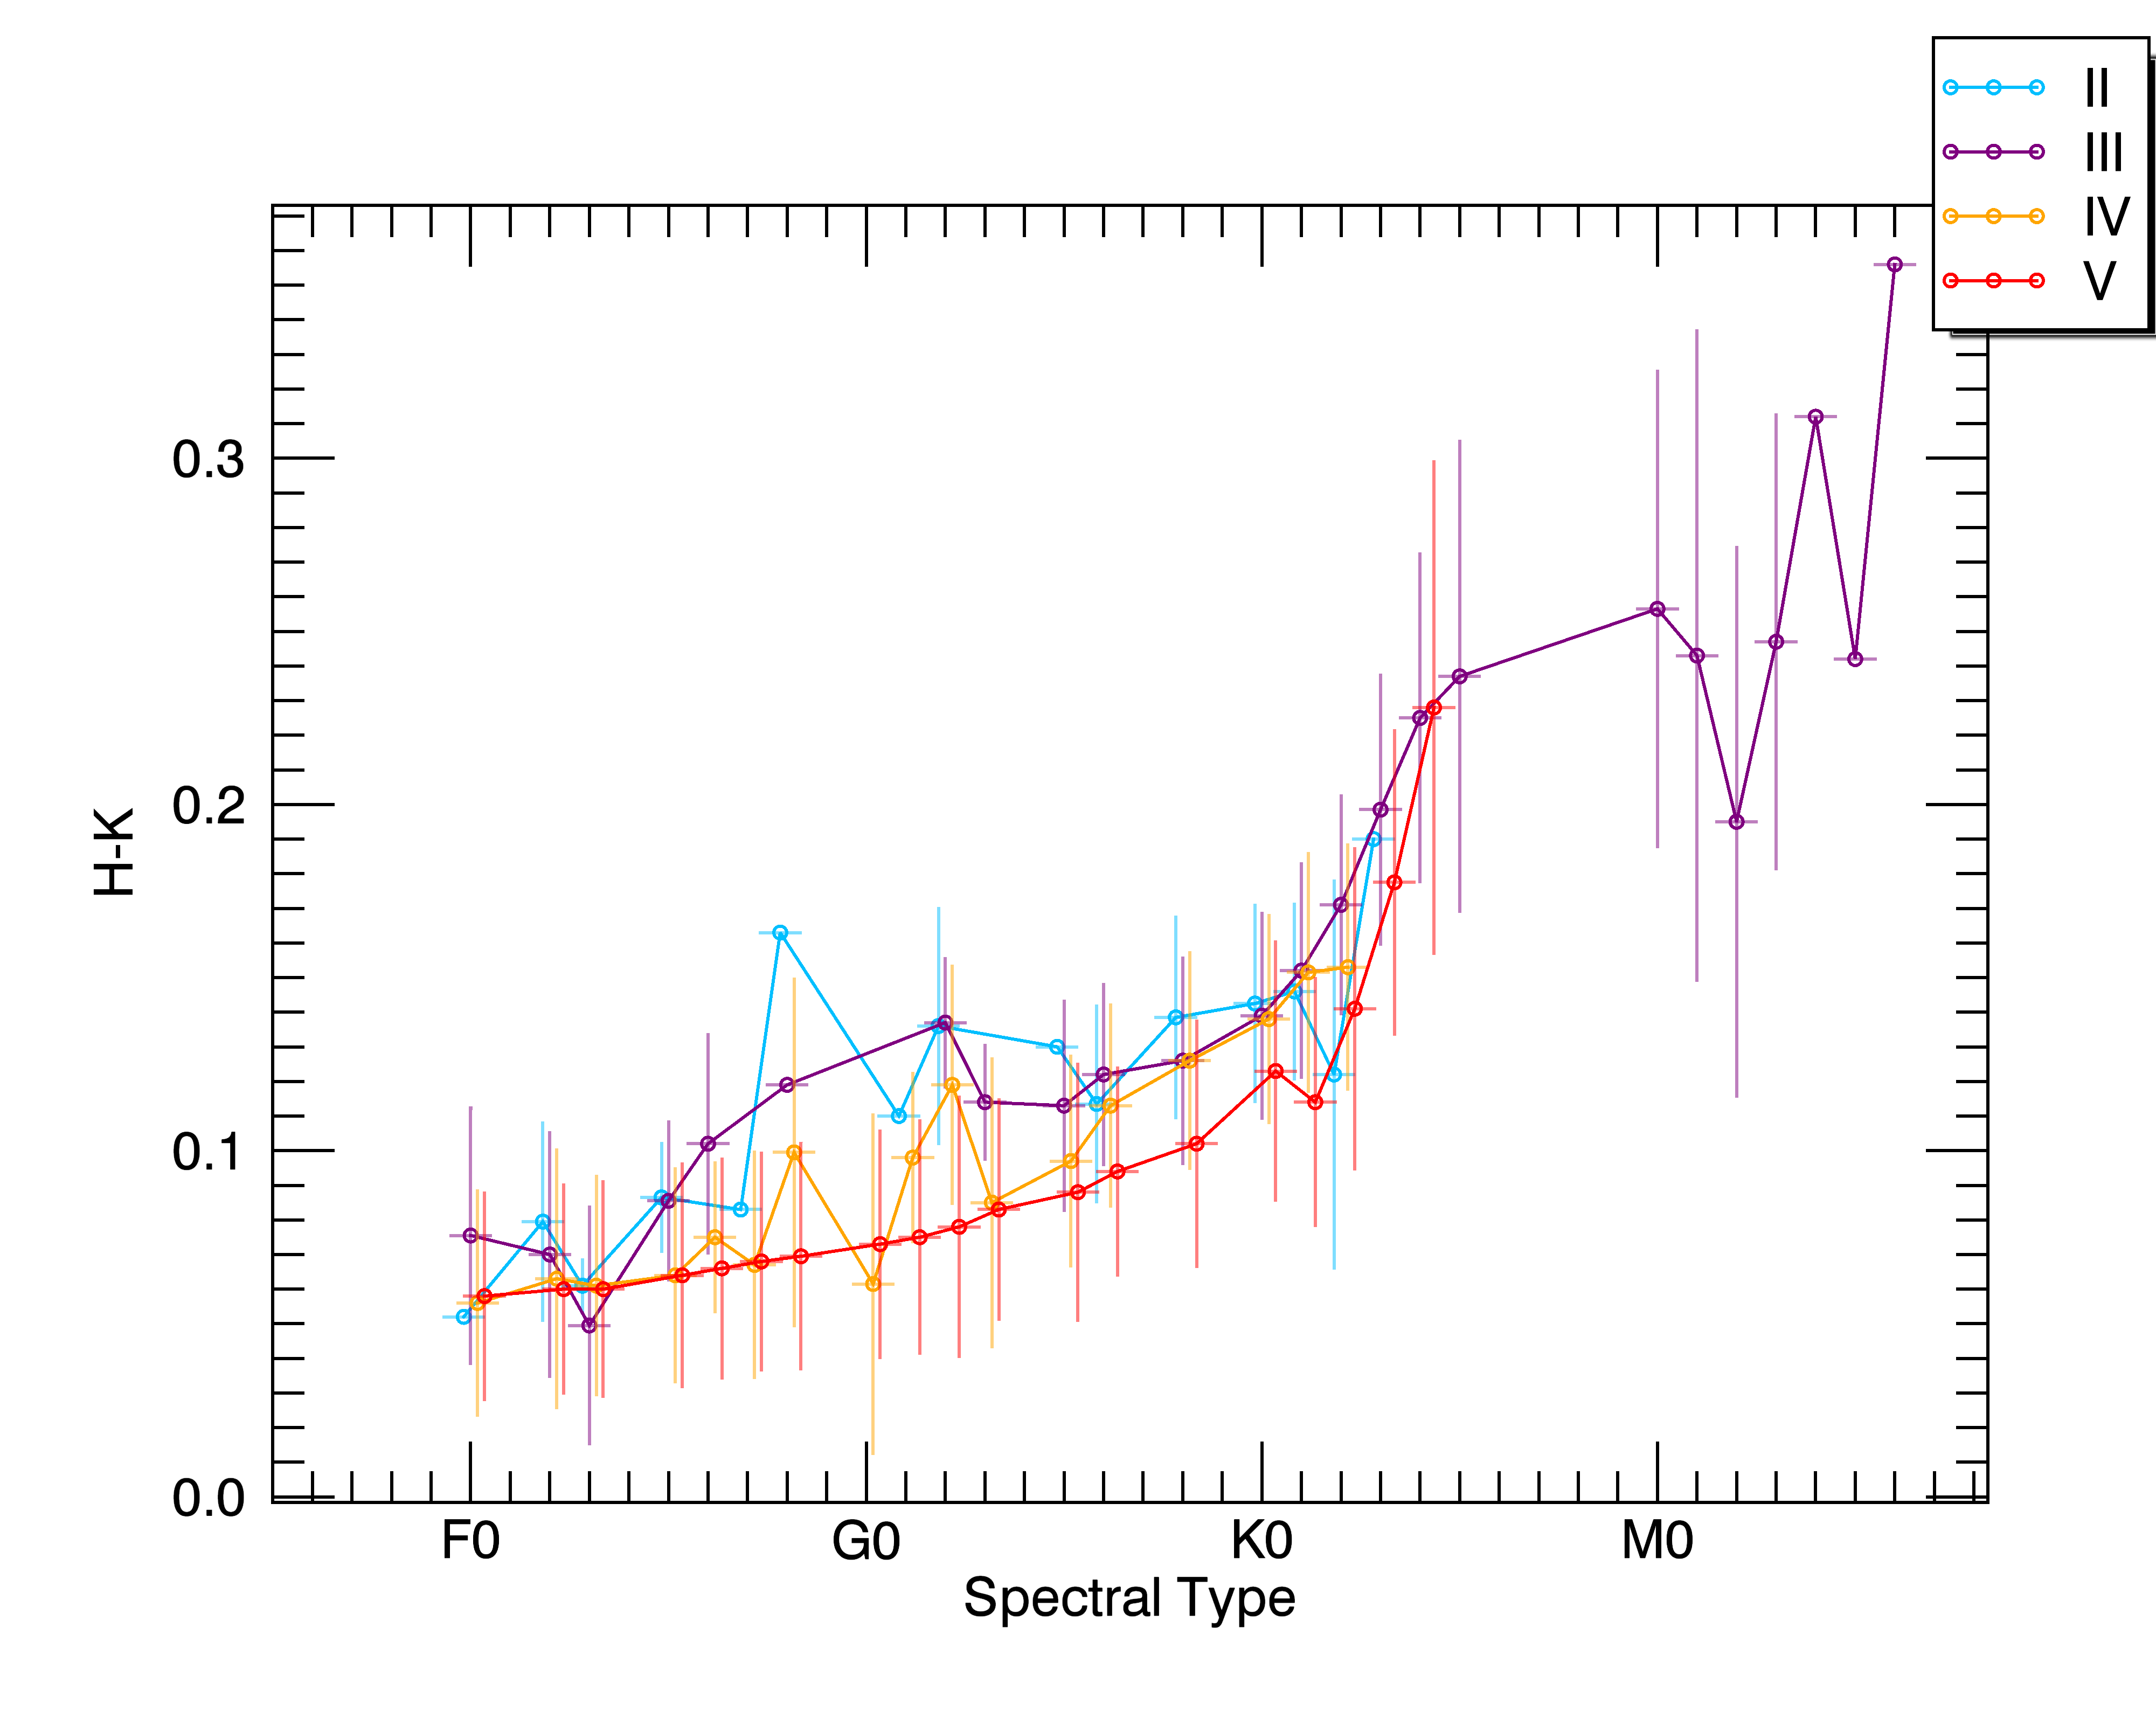
\includegraphics[width=0.8\textwidth,clip=true]{Figures/subtype_bar/SPT_H-K.png}
\end{minipage}\qquad
\begin{minipage}[b]{\textwidth}
    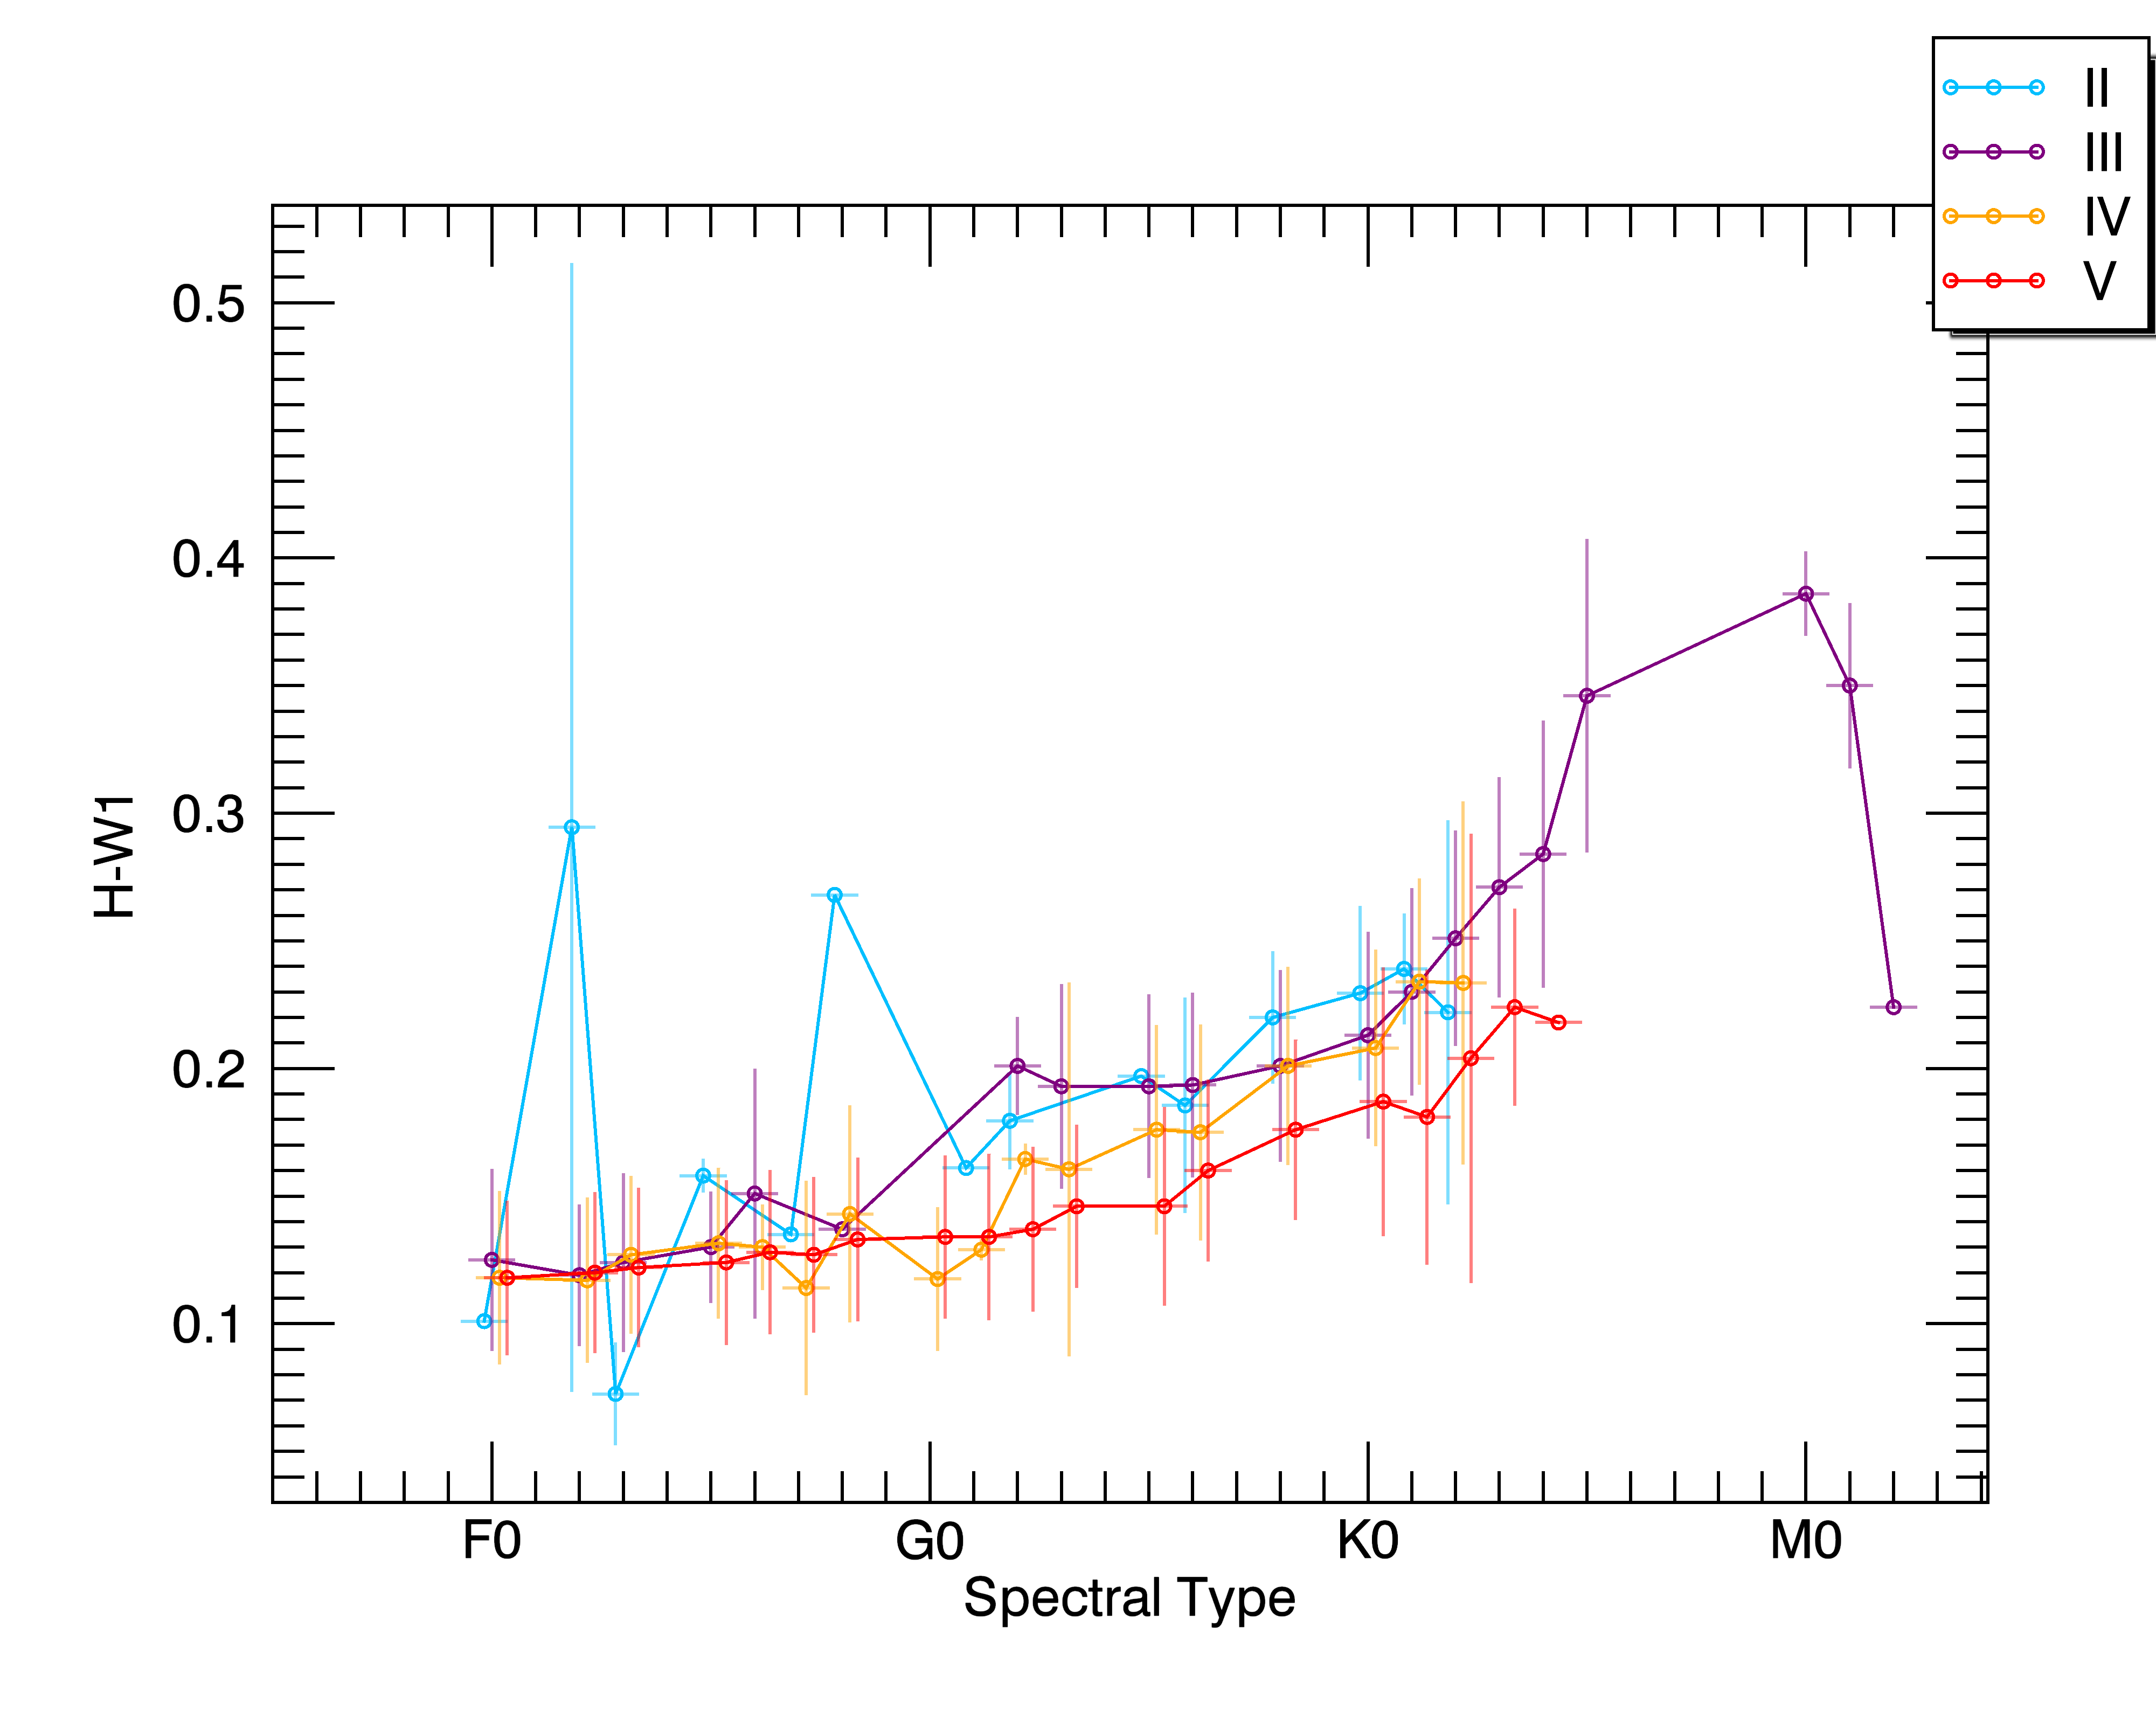
\includegraphics[width=0.8\textwidth,clip=true]{Figures/subtype_bar/SPT_H-W1.png}
\end{minipage}
\end{figure*}
\chapter{Color probability distributions}\label{Appendix:3}
We present average colors $J-W_{1}$ and $J-W_{2}$, for which we found a significant difference among dwarf and giant stars of the same spectral type (G0--K3). 
\begin{table}[t]
\scriptsize
\centering
\caption{Average \jwone and \jwone colors and separations}
\label{table:color_avgs}
\begin{center}
    \addtolength{\leftskip} {-2cm}
    \addtolength{\rightskip}{-2cm}
    \begin{tabular}{c|rrr|rrr}
    \toprule
    Spectral & & \jwone & & & \jwtwo & \\
    Type & Dwarfs & Giants & $\Delta$(mag.) & Dwarfs & Giants &  $\Delta$(mag.) \\ \midrule
    B2 & \minus0.025 & \minus0.123 & \minus0.098 & 0.083 & \minus0.054 & \minus0.137 \\
    B3 & \minus0.100 & \minus0.023 & 0.077 & \minus0.115 & \minus0.041 & 0.075 \\
    B4 & \minus0.086 & \minus0.046 & 0.040 & \minus0.150 & 0.009 & 0.159 \\
    B5 & 0.005 & \minus0.024 & \minus0.028 & 0.035 & \minus0.024 & \minus0.059 \\
    B6 & \minus0.016 & \minus0.019 & \minus0.003 & \minus0.033 & \minus0.055 & \minus0.022 \\
    B7 & \minus0.079 & \minus0.046 & 0.033 & \minus0.072 & \minus0.038 & 0.035 \\
    B8 & \minus0.008 & \minus0.058 & \minus0.050 & \minus0.008 & \minus0.076 & \minus0.067 \\
    B9 & 0.044 & 0.016 & \minus0.028 & 0.018 & \minus0.004 & \minus0.022 \\
    A0 & 0.078 & 0.146 & 0.068 & 0.052 & 0.141 & 0.088 \\
    A1 & 0.107 & 0.143 & 0.036 & 0.082 & 0.123 & 0.041 \\
    A2 & 0.126 & 0.162 & 0.036 & 0.098 & 0.135 & 0.037 \\
    A3 & 0.139 & 0.166 & 0.028 & 0.113 & 0.141 & 0.028 \\
    A4 & 0.169 & 0.181 & 0.012 & 0.142 & 0.160 & 0.018 \\
    A5 & 0.164 & 0.190 & 0.026 & 0.141 & 0.161 & 0.020 \\
    A6 & 0.176 & 0.205 & 0.029 & 0.153 & 0.178 & 0.025 \\
    A7 & 0.192 & 0.207 & 0.016 & 0.163 & 0.180 & 0.017 \\
    A8 & 0.224 & 0.214 & \minus0.009 & 0.204 & 0.191 & \minus0.013 \\
    A9 & 0.239 & 0.226 & \minus0.013 & 0.214 & 0.204 & \minus0.009 \\
    F0 & 0.268 & 0.253 & \minus0.015 & 0.244 & 0.237 & \minus0.008 \\
    F2 & 0.292 & 0.274 & \minus0.019 & 0.267 & 0.258 & \minus0.010 \\
    F3 & 0.312 & 0.305 & \minus0.008 & 0.284 & 0.289 & 0.005 \\
    F5 & 0.338 & 0.336 & \minus0.002 & 0.305 & 0.308 & 0.003 \\
    F6 & 0.354 & 0.338 & \minus0.016 & 0.317 & 0.311 & \minus0.006 \\
    F7 & 0.372 & 0.372 & 0.000 & 0.334 & 0.333 & \minus0.001 \\
    F8 & 0.373 & 0.476 & 0.103 & 0.332 & 0.493 & 0.161 \\
    G0 & 0.390 & 0.432 & 0.042 & 0.346 & 0.387 & 0.041 \\
    G1 & 0.401 & 0.498 & 0.097 & 0.357 & 0.530 & 0.172 \\
    G2 & 0.420 & 0.536 & 0.116 & 0.377 & 0.570 & 0.192 \\
    G3 & 0.445 & 0.562 & 0.117 & 0.396 & 0.516 & 0.120 \\
    G5 & 0.490 & 0.628 & 0.138 & 0.448 & 0.608 & 0.160 \\
    G6 & 0.518 & 0.641 & 0.123 & 0.463 & 0.594 & 0.131 \\
    G8 & 0.611 & 0.694 & 0.083 & 0.547 & 0.655 & 0.108 \\
    K0 & 0.706 & 0.735 & 0.029 & 0.637 & 0.732 & 0.095 \\
    K1 & 0.697 & 0.800 & 0.102 & 0.637 & 0.774 & 0.137 \\
    K2 & 0.721 & 0.877 & 0.156 & 0.709 & 0.895 & 0.187 \\
    K3 & 0.871 & 0.983 & 0.111 & 0.879 & 1.102 & 0.224 \\

    \bottomrule
    \addlinespace[10pt]
    \end{tabular}

\caption{This figure displays the average color (in units of magnitude) for both \jwone and \jwtwo of two luminosity groups and spectral subtype bins as described in Chapter \ref{subsec:tdist_stats}. The averages were calculated from fitting color to a Student's t-distribution function. Luminosity and spectral class information was retrieved from the Michigan Spectral Atlases, and photometry was taken from cross-matching to 2MASS/WISE catalogs (Chapter \ref{chap:2}). The star count for each bin from which the averages have been calculated are stated in Table \ref{table:bin_counts}. All sub-types listed have a least 4 stars or more, which is the minimum requirement to calculate a reliable average from fitting to a Student's t-distribution (Chapter \ref{subsec:tdist_stats}). The third column ($\Delta$) represents the difference of the average giant color from the average dwarf color for each individual bin and for a single color. We note that the greatest differences, or separations between dwarfs and giants, occurs approximately for spectral types G0--K3, where we have an average separation of $\sim$0.10 and $\sim$0.14 mag for \jwone and \jwtwo respectively. As expected, the color difference is positive, so giants are redder than dwarfs for each of these sub-type bins. The degree of color separation for all bins is mapped visually in Figures \ref{fig:periodic-delta-jw1} and \ref{fig:periodic-delta-jw2}.}.
\end{center}
\end{table}
\chapter{Sample applications with color probabilities }\label{Appendix:4}

We present two potential applications of using the dwarf-giant difference in colors \jwone and \jwtwo, reduced proper motions in J-band (\ref{sec:RPM}) and combining color probabilities with a galactic model (\ref{sec:galactic_model}) .

\section{Reduced proper motions} \label{sec:RPM}

All of the Michigan stars are HD stars with GAIA parallaxes and proper motions. We cross-correlate the Michigan catalog with the GAIA First Data Release \citep[]{gaia1,gaia2,Lindegren2016}.  In Figure 8, we plot the standard reduced proper motion (${rpm}_J$) for the Michigan stars as a function of \jwtwo for spectral types from G0--K5 and luminosity class, using GAIA proper motions. In Figures \ref{fig:absolute_j_jw1} and D.2, we plot the absolute J-band magnitudes for the Michigan stars as function of \jwtwo for spectral types from G0--K5 and luminosity class, using GAIA parallaxes. From these plots, we see that the classification success rate of the Michigan catalog is high, but not perfect.

\section{Galactic population model} \label{sec:galactic_model}

We are considering also further finessing the color-luminosity class probability by relating color with position in the sky using a a synthetic galactic model of the Milky Way called TRILEGAL, but leave this for future work. Incorporating giant/dwarf population statistics, such as luminosity class number density as a function sky area, should help to further improve color as a tool to predict luminosity class, and for application to future surveys.

We plan to pick an ecliptic pole field as an application of calculating probabilistic luminosity class membership in a Bayesian framework. In particular, our priors are the mean and robust standard deviation of colors of each luminosity class as calculated in Chapter (\ref{subsec:median_stats}). We plan to use the TRILEGAL source counts to normalize these distributions with respect to one another, and integrate over a sample photometric measurement and its uncertainty.

% FIGURES =================

\begin{figure*}[t] 
  \begin{center}
      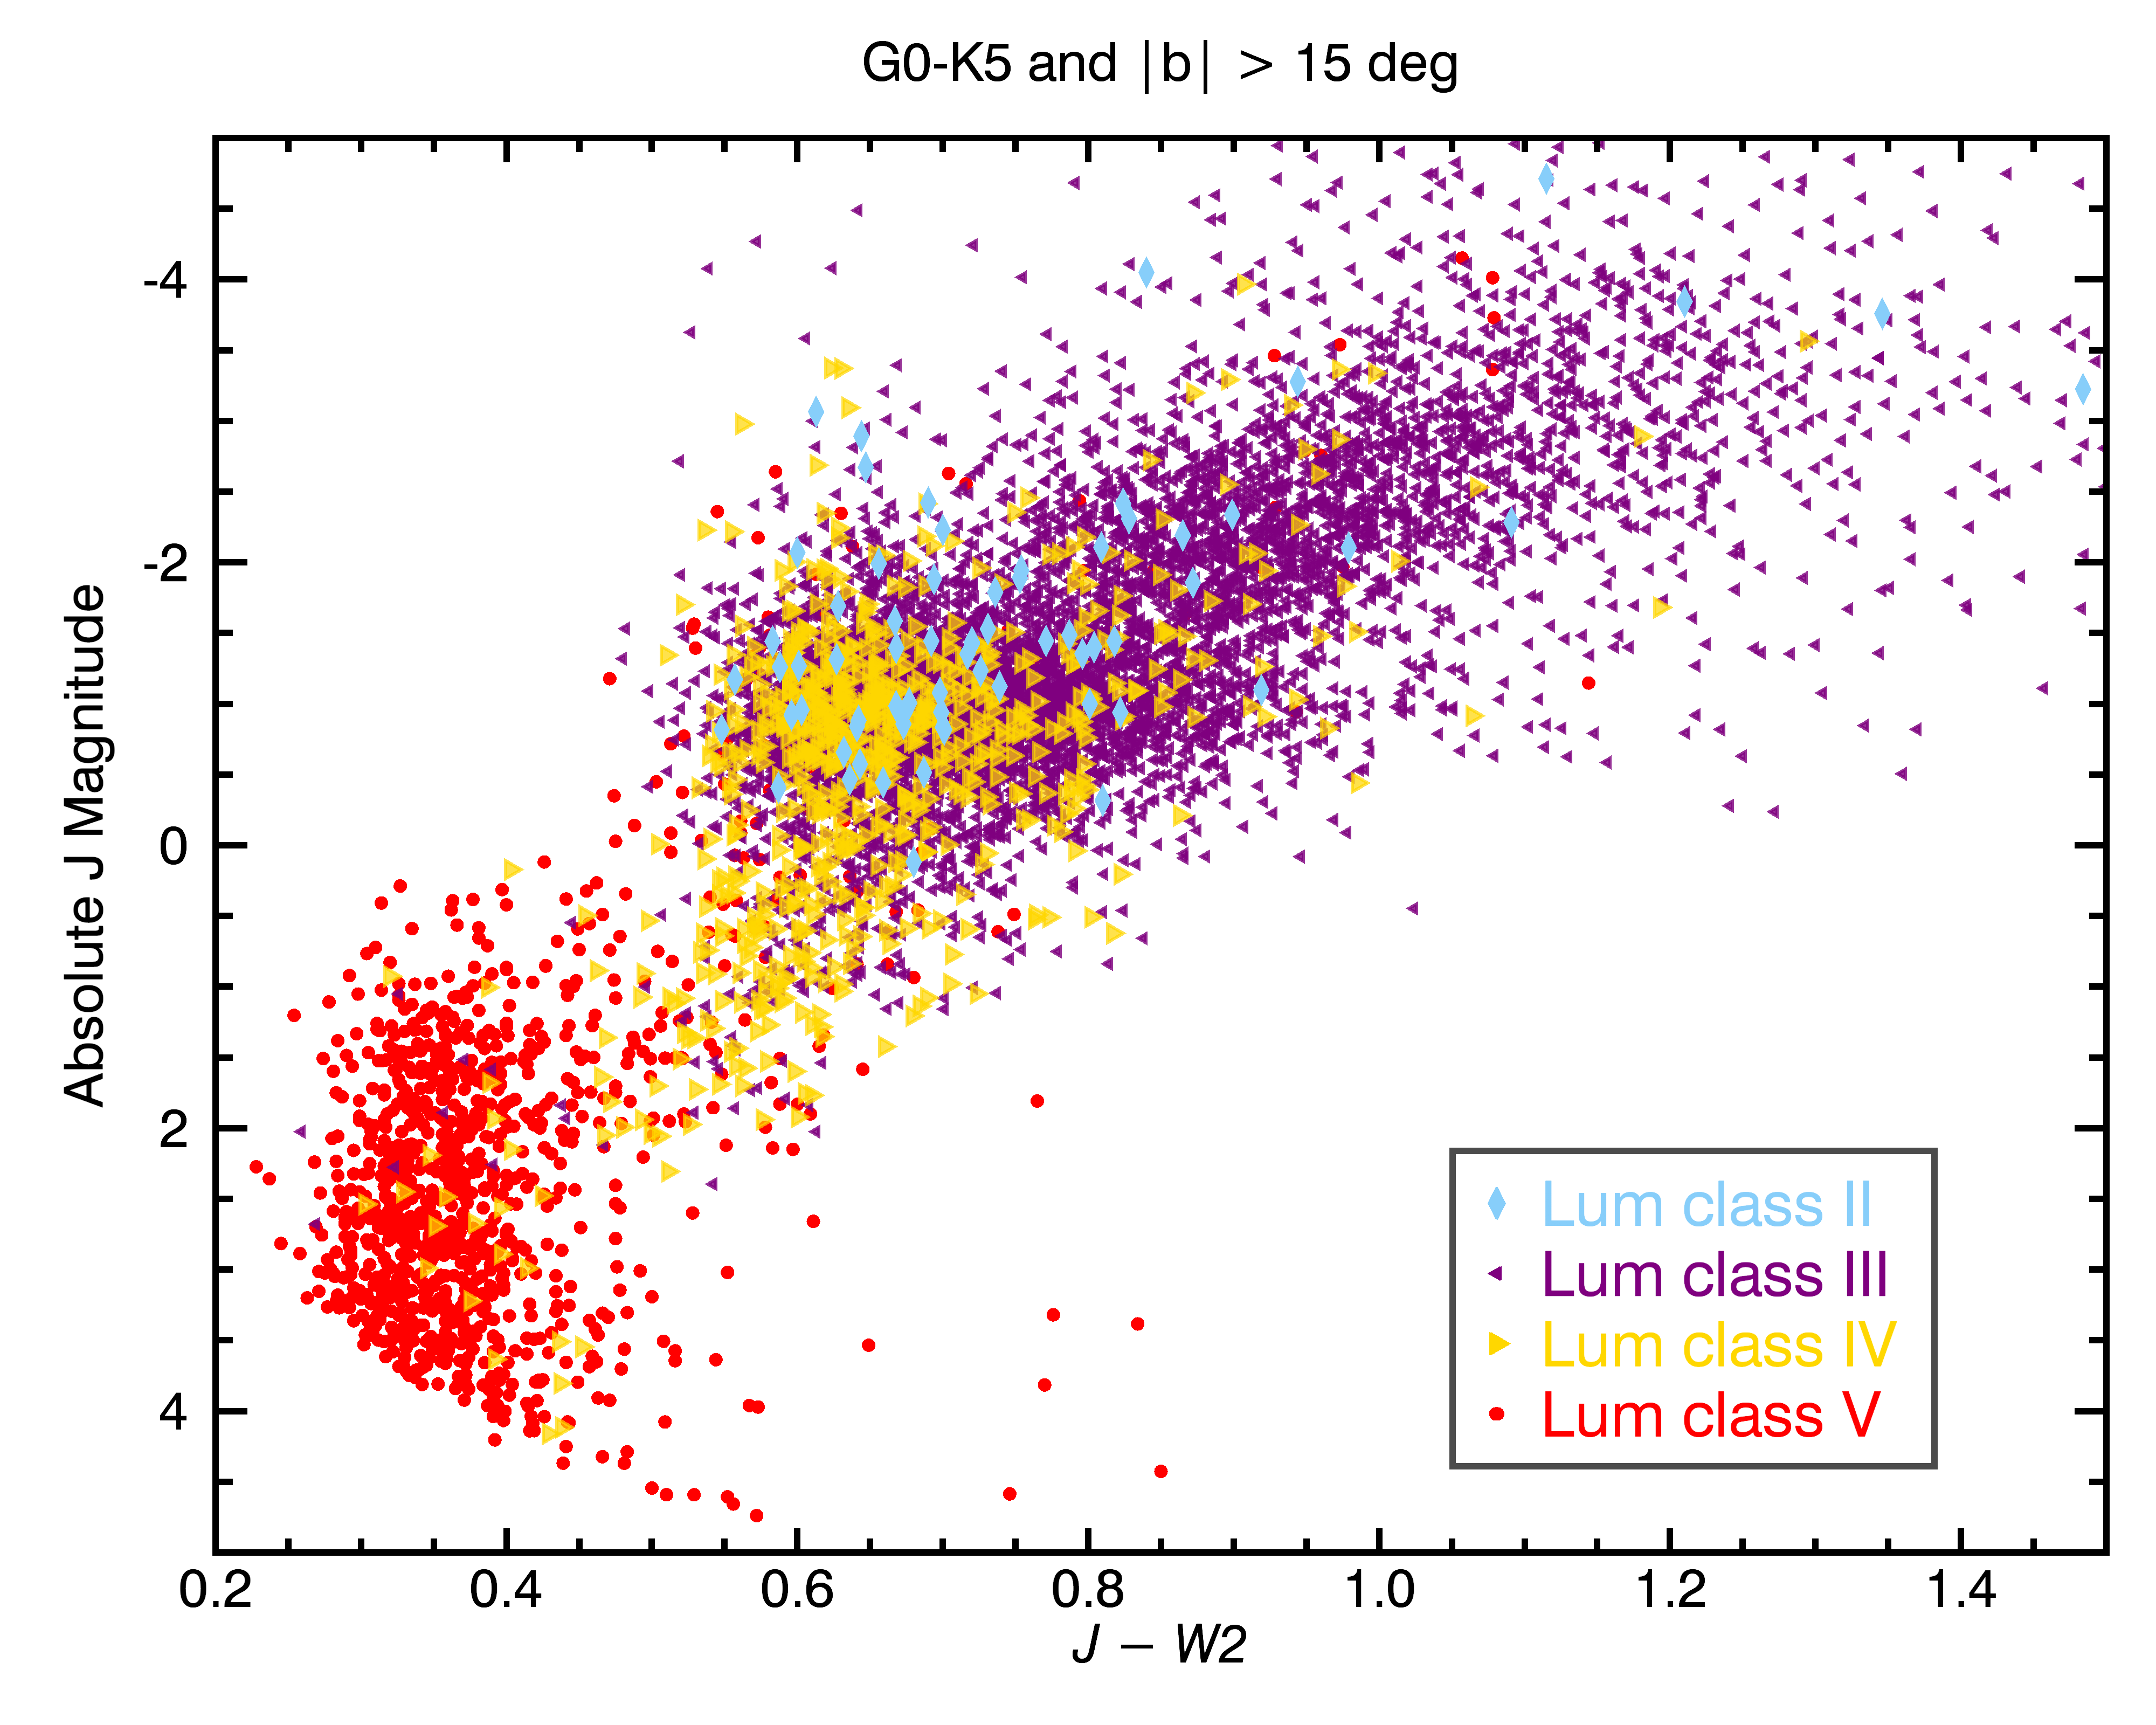
\includegraphics[width=1.0\textwidth,clip=true]{Figures/absolute_j/plot-J-W2-G0-K5-b15-abs-J.png}
 \end{center}
 \caption{Reduced $J$-band proper motion plot using \textit{GAIA} DR1 proper motions as a function of $J-W2$ color for Michigan Spectral Atlas stars with spectra types between G0 and K5 and galactic latitudes $|b|>15\deg$.  The different colors correspond to the different luminosity classes, and show a relatively clear separation between dwarfs and (sub-)giants.}\label{fig:absolute_j_jw1}
\end{figure*} 

\begin{figure*}[t] 
\begin{center}
    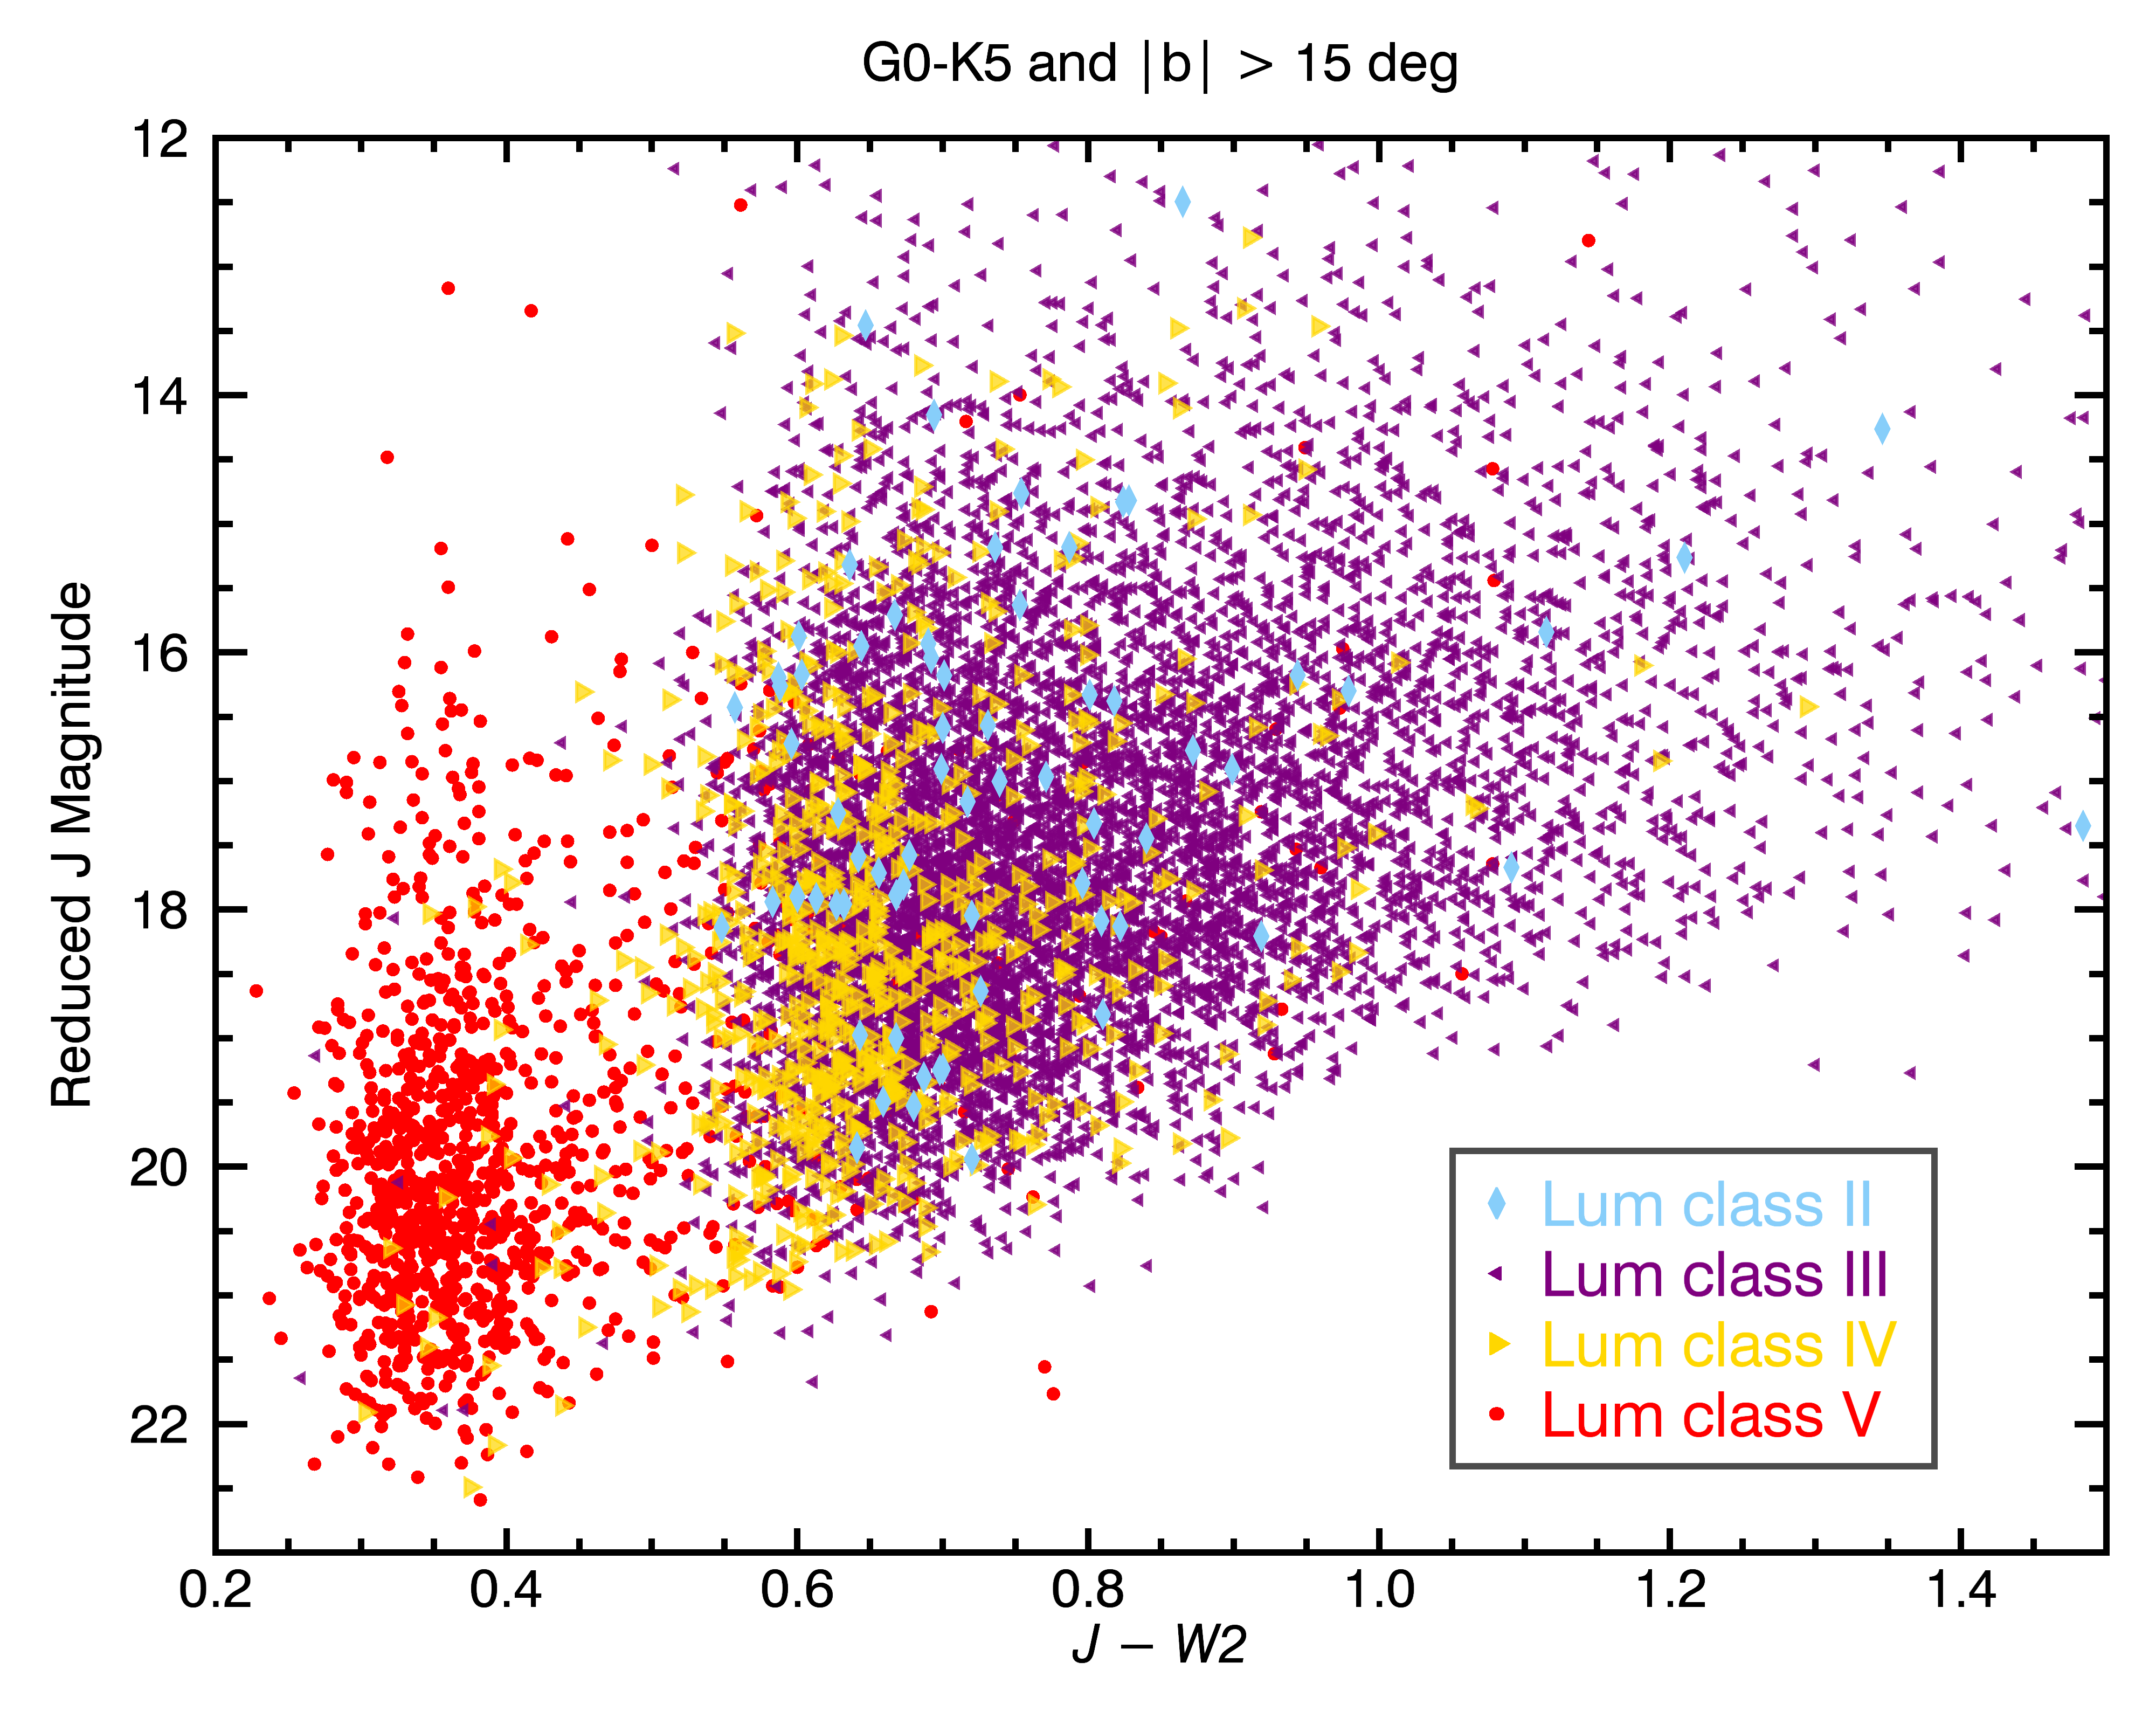
\includegraphics[width=1.0\textwidth,clip=true]{Figures/absolute_j/plot-J-W2-G0-K5-b15-rd-J.png}
\end{center}
\caption{The same as the previous figure, but for absolute $J$ band magnitudes using \textit{GAIA} DR1 parallaxes, validating the Michigan Spectral Atlas luminosity classes and the reduced proper motion approach.}\label{fig:reduced_j_jw2}
\end{figure*}
\end{appendices}

\backmatter

\bibliographystyle{aasjournal}
\bibliography{citations.bib}

\end{document}